
\documentclass[tcc,numbers]{configs/coppe}
% package below turns darkmode on
\usepackage{xcolor} \pagecolor[rgb]{0,0,0} \color[rgb]{1,1,1}
\usepackage{amsmath,amssymb}
\usepackage{silence}
\usepackage{hyperref}
\WarningFilter[pdftoc]{hyperref}{Token not allowed in a PDF string}

\makelosymbols
\makeloabbreviations

\begin{document}
  \title{Espectro de Modulação Aplicado ao Processamento de Fala}
  % \title{Aplicação do Espectro de Modulação no Processamento de Fala}
  \foreigntitle{Modulation Spectrum Applied over Speech Processing}
  \author{Miguel}{Fernandes de Sousa}
  \advisor{Prof.}{Luiz Wagner}{Pereira Biscainho}{D.Sc.}
  \advisor{Prof.}{Nome do Segundo Orientador}{Sobrenome}{Ph.D.}
  \advisor{Prof.}{Nome do Terceiro Orientador}{Sobrenome}{D.Sc.}

  \examiner{Prof.}{Nome do Primeiro Examinador Sobrenome}{D.Sc.}
  \examiner{Prof.}{Nome do Segundo Examinador Sobrenome}{Ph.D.}
  \examiner{Prof.}{Nome do Terceiro Examinador Sobrenome}{D.Sc.}
  \examiner{Prof.}{Nome do Quarto Examinador Sobrenome}{Ph.D.}
  \examiner{Prof.}{Nome do Quinto Examinador Sobrenome}{Ph.D.}
  \department{ELE}
  \date{07}{2022}

  \keyword{Espectrograma de Modulação}
  \keyword{Segunda palavra-chave}
  \keyword{Terceira palavra-chave}

  %TODO: remover \hbadness
  \hbadness=\maxdimen
  \maketitle

  % \hbadness=\maxdimen
  \frontmatter
  \dedication{Lorem Ipsum Est Es Un.}
  \hbadness=226

  \chapter*{Agradecimentos}

  Gostaria de agradecer a todos.

  \begin{abstract}

  Apresenta-se, nesta tese, \cite{timit} ...

  \end{abstract}

  \begin{foreignabstract}

  In this work, we present ...

  \end{foreignabstract}

  \tableofcontents
  \listoffigures
  \listoftables
  \printlosymbols
  \printloabbreviations

  \mainmatter
  %%________________________
  %% CHAPTER 01: Introdução
  \chapter{Introdução}
\section{Indaband}
A música, enquanto atividade e produto, permite o estabelecimento de laços sociais
entre musicistas e ouvintes.

A atividade musical permite que um conjunto de musicistas interaja e
comunique-se, facilitada quando os membros compartilham de uma mesma bagagem
cultural. Além disso, permite que a audiência estabeleça um vínculo com
o músico executor ou o conjunto de musicistas \cite{cook2021music}.

Por sua vez, a música enquanto produto permite o estabelecimento de laços sociais
entre os ouvintes, seja em uma sala de concerto no século XIX, em uma sala de estar
com um rádio ou um gramofone no século XX, ou em uma apresentação ao vivo na
plataforma Twitch no século XXI.

Durante a pandemia de COVID-19, estudantes de música precisaram adaptar seus
hábitos de prática musical para aulas remotas e práticas individuais. A prática
coletiva foi fortemente afetada, uma vez que as aulas e os ensaios presenciais
foram suspensos em uma série de instituições de ensino, dado o risco de
contaminação e a necessidade de distanciamento social \cite{nusseck2021musical}.

A prática remota síncrona, hoje, enfrenta uma série de desafios técnicos. A
latência entre os praticantes é o principal problema. O limiar da percepção
auditiva para atrasos é de cerca de 20 milissegundos, enquanto que sistemas VoIP
com latência de 150 milissegundos e \textit{jitter} de 30 milissegundos são
considerados de boa qualidade. A codificação associada à compressão do sinal e a
largura de banda também influenciam no atraso. Enquanto a latência em uma
comunicação instantânea não for inferior ao limiar da percepção, essa forma de
prática musical não será viável.

A principal alternativa é a prática musical colaborativa assíncrona. Nesse
cenário, cada praticante grava sua faixa de forma individual enquanto ouve as
demais faixas gravadas. Aplicações como \textit{BandLab}, \textit{Ableton Live}
e \textit{Soundtrap by Spotify} funcionam sob essa abordagem.

Uma segunda característica da prática musical coletiva, seja no contexto
presencial ou remoto, é a necessidade de encontrar outros interessados com
gostos musicais similares, instrumentos que se complementem, etc. Uma pessoa que
deseja tocar um estilo musical específico, incomum na região em que vive,
sofreria dessa dificuldade. Um meio de resolver esse problema é recorrer à
comunidades virtuais ou redes sociais. Ao encontrar outros interessados, caso a
distância impeça a prática presencial, a atividade pode ser realizada a partir
da prática musical colaborativa assíncrona. Plataformas como \textit{Cifra Club}
e \textit{Ultimate Guitar} permitem que usuários contribuam com tablaturas de
músicas e comentários, formando uma comunidade virtual.


Tanto a prática musical colaborativa assíncrona quanto a formação de comunidades
virtuais de música são problemas os quais o mercado oferece poucas soluções
integradas. Estações de trabalho de áudio digital (DAWs, do inglês
\textit{Digital Audio Workstations}) mais tradicionais, como \textit{Pro Tools},
\textit{Logic Pro} e \textit{Ableton Live} são desprovidos de funcionalidades de
interação social. \textit{Cifra Club} e \textit{Ultimate Guitar} não permitem a
gravação colaborativa de forma assíncrona. \textit{Soundtrap by Spotify} e
\textit{BandLab} permitem a edição colaborativa em tempo real, porém apenas o
último contém funcionalidades de interação e integração social entre usuários. A
aplicação \textit{Collab}, da Meta, preenchia parcialmente esses critérios antes
de ser descontinuada. O aplicativo móvel Indaband foi criado para ocupar esse
espaço pouco preenchido no mercado.

\begin{figure}[h]
    \centering
    \subfigure[]{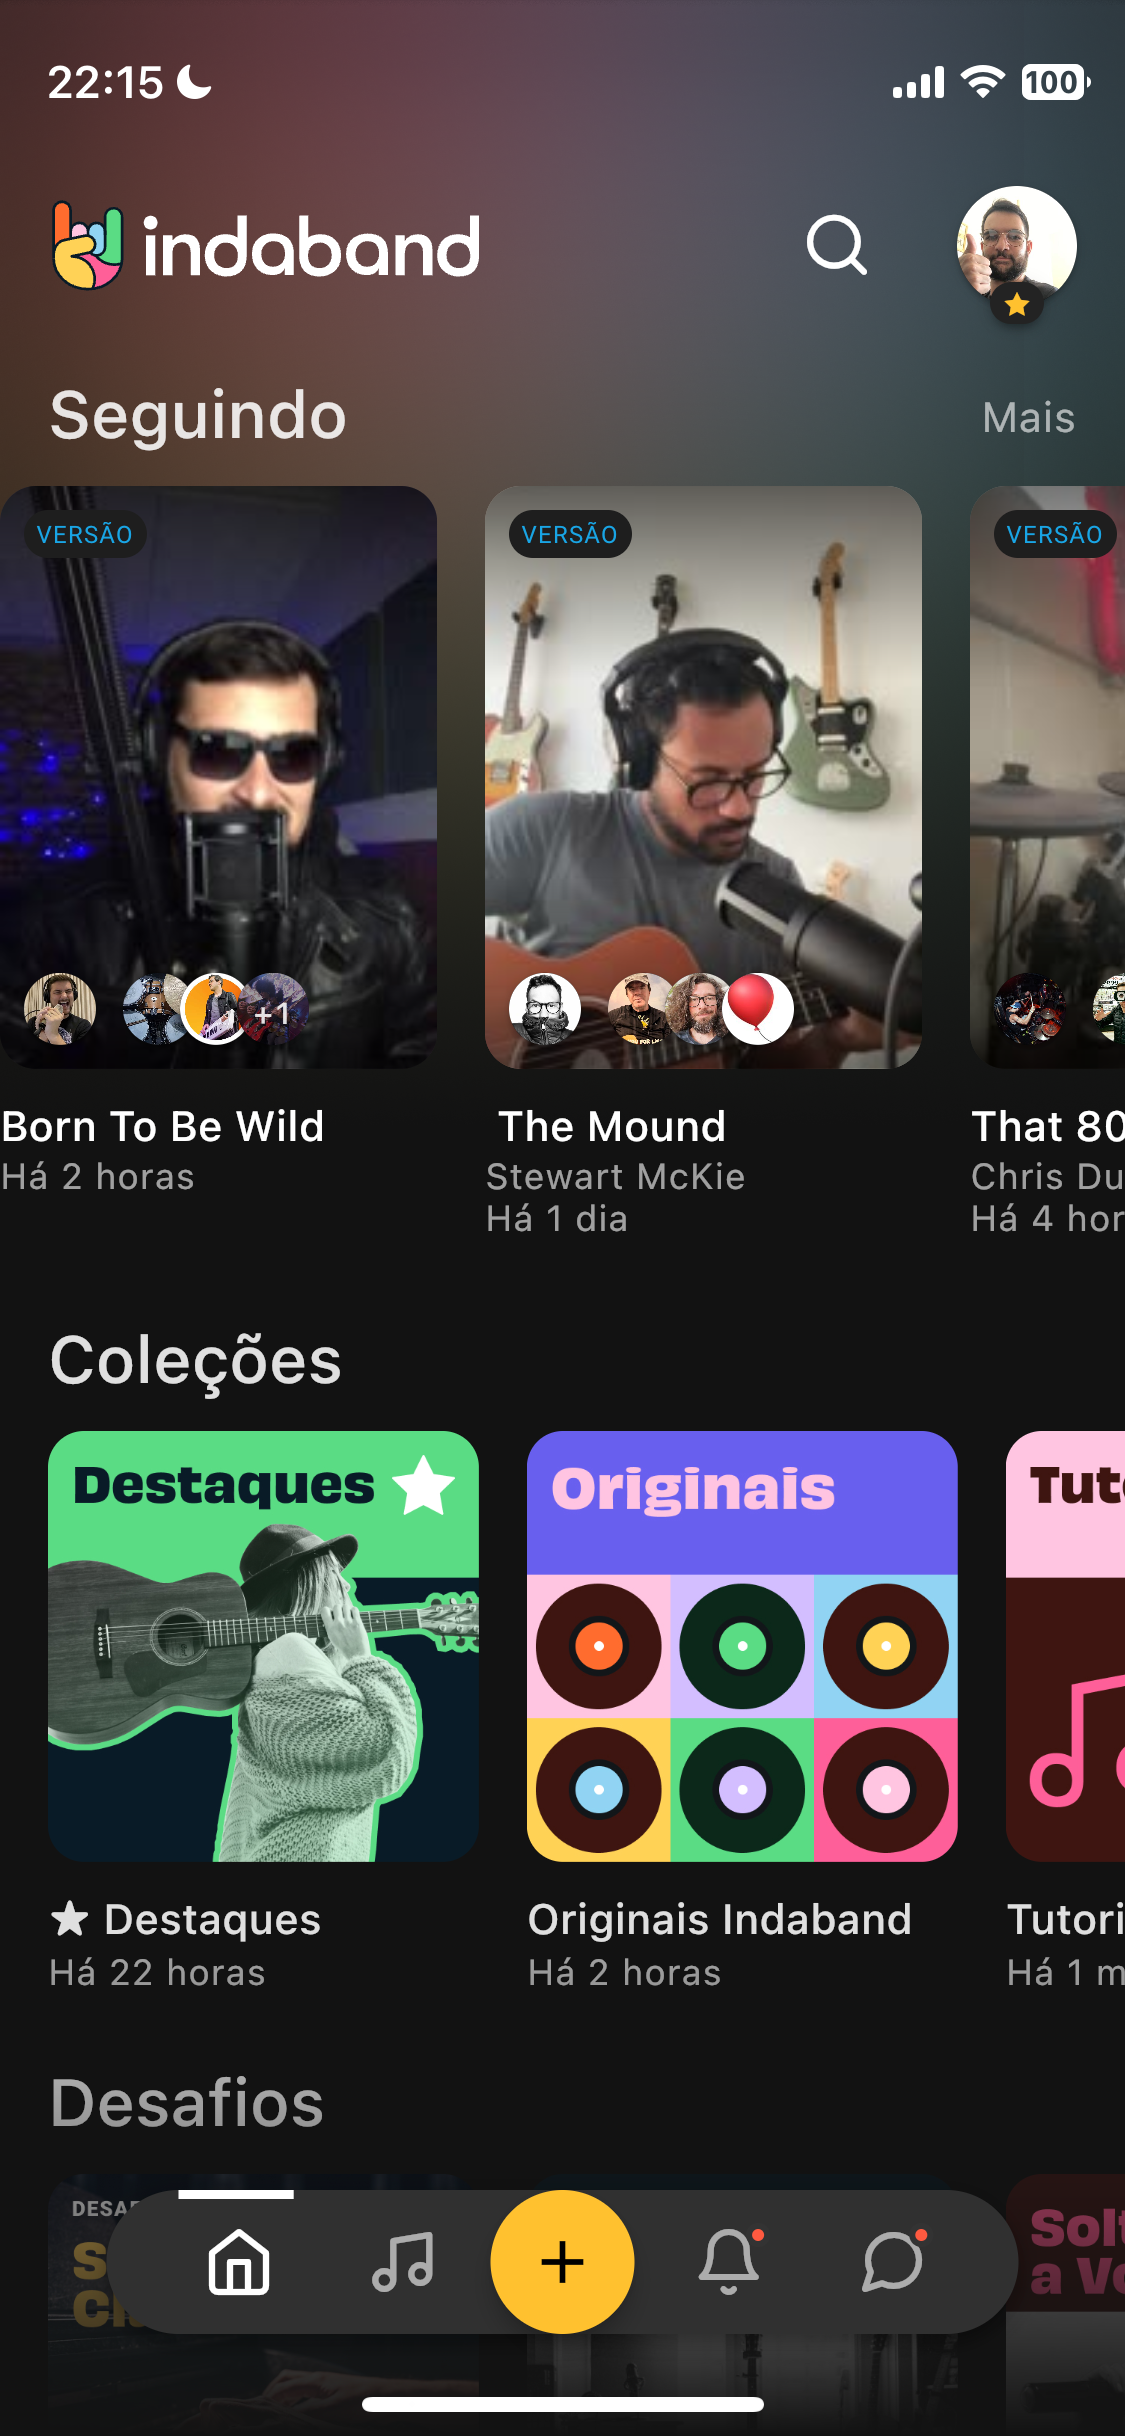
\includegraphics[width=0.24\textwidth]{chapters/chap01/images/inda/inda3.PNG}}
    \subfigure[]{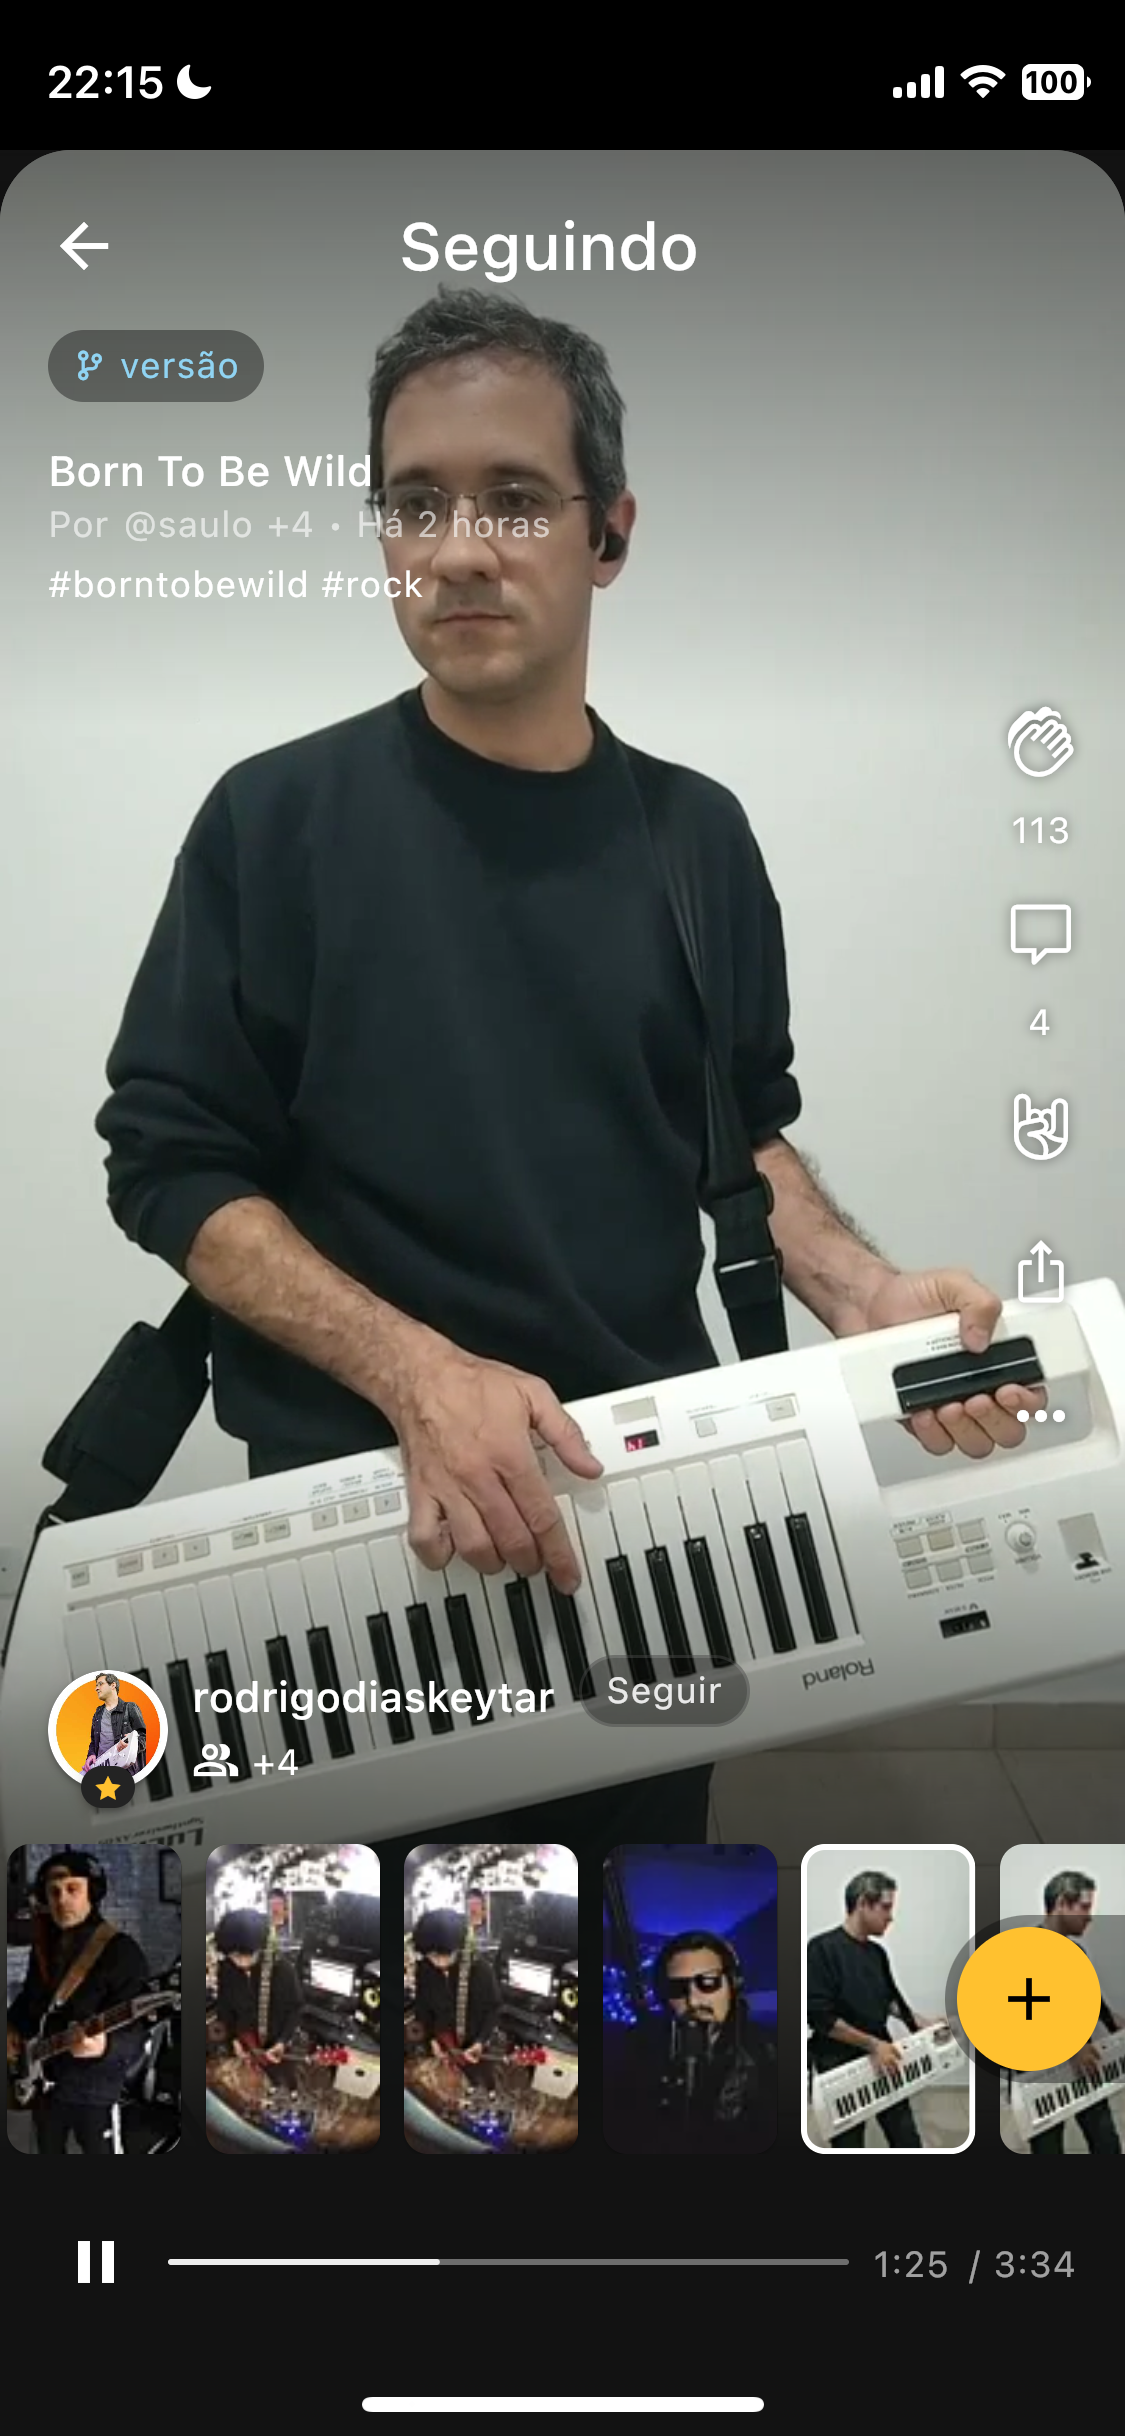
\includegraphics[width=0.24\textwidth]{chapters/chap01/images/inda/inda.PNG}}
    \subfigure[]{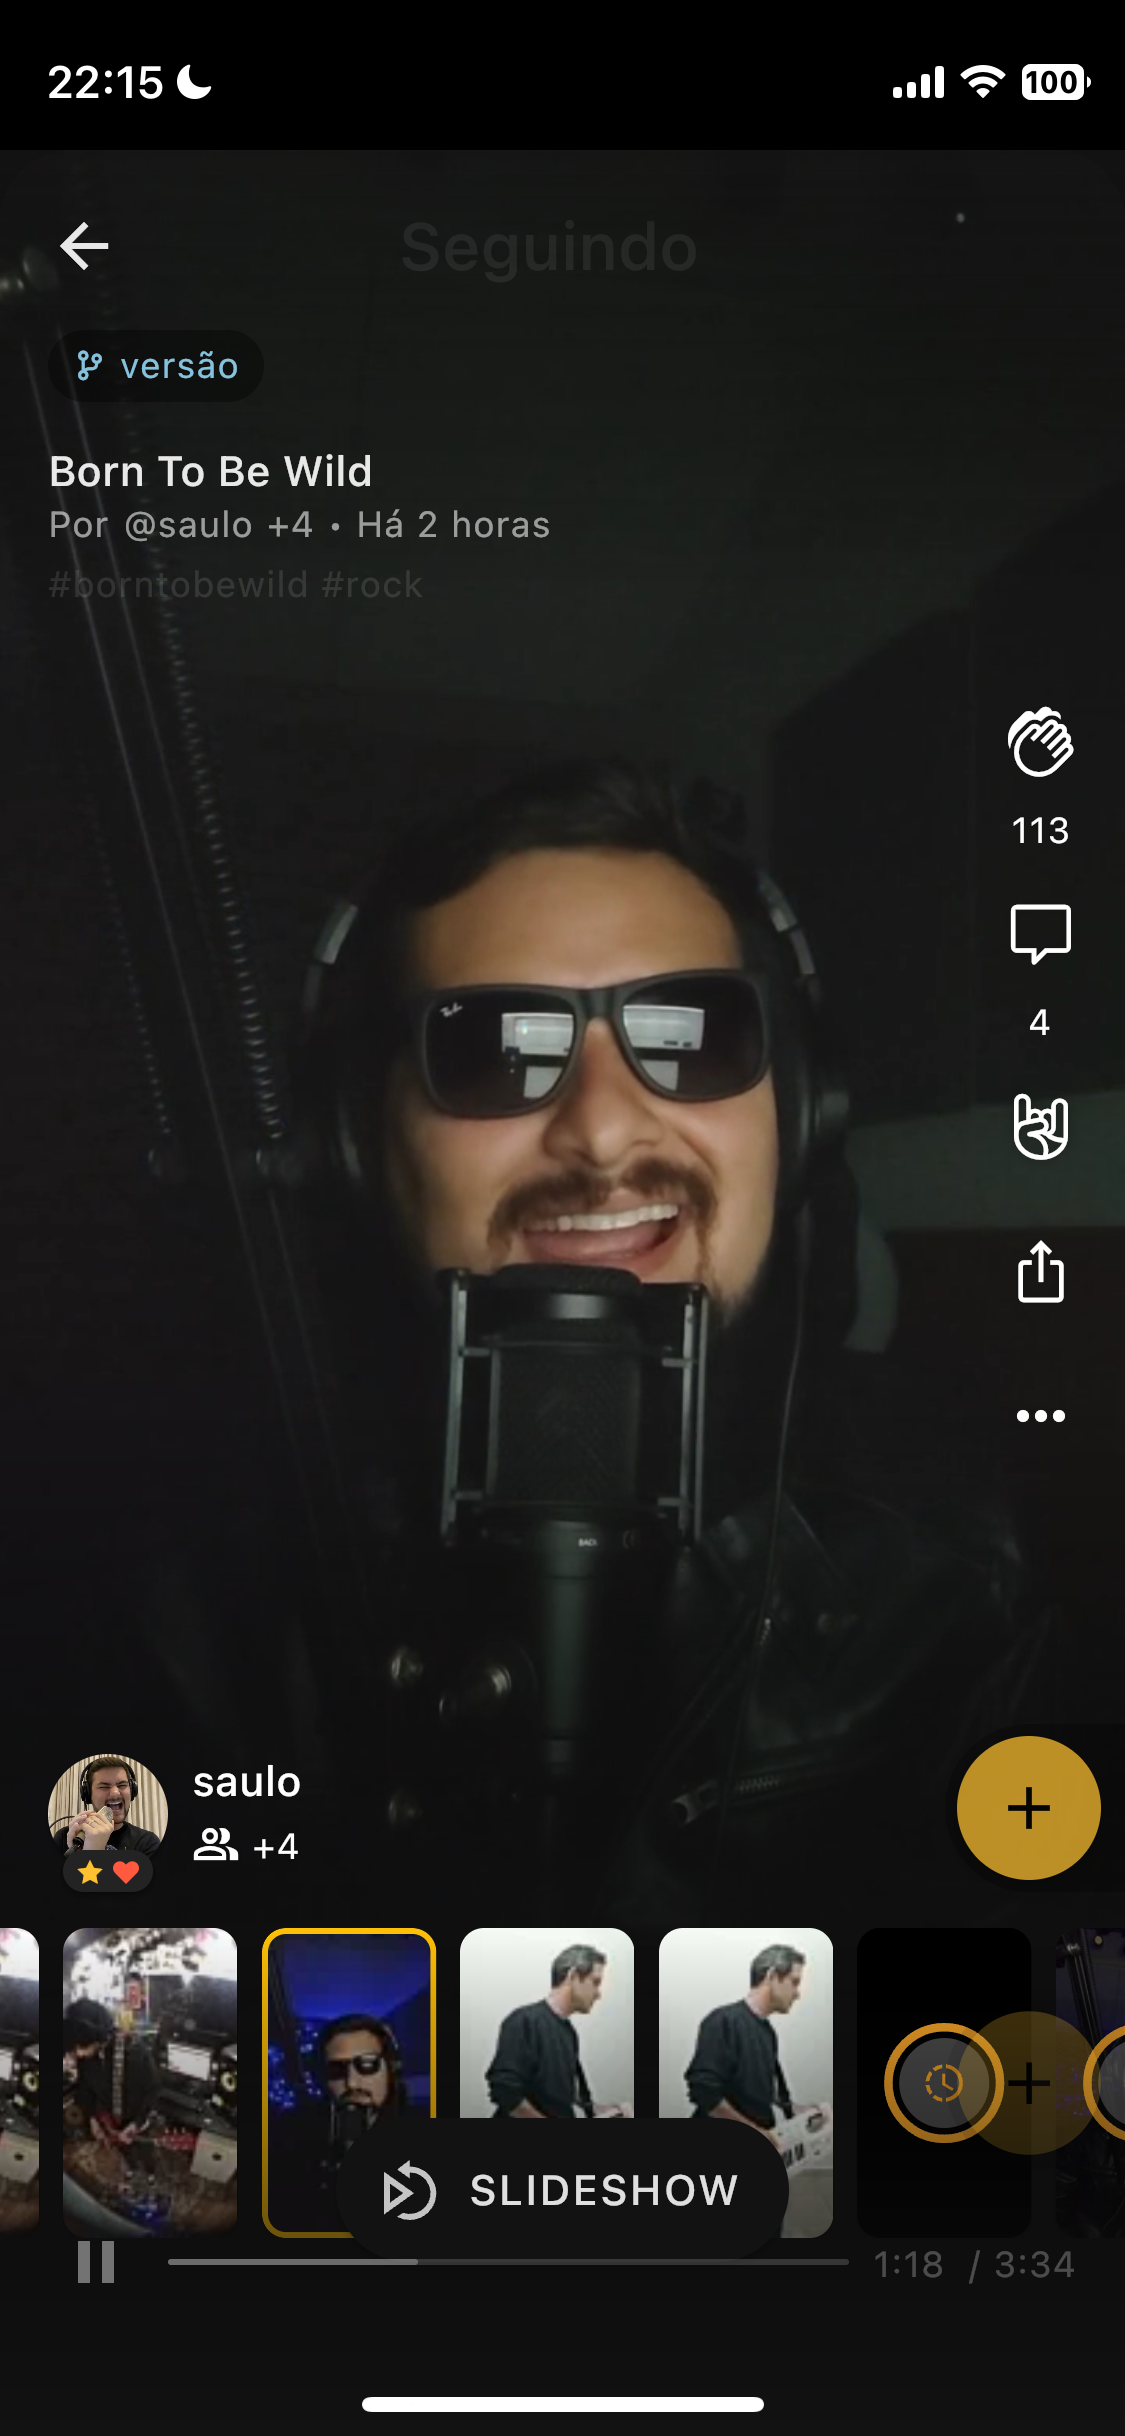
\includegraphics[width=0.24\textwidth]{chapters/chap01/images/inda/inda2.PNG}}
    \subfigure[]{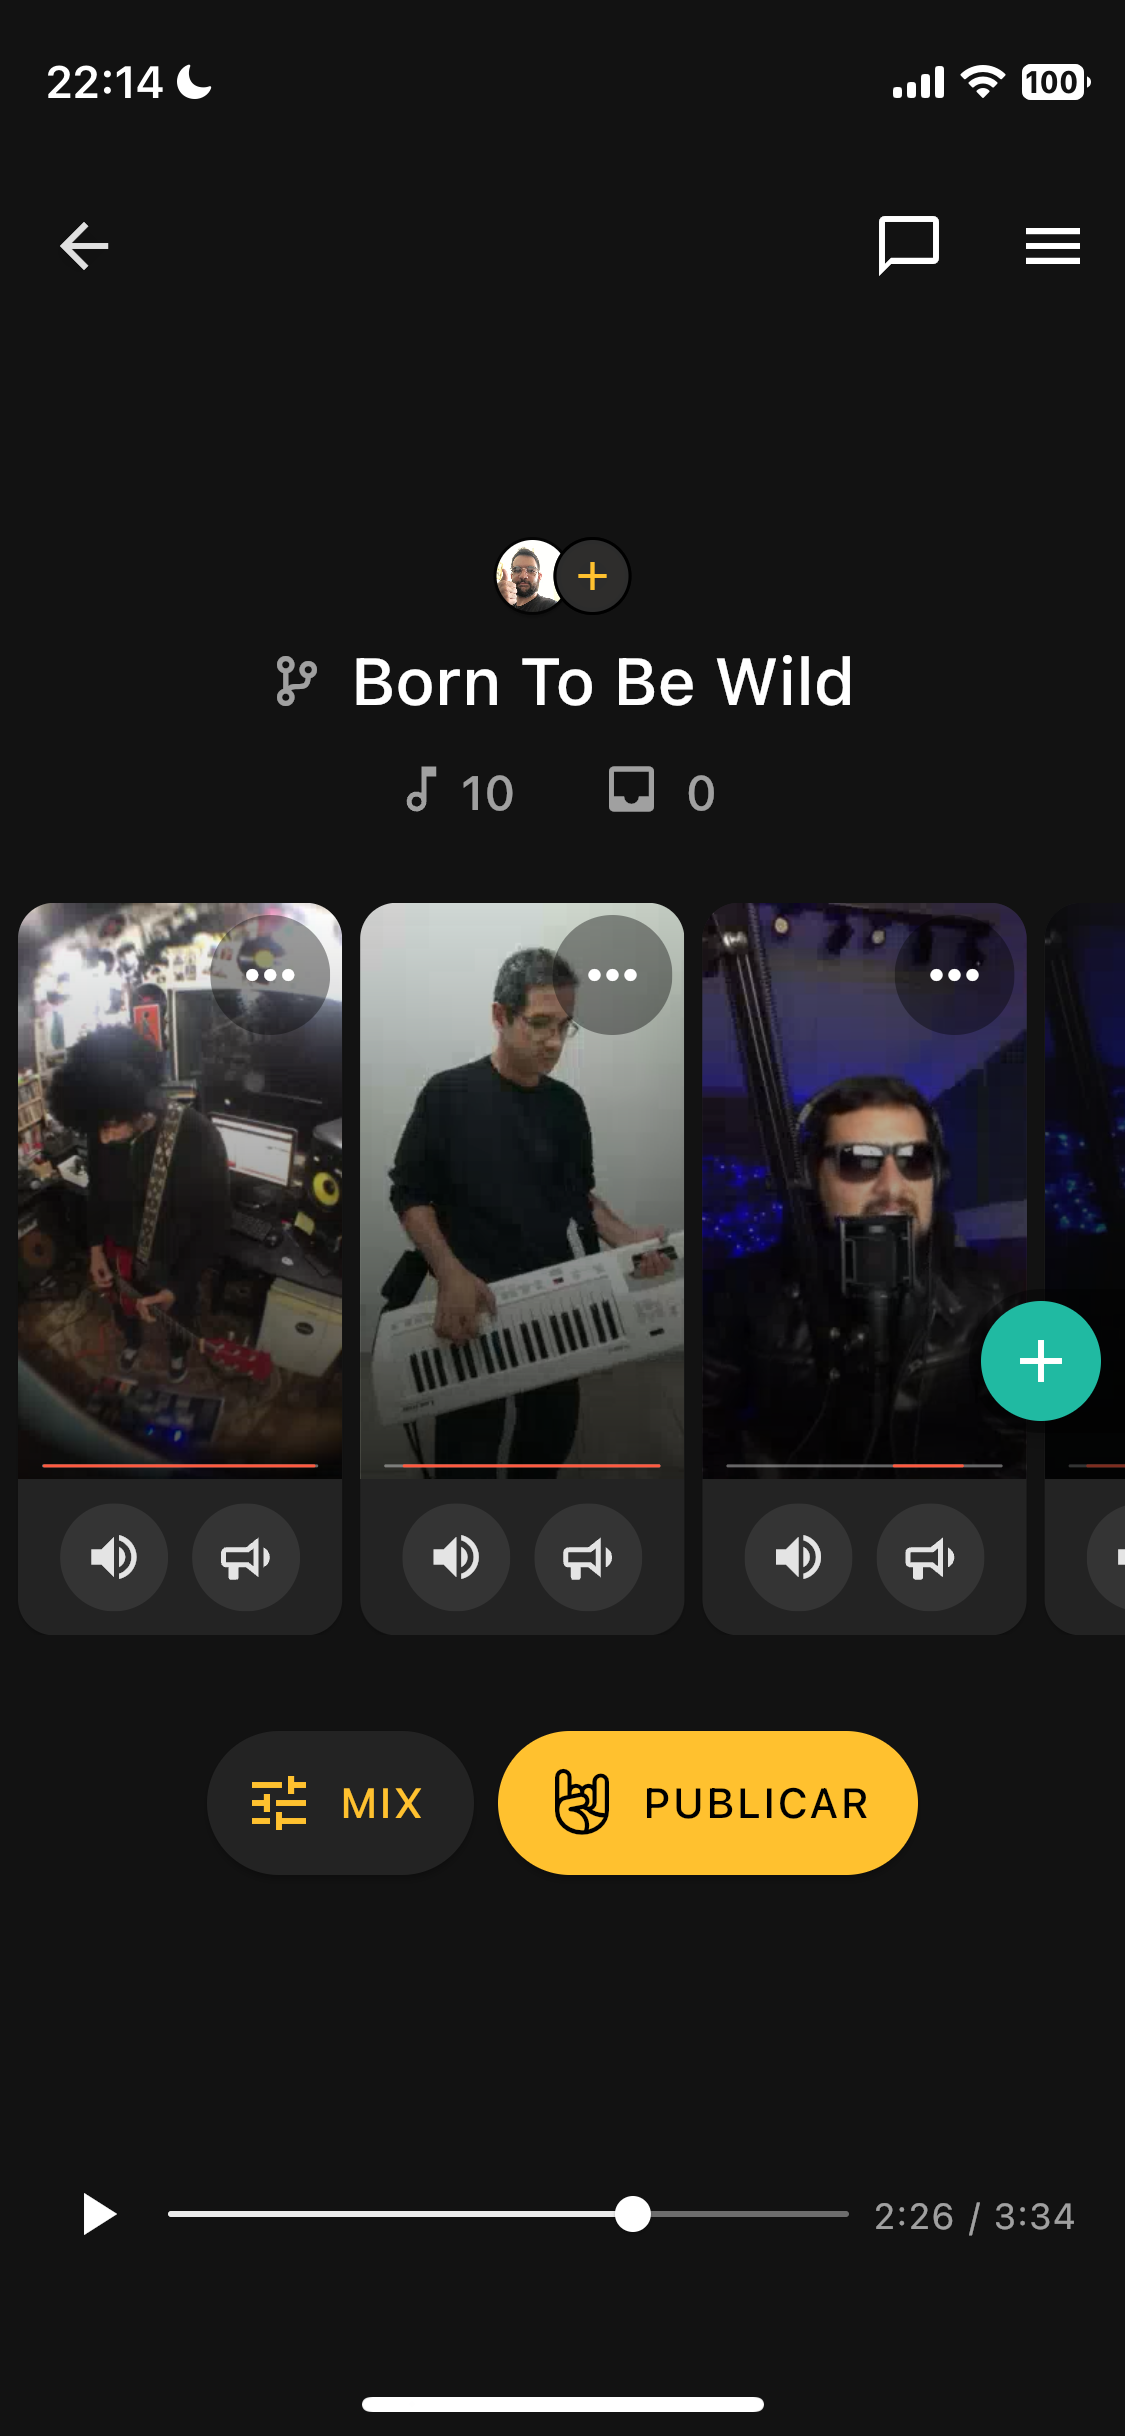
\includegraphics[width=0.24\textwidth]{chapters/chap01/images/inda/inda4.PNG}}
    \caption{Recursos do \textit{app Indaband}: (a) \textit{Home} (b) \textit{Feed} (c)
    \textit{Feed} (d) \textit{Studio}.}
    \label{fig:cap_tela}
\end{figure}

Indaband é uma aplicação móvel para distribuição e gravação de música
colaborativa e remota \cite{indaband}. A versão inicial foi disponibilizada
publicamente em Agosto de 2022. O quadro de funcionários é majoritariamente
brasileiro, enquanto que o produto possui distribuição global. A FIGURA
\ref{fig:cap_tela} exibe capturas de tela da interface visual.


O aplicativo móvel Indaband contém uma série de funcionalidades e abstrações
para a gravação e distribuição de música colaborativa. Para maior entendimento
do do sistema de recomendação a ser proposto, é necessário compreender as
principais entidades do aplicativo.


\subsubsection{Sessão}

Na aplicação, usuários podem criar sessões, que são ambientes colaborativos de
gravação entre os participantes. As sessões contam com ferramentas para gravação
e mixagem. O ambiente de pré-visualização, edição e produção da sessão chama-se
\textit{Studio}. Nesse ambiente, há funcionalidades de adição, edição,
remoção e mixagem de faixas. Sessão também é o nome dado ao conjunto de faixas
introduzidas pelos usuários que constituem uma determinada música.

A sessão contém uma funcionalidade de cabine de gravação, permitindo que os
participantes gravem faixas de áudio ou de vídeo. Além disso, o usuário pode
importar mídias de áudio ou de vídeo, tal que cada mídia importada equivale a
uma faixa.

O usuário que cria a sessão é considerado seu dono, enquanto os demais usuários
que aceitam o convite para ingressar são considerados participantes. Toda sessão
publicada é disponível para visualização pública e contém ao menos uma faixa. A
publicação pode ser posteriormente removida pelo dono da sessão.


\begin{figure}[h]
  \begin{center}
    \subfigure[]{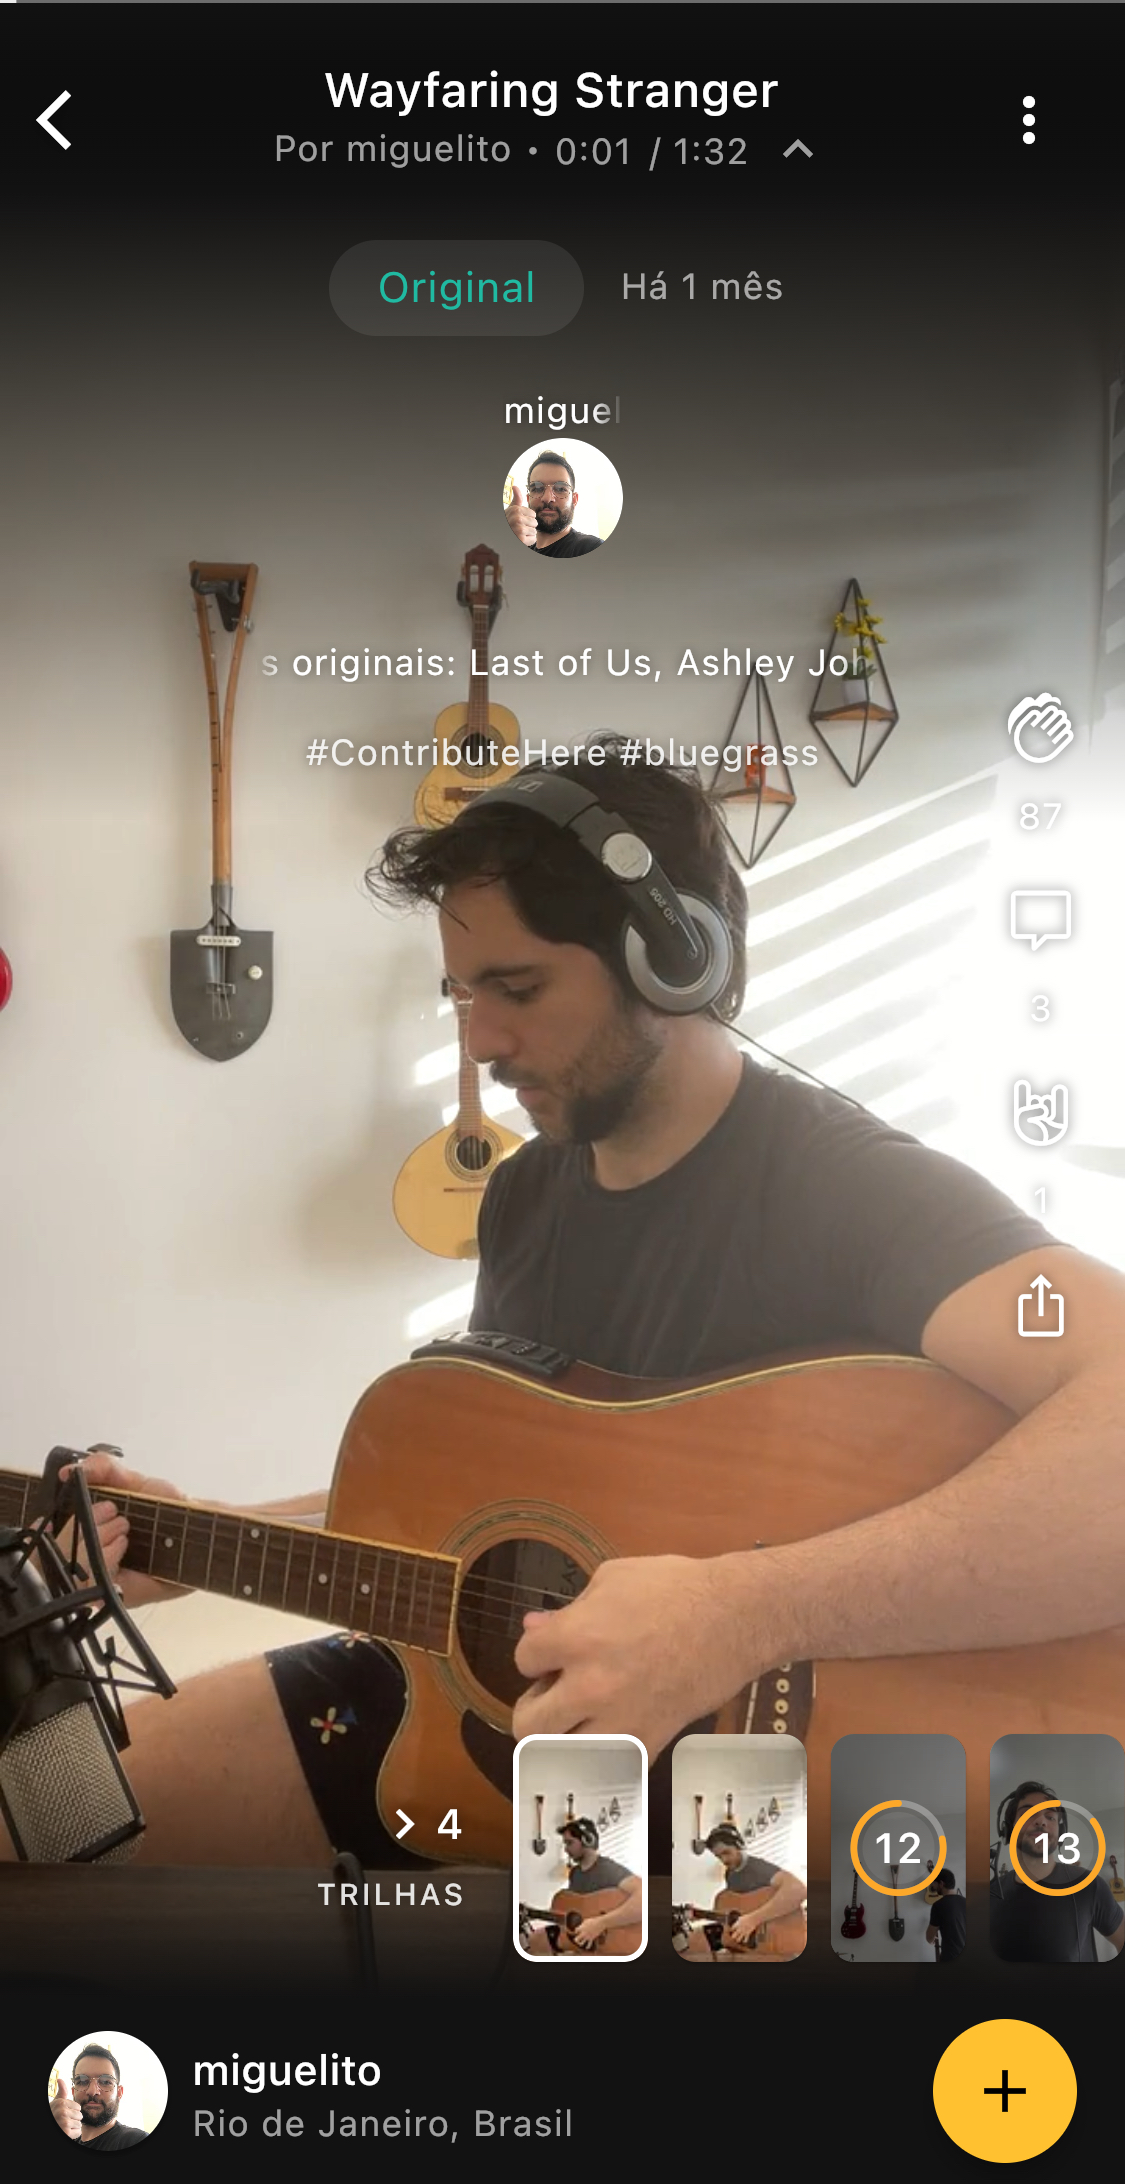
\includegraphics[width=0.4\textwidth]{chapters/chap02/images/wayfaring_original.jpeg}}
    \subfigure[]{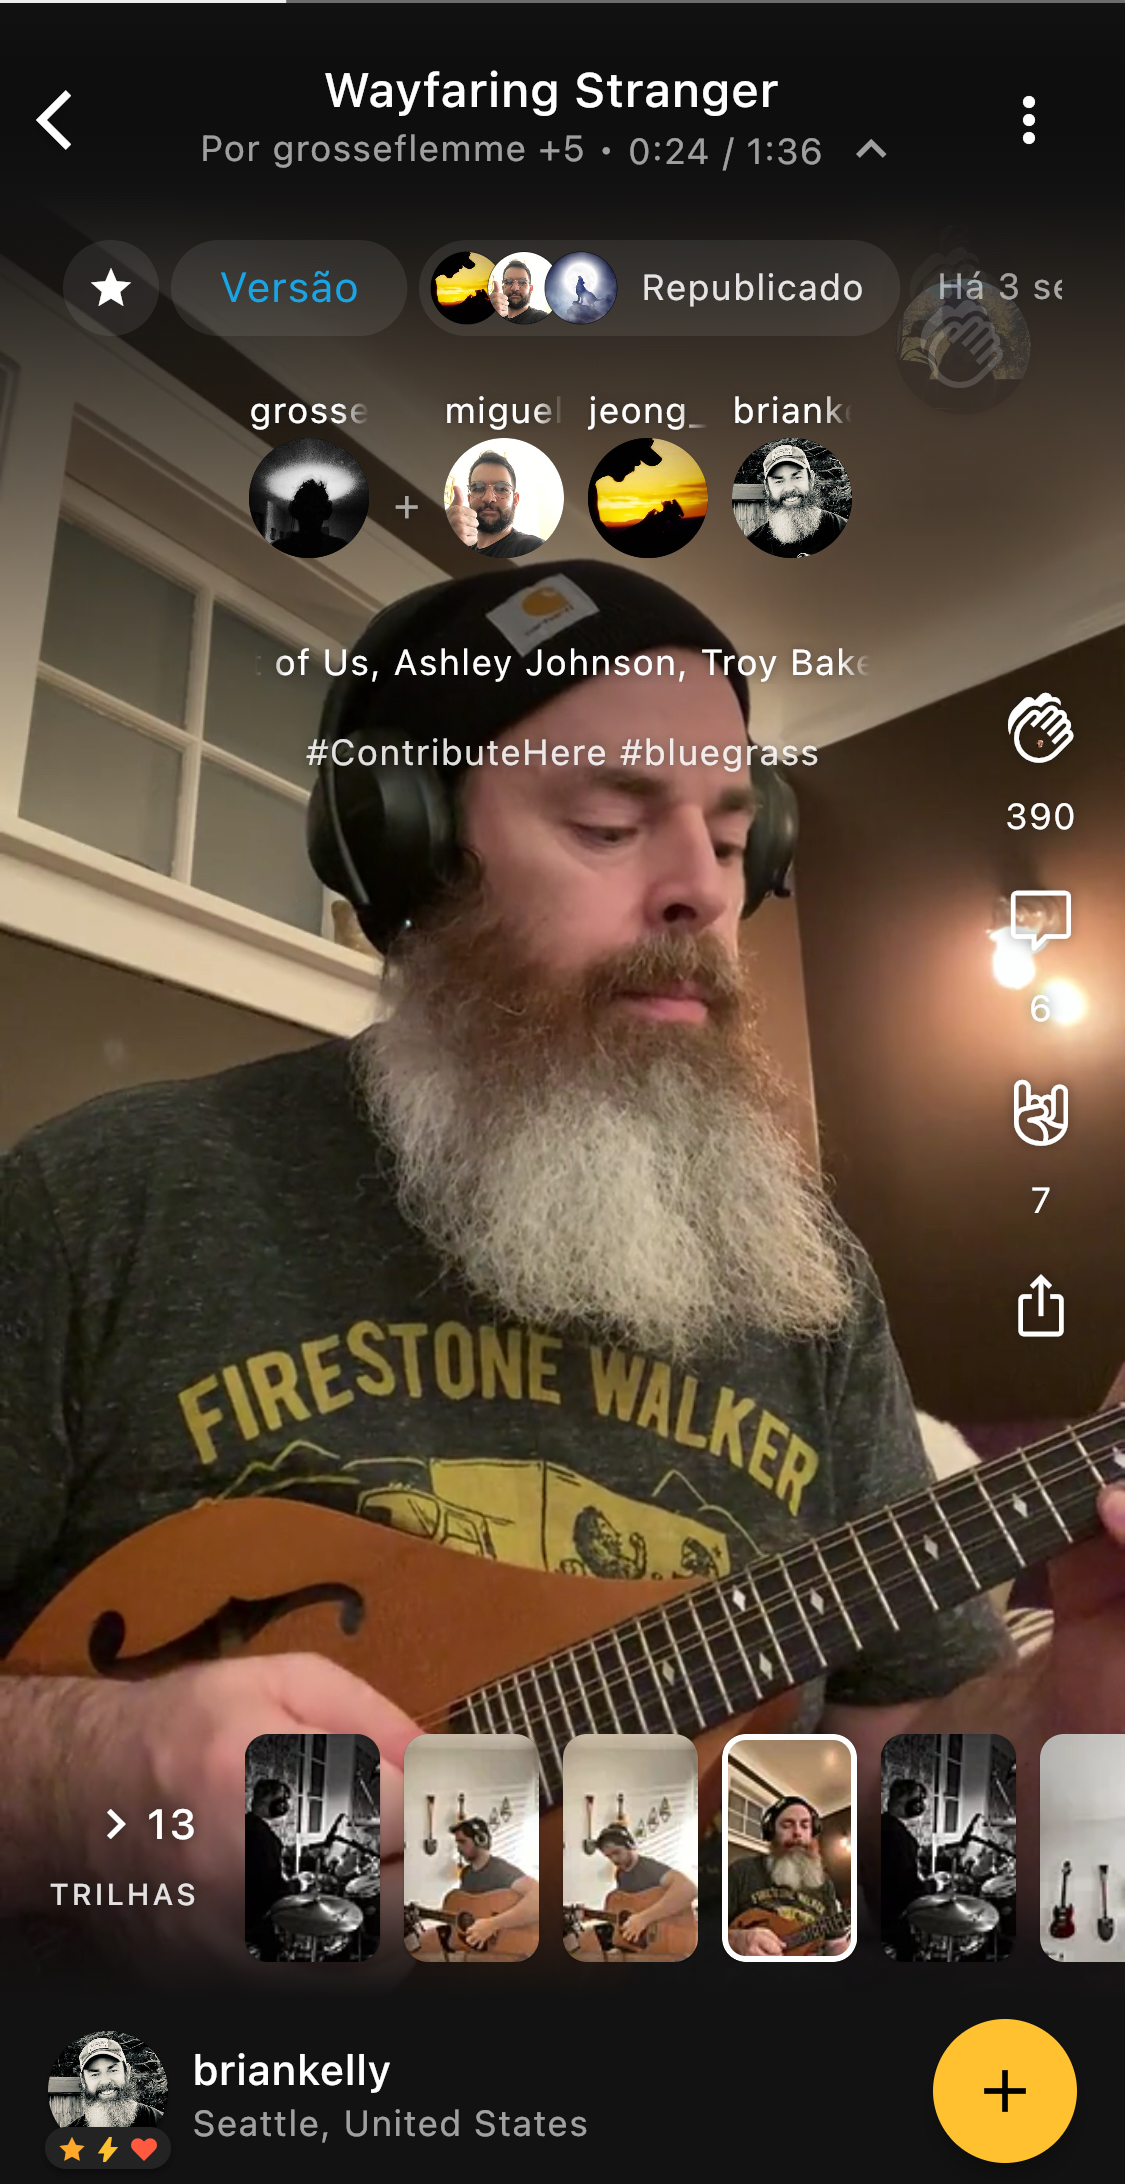
\includegraphics[width=0.4\textwidth]{chapters/chap02/images/wayfaring_fork.jpg}}
    \caption{Duas sessões publicadas no aplicativo Indaband. A primeira sessão é
    a sessão original, enquanto a segunda é um \textit{fork} subsequente da
    primeira. Ambas compartilham o mesmo nome e as faixas da primeira sessão. A
    segunda sessão contém faixas adicionais.}
    \label{fig:session_and_fork}
  \end{center}
  \end{figure}

\subsubsection{\textit{Fork}} Toda sessão publicada disponibiliza a
funcionalidade de \textit{fork} para os demais usuários da plataforma. O
\textit{fork} é uma cópia da sessão original, em que é possível adicionar
gravações inéditas, editar e remover faixas pré-existentes sem afetar a
publicação original. Quando publicada, a sessão \textit{fork} exibe o autor original das faixas
pré-existentes que forem mantidas, além da referência para a sessão anterior.

O \textit{fork} é uma das principais formas de colaboração assíncrona entre
usuários. A FIGURA \ref{fig:session_and_fork} ilustra duas sessões, sendo a
segunda um \textit{fork} subseqeuente da primeira. Note que a quantidade de
faixas e usuários presentes na segunda sessão aumenta. Além disso, conta com
maior quantidade de visualizações, comentários e outras formas de engajamento
positivo. Entre essas duas sessões, houve uma série de \textit{forks}
intermediários, realizados por cada um dos usuários que adicionaram faixas às
suas sessões.


\subsubsection{Faixa}
A faixa é uma mídia com áudio e vídeo que geralmente contém a gravação de um
instrumento ou voz. Uma faixa necessariamente é criada a partir de um entre três
recursos: tal como uma gravação original, tal como um \textit{fork} de uma faixa
publicada anteriormente ou como uma importação de uma mídia de áudio ou de
vídeo.




\section{Sobrecarga de informação}

Após três anos de desenvolvimento, a aplicação conta com dezenas de milhares de
usuários cadastrados, os quais centenas gravam mensalmente. Dado o grande
catálogo de usuários, o processo de encontrar pessoas com interesses musicais
similares demanda tempo e esforço. O mesmo ocorre ao procurar uma sessão que
seja de interesse em meio ao grande volume de conteúdo publicado. Essa
dificuldade percebida pelo usuário é conhecida na literatura de sistemas de
recomendação como sobrecarga de informação \cite{roetzel2019information}.

A sobrecarga de informação, segundo \citet{roetzel2019information}, é um estado em que um tomador de decisões observa um
conjunto ou uma carga de informações de complexidades distintas, a qual inibe a
capacidade do tomador de decisões de determinar de forma ótima a melhor decisão
possível.

\vspace{0.2cm}
\begin{figure}[h]
    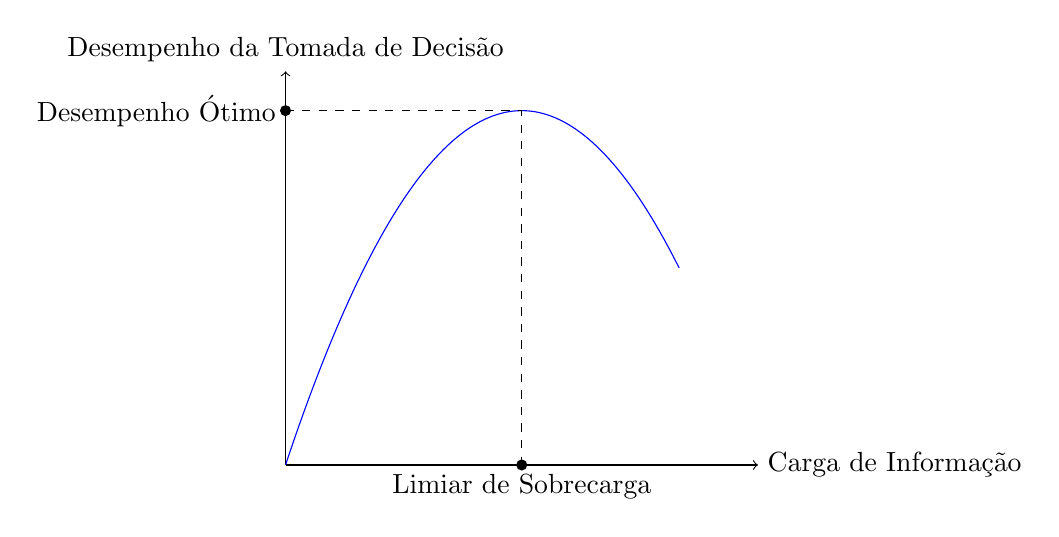
\begin{tikzpicture}
    % Eixo X
    \draw[->] (0,0) -- (6,0) node[right] {Carga de Informação};
    % Eixo Y
    \draw[->] (0,0) -- (0,5) node[above] {Desempenho da Tomada de Decisão};
  
    % Curva U invertida
    \draw[blue, domain=0:5, samples=100] plot (\x, {3*\x - 0.5*\x*\x});
  
    % Pontos de interesse
    \fill (0,4.5) circle (2pt) node[left] {Desempenho Ótimo};
    \fill (3,0) circle (2pt) node[below] {Limiar de Sobrecarga};

    % Linhas tracejadas
    \draw[dashed] (0,4.5) -- (3,4.5);
    \draw[dashed] (3,0) -- (3,4.5);
  \end{tikzpicture}
   % Descrição
    \caption{Correspondência entre a carga de informação e o desempenho da tomada
    de decisão.}
    \label{fig:u_invertida}
\end{figure}
\vspace{0.2cm}

O uso subótimo de informações é causado
pela limitação de recursos individuais escassos. Um recurso escasso pode ser uma
característica individual (como capacidade de processamento em série, memória de
curto prazo) ou equipamento relacionado à tarefa (por exemplo, orçamento ou
tempo para tomar uma decisão). A probabilidade de alcançar a melhor decisão
possível é definida como o desempenho de tomada de decisão. A correspondência
entre a carga de informação e o desempenho da tomada de decisão é ilustrada na
FIGURA \ref{fig:u_invertida} \cite{roetzel2019information}.

Experimentos realizados por \citet{liang2006personalized} mostraram que, ao
avaliar a satisfação de voluntários com um sistema de recomendação de notícias,
a precisão do conteúdo recomendado e o número de itens
recomendados influenciam diretamente na satisfação do usuário, reduzindo a
sobrecarga de informação e a insatisfação gerada pela sobrecarga.

\section{Sistemas de Recomendação}

\abbrev{RS}{sistemas de recomendação}
Sistemas de recomendação (RS, do inglês \textit{recommender systems}) são
ferramentas de \textit{software} que sugerem itens úteis para um usuário, de
acordo com a disponibilidade de seu histórico \cite{ricci2010introduction}. Esses
sistemas, que podem ser personalizados ou não-personalizados, ajudam usuários a
lidarem com processos de tomada de decisão em meio a sobrecarga de informações,
seja na escolha de um produto em um \textit{e-commerce} ou na seleção de um
filme em um serviço de \textit{streaming}. Ao contrário de uma ferramenta de
busca em que o usuário ativamente procura por um item específico, sistemas de
recomendação são úteis quando o usuário explora um catálogo diversificado,
otimizando a distribuição dos itens a partir de suas preferências pessoais. As
FIGURAS \ref{fig:spotify} e \ref{fig:twitter} ilustram sistemas de recomendação
para tarefas distintas: recomendação de \textit{playlists} na plataforma Spotify
e recomendação de perfis de usuário na plataforma Twitter, respectivamente.


\begin{figure}[ht]
    \centering
    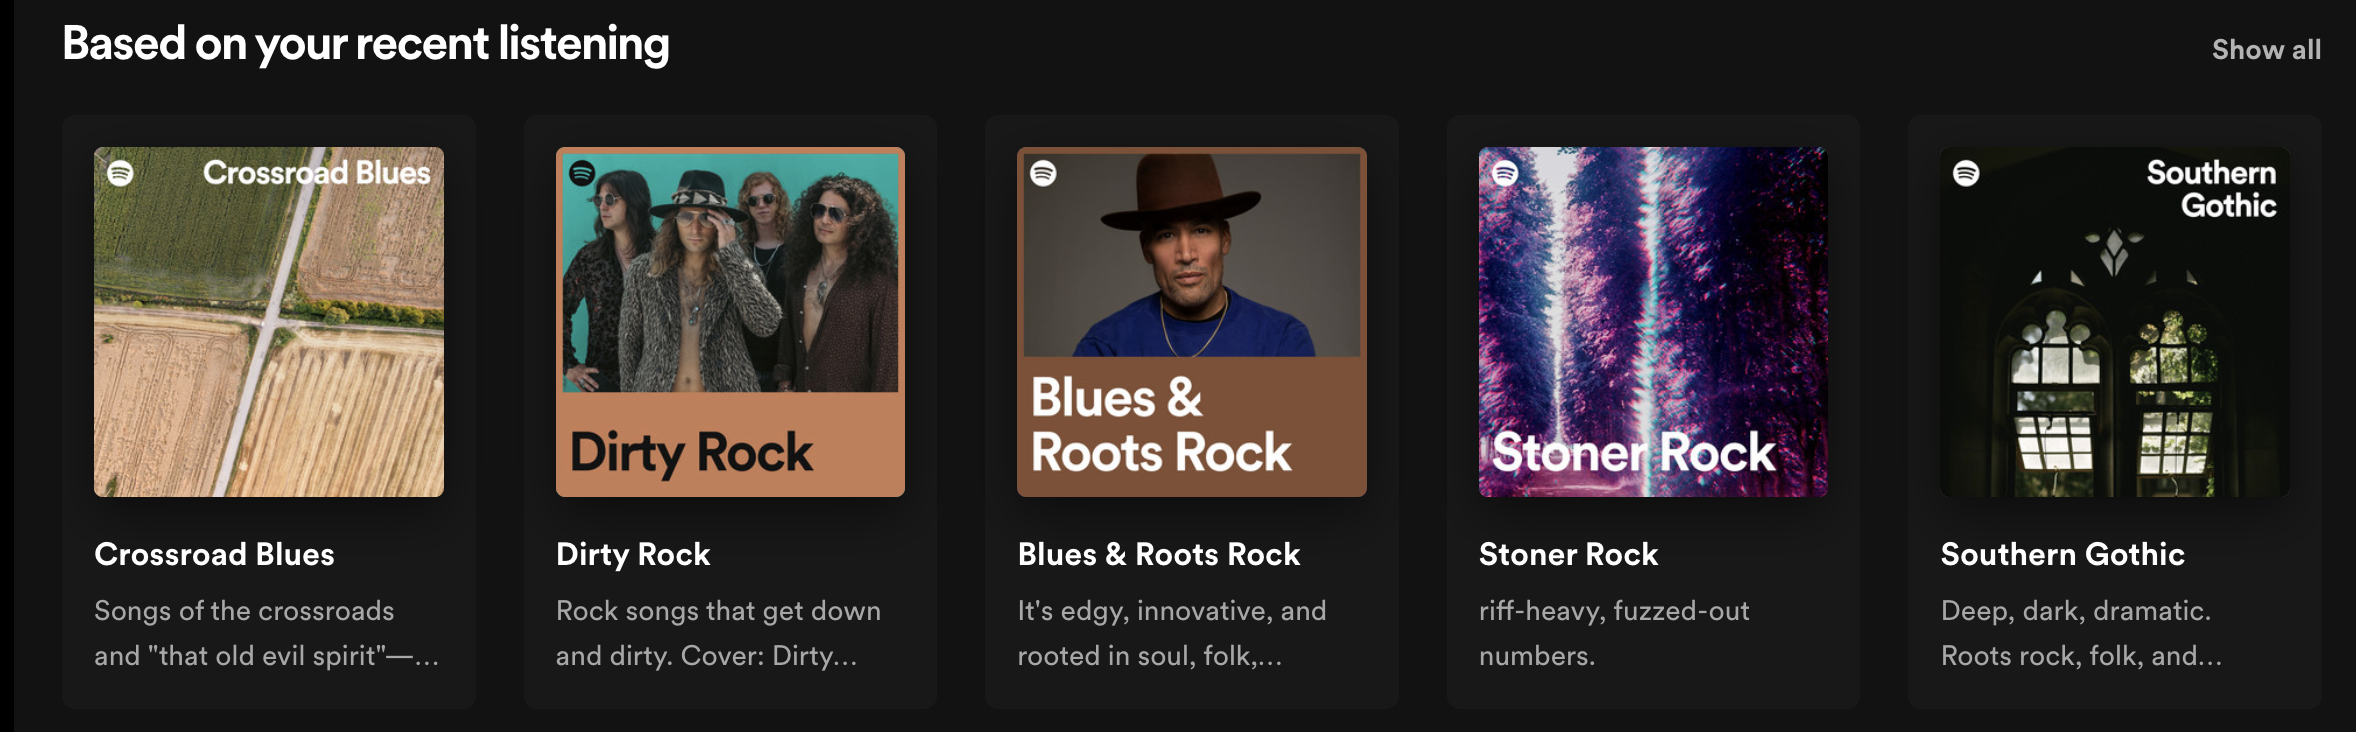
\includegraphics[width=0.8\textwidth]{chapters/chap01/images/spotify.png}
    \caption{Recomendações de \textit{playlists} no Spotify em Agosto de 2023.}
    \label{fig:spotify}
\end{figure}


Personalização é o processo de coleta e uso de informações pessoais para filtrar
conteúdo de forma única a um usuário, atendendo suas necessidades percebidas
pelo serviço ou declaradas explicitamente. \cite{liang2006personalized}.
Recomendações não-personalizadas distribuem o conteúdo recomendado de maneira
igualitária para todos os usuários, desconsiderando suas preferências
individuais. Uma recomendação a partir da lista de reportagens mais lidas em um
portal de notícias é um exemplo de recomendação não-personalizada.
\cite{falk2019practical}.

\begin{figure}[ht]
    \centering
    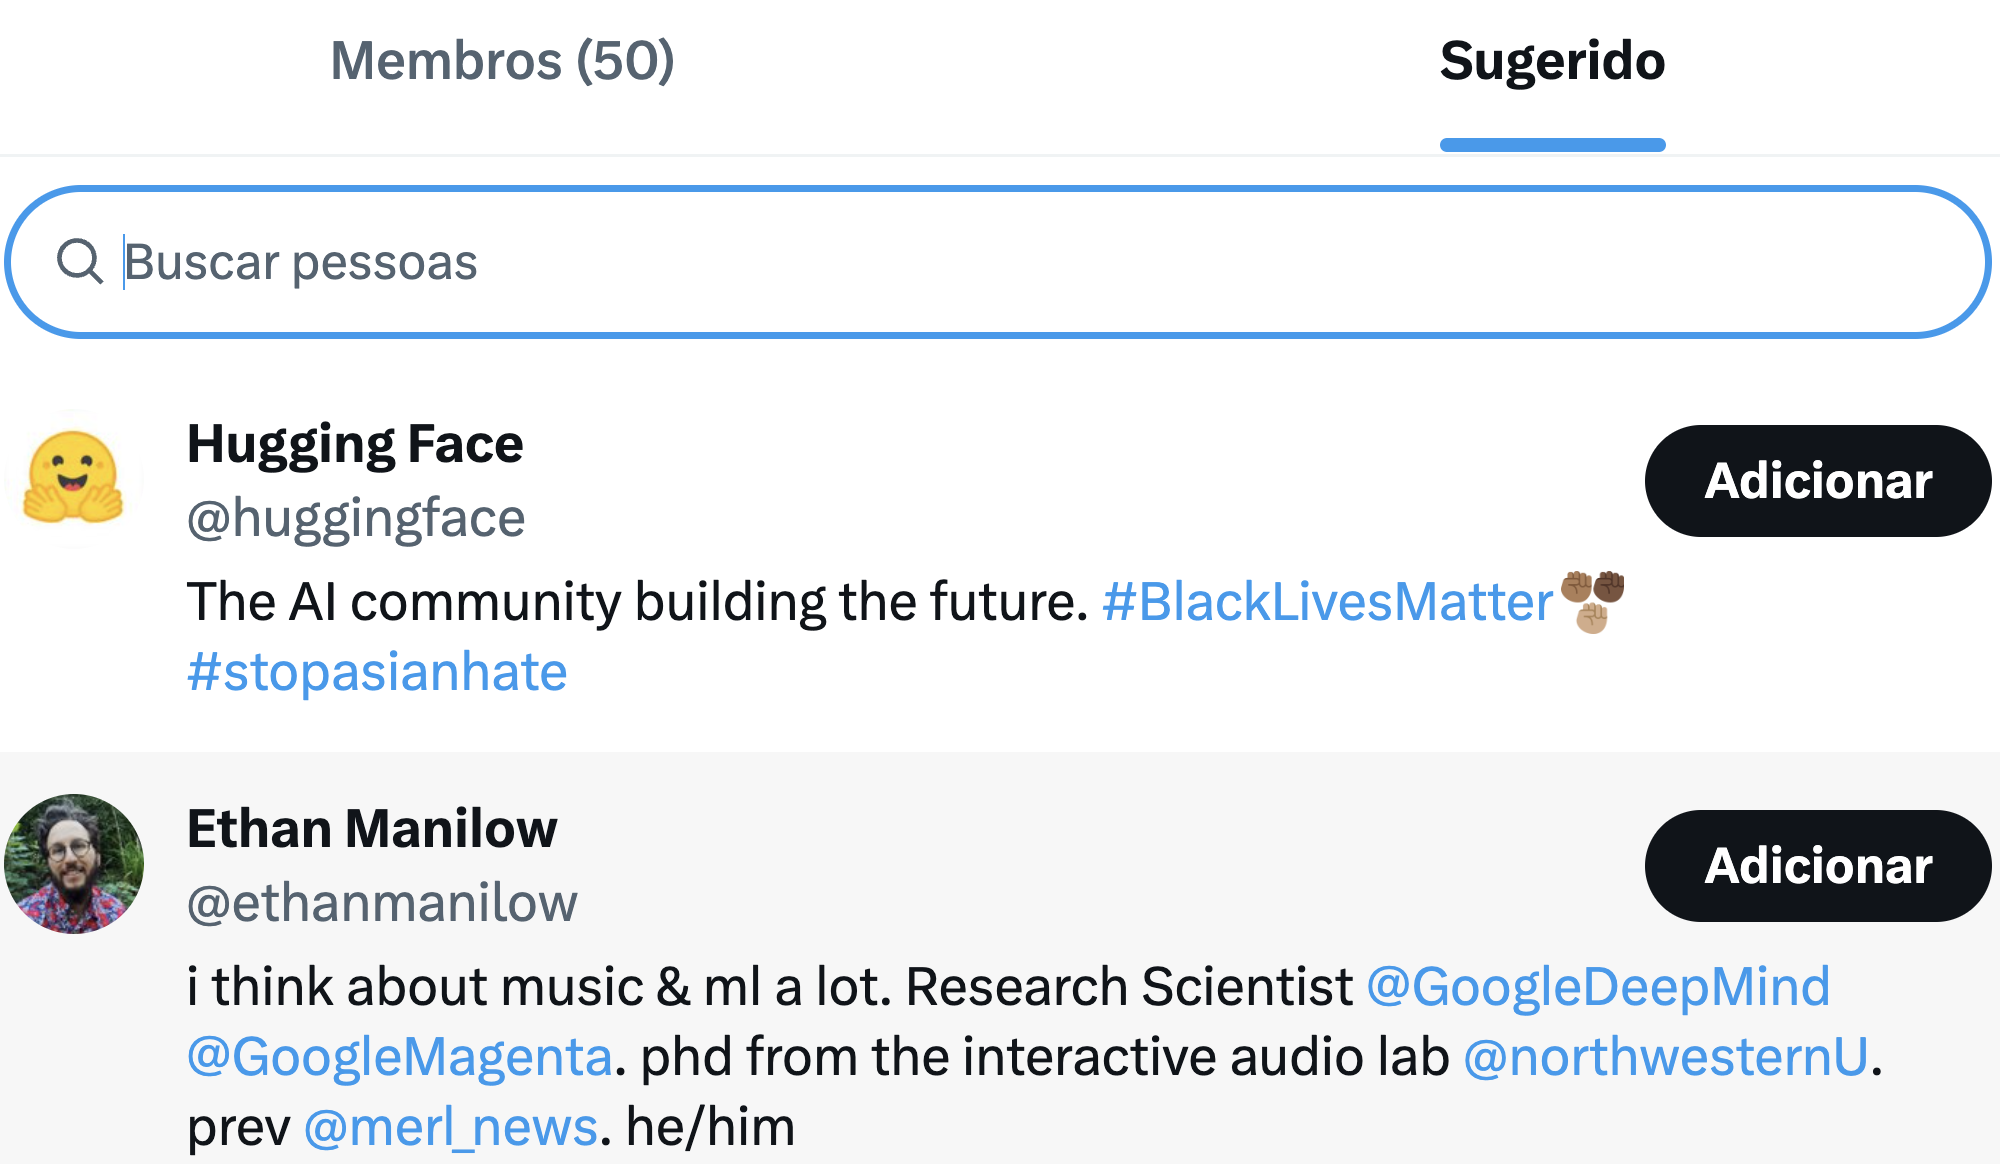
\includegraphics[width=0.6\textwidth]{chapters/chap01/images/tt.png}
    \caption{Recomendações de perfis de usuário no Twitter em Agosto de 2023.}
    \label{fig:twitter}
\end{figure}

% Sistemas de Recomendação Baseados em Sessão (SBRS, do inglês
% \textit{session-based recommender systems}) são sistemas de recomendação que 
Abordagens mais tradicionais em sistemas de recomendação modelam as interações
usuário-item na forma de uma matriz esparsa de avaliações. Cada linha da matriz
representa um usuário e cada coluna representa um item.

A tarefa em questão se
resume ao preenchimento dos valores faltantes da matriz, a depender da
abordagem escolhida. Valores preenchidos com avaliações altas são recomendados
ao usuário, uma vez que ele ainda não os consumiu, tal como ilustrado
na FIGURA \ref{fig:matriz_15}.


\begin{figure}[h]
    \centering
    \begin{tikzpicture}
        % Define the matrix
        \matrix (m) [matrix of nodes,
                    %  nodes in empty cells,
                     column sep=-\pgflinewidth,  % Adjust cell spacing
                     row sep=-\pgflinewidth,     % Adjust cell spacing
                     nodes={draw, text width=2.5em, align=center, minimum height=2.5em, minimum width=2.5em}] {
            5 & 4 & 1 & 1 \\
            4 & 4 & 1 & 1 \\
            1 & 2 &  & 4 \\
            1 & 1 & 4 & 4 \\
        };
      
        % % Labels on the left
        \foreach \row/\label in {1/Gilberto, 2/Maria, 3/Gal, 4/Caetano} {
          \node[left] at (m-\row-1.west) {\label};
        }
      
        % % Labels on the top
        \foreach \col/\label in {1/TV, 2/DVD, 3/sal, 4/pipoca} {
          \node[above,
          ] at (m-1-\col.north) {\label};
        }
      \end{tikzpicture}
      \caption{Matriz de avaliações para produtos de um comércio eletrônico. A predição atua sobre as avaliações não preenchidas.}
      \label{fig:matriz_15}
\end{figure}

\abbrev{SBRS}{Sistemas de recomendação baseados em sessão}
Por mais que a matriz de avaliações seja uma forma intuitiva de representação,
viabilizando uma boa variedade de modelos, trata-se de uma forma que
desconsidera o contexto temporal das interações ou a sequência específica de
itens que determinado usuário interagiu. Sistemas de Recomendação Baseados em
Sessão (SBRS, do inglês \textit{session-based recommender systems}) atuam
justamente nesse cenário.

Os SBRS se caracterizam pelos seus dados representarem um conjunto delimitado de
interações obtidas por \textit{feedback} implícito, ou seja, por preferências
indiretas identificadas a partir de ações ou padrões de navegação. Essas interações
são agrupadas em conjuntos denominados sessões. Uma sessão pode conter uma sequência temporalmente
ordenada de ações executadas por um usuário, ou um conjunto de ações executadas
por um usuário anônimo sem uma ordem específica.

Os objetivos de um SBRS incluem
prever a próxima interação do usuário durante uma sessão em andamento,
recomendar o próximo item ou um conjunto de itens para uma sessão, ou ainda
recomendar uma sessão inteira \cite{domingues_large_2023, survey_wang_2021}.


    



\begin{figure}[h]
    \centering
        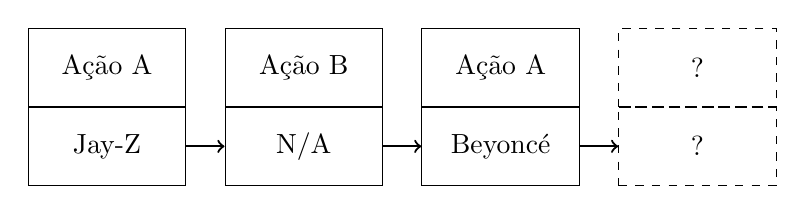
\begin{tikzpicture}
        % Draw the list cells
        \node[draw, rectangle, minimum width=2cm, minimum height=1cm] (cell1) at (0, 0) {Jay-Z};
        \node[draw, rectangle, minimum width=2cm, minimum height=1cm] (cell2) at (2.5, 0) {N/A};
        \node[draw, rectangle, minimum width=2cm, minimum height=1cm] (cell3) at (5, 0) {Beyoncé};
        \node[draw, dashed, rectangle, minimum width=2cm, minimum height=1cm] (cell4) at (7.5, 0) {?};

        % Draw the arrow
        \draw[->, thick] (cell1.east) -- (cell2.west);
        \draw[->, thick] (cell2.east) -- (cell3.west);
        \draw[->, thick] (cell3.east) -- (cell4.west);

        % % Add label to the left of the first cell
        % \node[left] at (cell1.west) {Sessão 1};

        % Draw the top cells with actions
        \node[draw, rectangle, minimum width=2cm, minimum height=1cm] (topcell1) at (0, 1.0) {Ação A};
        \node[draw, rectangle, minimum width=2cm, minimum height=1cm] (topcell2) at (2.5, 1.0) {Ação B};
        \node[draw, rectangle, minimum width=2cm, minimum height=1cm] (topcell3) at (5, 1.0) {Ação A};
        \node[draw, dashed, rectangle, minimum width=2cm, minimum height=1cm] (topcell4) at (7.5, 1.0) {?};

    \end{tikzpicture}
    \caption{Exemplo de uma sessão em andamento.}
    \label{fig:sessao_beyonce}
\end{figure}

Cada interação das sessões está associada a tuplas que contém um ou mais dos
seguintes dados: a ação executada, o item alvo da ação, o instante em que a ação
foi executada e o usuário responsável pela ação. Por exemplo, uma sessão pode
representar uma lista ordenada de itens selecionados por um usuário anônimo, ou
uma lista de ações executadas por usuários de uma mesma sessão, sem que essas
ações estejam necessariamente atreladas cada uma a um item. Isso é um aspecto
útil dos SBRS, por prover recomendações em aplicações em que não há distinção
entre usuários, ou quando as preferências de longo prazo de um usuário novo da
plataforma não foram identificadas. A FIGURA \ref{fig:sessao_beyonce} ilustra um
exemplo de sessão em andamento, em que a ação A corresponde a navegar ao perfil
de determinado artista, enquanto que a ação B corresponde a criar uma
\textit{playlist} vazia. Nem toda ação é necessariamente associada a um item,
como expresso na Ação B.
\vspace{0.4cm}
\section{Trabalhos Futuros}
% TODO: @Miguel - Needs review

A bibliografia existente de espectrograma de modulação, até o presente momento,
aplica uma segunda STFT sobre o domínio acústico, com a finalidade de medir
oscilações de intensidade no eixo da frequência. Dessa forma, o novo eixo obtido
pelo espectrograma de modulação representa modulações de amplitude.

Considerando
que o espectrograma acústico reside em um espaço vetorial $\mathbb{R}_3$, uma proposta de trabalho futuro é
investigar a possibilidade de representar modulações em frequência, bastando que a segunda
STFT meça as oscilações no eixo da frequência para uma dada intensidade
constante.
% \section{Modelagem com inclusão de instrumento e gênero}
\subsection{Base restrita a faixas inéditas} 

Uma característica particular das sessões do Indaband é a capacidade de criar
uma sessão a partir de outra já existente, modificá-la, adicionar novas
gravações e publicá-la como uma nova iteração a partir da funcionalidade de
\textit{fork}.

Essa funcionalidade é muito utilizada pelos usuários. A tabela \ref{tab_sessoes}
mostra que 76\% das faixas criadas são geradas via \textit{fork},
independentemente se foram publicadas ou não. Dessa forma, usuários distintos
podem contribuir para uma mesma sessão em momentos distintos, ou um usuário pode
contribuir para uma mesma sessão de outro usuário que era desconhecido até
então.

Uma vez que o objetivo é recomendar usuários prováveis de contribuir gravando
uma faixa inédita para uma determinada sessão, é razoável gerar um cenário em
que o recomendador seja treinado e avaliado estritamente para prever a próxima
faixa inédita gravada.

As abordagens \textit{next-item} e \textit{remaining-items} são as mais
utilizadas nos comparativos publicados porque aproveitam todos os itens de cada
sessão para o treinamento ou para a avaliação. No caso de uma aplicação em que
haja redundância entre as sessões, em que usuários possam salvar, repetir e
compartilhar sessões entre si, essas abordagens acabam por facilitar o trabalho
do recomendador, uma vez que cada iteração a mais no processo de treinamento
significa uma nova oportunidade para minimizar o erro do modelo. O mesmo vale
para a avaliação, em que identificar faixas \textit{forkadas} seria em tese uma
tarefa mais fácil. O cenário mais desafiador é aquele em que o item a ser
avaliado é necessariamente um item inédito no contexto daquela sessão.

Em contraponto, a abordagem \textit{last-item} é a que mais se aproxima do
cenário mencionado, uma vez que mantém inalterada a sequência de itens das
sessões. O que muda é a forma de avaliação, que passa a considerar apenas o
último item da sequência como o item a ser previsto, sem que os demais itens
anteriores sejam avaliados, minimizando a influência de itens \textit{forkados}
na avaliação.

Com essa finalidade, a base de treinamento do presente trabalho é filtrada:
Nesse último experimento, constam apenas sessões em que o último item da
sequência é a adição de uma faixa inédita. Essa identificação é feita a partir
de um metadado disponível, informando se a faixa foi gerada por um \textit{fork}
ou foi criada, seja por gravação, por importação de uma faixa ou por separação
de fontes.

Para essa abordagem, é utilizado o avaliador \textit{last-item}. Esse avaliador
considera apenas o último item da sequência como o item a ser previsto, sem que
os demais itens advindos de \textit{fork} sejam recomendados.

\begin{table}[htbp]
    \begin{tabular}{|l|l|l|l|l|l|l|l|}
      \hline
      Modelo & HR@5 & HR@10 & MRR@5 & MRR@10 & Cov@10 & Pop@10  \\
      \hline
      GNN & \textbf{0,551} & \textbf{0,625} & \textbf{0,437} & \textbf{0,446} & 0,660 & 0,202  \\
      \hline
      $\text{STAMP}_1$ & 0,519 & 0,584 & 0,377 & 0,386 & 0,610 & 0,217 \\
      \hline
      sknn2 & 0,518 & 0,647 & 0,213 & 0,230 & 0,643 & 0,169 \\
      \hline
      sknn1 & 0,515 & 0,642 & 0,209 & 0,226 & 0,592 & 0,197 \\
      \hline
      ct & 0,509 & 0,579 & 0,390 & 0,399  & 0,477 & 0,349 \\
      \hline
      $\text{STAMP}_2$ & 0,506 & 0,590 & 0,366 & 0,377 & 0,609 & 0,201 \\
      \hline
      $\text{NextItNet}_2$ & 0,465 & 0,563 & 0,341 & 0,354 & 0,566 & 0,249 \\
      \hline
      $\text{STAN}_2$ & 0,464 & 0,596 & 0,178 & 0,196 & 0,547 & 0,179 \\
      \hline
      $\text{STAN}_1$ & 0,451 & 0,572 & 0,186 & 0,202 & 0,529 & 0,177 \\
      \hline
      $\text{NextItNet}_1$ & 0,449 & 0,536 & 0,337 & 0,349 & 0,525 & 0,257\\
      \hline
      vsknn1 & 0,447 & 0,580 & 0,1193 & 0,211 & 0,544 & 0,208 \\
      \hline
      $\text{VSTAN}_1$ & 0,441 & 0,580 & 0,180 & 0,198 & 0,507 & 0,221 \\
      \hline
      $\text{SMF}_2$ & 0,439 & 0,553 & 0,291 & 0,306 & 0,306 & 0,240 \\
      \hline
      $\text{SMF}_1$ & 0,431 & 0,530 & 0,298 & 0,311 & 0,240 & 0,257 \\
      \hline
      vsknn2 & 0,427 & 0,564 & 0,172 & 0,190 & 0,618 & 0,163 \\
      \hline
      $\text{SR}_2$ & 0,423 & 0,534 & 0,277 & 0,291 & 0,471 & 0,238 \\
     \hline
      $\text{VSTAN}_2$ & 0,418 & 0,546 & 0,171 & 0,189 & 0,588 & 0,142 \\
      \hline
      $\text{SR}_1$ & 0,410 & 0,512 & 0,279 & 0,292 & 0,445 & 0,259 \\
      \hline
      ar & 0,395 & 0,498 & 0,248 & 0,262 & 0,454 & 0,265 \\
      \hline 
      $\text{NARM}_1$ & 0,361 & 0,455 & 0,229 & 0,241 & 0,658 & 0,199 \\
      \hline
      $\text{NARM}_2$ & 0,324 & 0,440 & 0,211 & 0,226 & 0,665 & 0,188 \\
      \hline
      FOSSIL & 0,287 & 0,420 & 0,137 & 0,154 & 0,776 & 0,249 \\
      \hline
      FPMC & 0,281 & 0,419 & 0,124 & 0,143 & 0,764 & 0,241 \\
      \hline
      FISM & 0,275 & 0,434 & 0,120 & 0,141 & 0,749 & 0,240 \\
      \hline
      BPRMF & 0,271 & 0,407 & 0,122 & 0,141 & 0,744 & 0,250 \\
      \hline
      CSRM & 0,264 & 0,343 & 0,158 & 0,168 & 0,596 & 0,137  \\ 
      \hline
      $\text{GRU4Rec}_2$ & 0,208 & 0,278 & 0,130 & 0,139 & 0,873 & \textbf{0,030}  \\
      \hline
      $\text{GRU4Rec}_1$ & 0,195 & 0,271 & 0,123 & 0,134 & \textbf{0,858} & 0,040  \\
      \hline
      rpop & 0,165 & 0,225 & 0,106 & 0,113 & 0,009 & 0,319 \\
      \hline
      pop & 0,127 & 0,242 & 0,083 & 0,098 & 0,006 & 0,530 \\
      \hline
      spop & 0,125 & 0,219 & 0,059 & 0,071 & 0,299 & 0,471 \\
      \hline
      random & 0,003 & 0,005 & 0,001 & 0,001 & 1,000 & 0,014 \\
      \hline
      \end{tabular}
      \label{tab:results_last_item_final}
    \caption{Resultado dos modelos \textit{session-based} na abordagem
    \textit{single item}, avaliando o último item da sessão. Modelos ordenados por HR@5. }
  \end{table}

  A tabela \ref{tab:results_last_item_final} mostra os resultados obtidos pela
  abordagem \textit{last-item}. As métricas obtiveram valores na mesma faixa da
  abordagem \textit{next-item}, demonstrando que, por mais que a avaliação e o
  treinamento seja reservados apenas ao último item da sequência, os modelos
  mantém desempenho equivalente.
  
  Novamente, o modelo GNN obteve os melhores resultados. Modelos
  mais simples, como o skNN e a árvore de contexto também obtiveram bons
  resultados.





  %%________________________

  %%________________________
  %% CHAPTER 02
  \chapter{Fundamentação Teórica}
\section{Correspondência entre inteligibilidade e modulação}


 

% Nervo Auditivo:
% - resolução em frequência e resposta da modulação
% - diversidade de resposta
% - caracteristica passa baixa das fibras do nervo auditivo
% - faixa dinâmica

% Nucleo coclear:
% - resolução em frequência e resposta da modulação
% - diversidade de resposta
% - caracteristica passa baixa das fibras do nervo auditivo
% - faixa dinâmica

% A audição humana pode ser aproximada por um filtro
%  passa-baixas.\cite{langner1992}.

% Modulações abaixo de 20Hz são percebidas ritmicamente. Modulações predominantes
% entre 3 e 4Hz coencidem com a taxa que pronunciamos palavras. \cite{langner1992}.

% Modulações entre 10Hz e 200Hz são percebidas como desagradáveis. \cite{langner1992}.

% \cite{langner1992} define a percepção de periodicidade do envelope como 
% "periodicity pitch". 

% MTF: modulation transfer function.

% A percepção de pitch trata da frequência percebida. Dois sinais complexos
% compostos por diversas componentes frequênciais distintas podem ter o mesmo
%  pitch. Ainda, um sinal, por mais que tenha determinado pitch, pode não conter essa
%  frequência em sua composição. A percepção de pitch funciona por mais que não esteja presente a 
%  frequência fundamental de mesmo valor daquele pitch. \cite{langner1992}

%  Nervo auditivo. Núcleo Coclear. \cite{langner1992}.

%  This indicates that the auditory system tends to separate information about
%   the envelope and the temporal fine structure of a signal as
%    a first step of temporal analysis of sounds.


% Efeito do envelope na percepção de fala:

% \cite{drullman1994} O sinal de fala é caracterizado por um espectro de
%  frequências variante no tempo. Essas variações são responsáveis pela
%  identificação de fonemas, sílabas, palavras e frases.

%  Em todas as bandas, as frequências mais importantes são as presentes entre
%  3 e 4 Hz, refletindo a taxa silábica da fala. É possível encontrar componentes
%  na faixa entre 15-20hz.

%  A sensibilidade para modulação tem caracteristica de um filtro passa-baixa,
%  com queda de 6dB entre 25Hz e 100Hz.

%  Posso colocar um gráfico aqui. Como que se mede esse gráfico?

%  MI: Modulation Index.
%  SRT: Speech-Reception Threshold.
%  STI: Speech-Transmition Index.

%  Em áudio reverberante, a atenuação da modulação diminiu a inteligibilidade de 
%  frases. \cite{drullman1994}. Compressão, por subbandas ou diretamente no sinal,
%  afeta drasticamente a inteligibilidade.

%  Essa informação é útil para síntese de voz? Dado que eu quero sintetizar
%  uma voz com inteligibilidade alta. E para análise do som, em aparelhos para
%  deficientes auditivos?

%  O efeito de borramento é reproduzido em áudio reverberante, ao convoluir
%  um sinal com uma exponencial que decai.

%  Pode ser medida em termos de matriz de confusão.

%  SIQ (sentence intelligibility in quiet).

%  Qual a tradução de smearing? Achatamento, borramento, espalhamento?

%  Detecção de envelope com transformada de Hilbert.
 
% Consoantes são mais afetadas por borramento temporal do que vogais.
\section{Cicloestacionariedade de Segunda Ordem e de Ordem Superior}

\section{Correspondência entre inteligibilidade e modulação}
\section{Speech Enhancement}
˜\newpage 
˜\newpage
\section{STFT}
\newpage 
˜\newpage 
\section{Framework AMS}
\newpage 
˜\newpage 
\section{Espectrograma de modulação}
\newpage 
˜\newpage 
˜\newpage
  %%________________________

   %%________________________
  %% CHAPTER 03
  \chapter{Fundamentação Teórica}
\section{Indaband}
A música, enquanto atividade e produto, permite o estabelecimento de laços sociais
entre musicistas e ouvintes.

A atividade musical permite que um conjunto de musicistas interaja e
comunique-se, facilitada quando os membros compartilham de uma mesma bagagem
cultural. Além disso, permite que a audiência estabeleça um vínculo com
o músico executor ou o conjunto de musicistas \cite{cook2021music}.

Por sua vez, a música enquanto produto permite o estabelecimento de laços sociais
entre os ouvintes, seja em uma sala de concerto no século XIX, em uma sala de estar
com um rádio ou um gramofone no século XX, ou em uma apresentação ao vivo na
plataforma Twitch no século XXI.

Durante a pandemia de COVID-19, estudantes de música precisaram adaptar seus
hábitos de prática musical para aulas remotas e práticas individuais. A prática
coletiva foi fortemente afetada, uma vez que as aulas e os ensaios presenciais
foram suspensos em uma série de instituições de ensino, dado o risco de
contaminação e a necessidade de distanciamento social \cite{nusseck2021musical}.

A prática remota síncrona, hoje, enfrenta uma série de desafios técnicos. A
latência entre os praticantes é o principal problema. O limiar da percepção
auditiva para atrasos é de cerca de 20 milissegundos, enquanto que sistemas VoIP
com latência de 150 milissegundos e \textit{jitter} de 30 milissegundos são
considerados de boa qualidade. A codificação associada à compressão do sinal e a
largura de banda também influenciam no atraso. Enquanto a latência em uma
comunicação instantânea não for inferior ao limiar da percepção, essa forma de
prática musical não será viável.

A principal alternativa é a prática musical colaborativa assíncrona. Nesse
cenário, cada praticante grava sua faixa de forma individual enquanto ouve as
demais faixas gravadas. Aplicações como \textit{BandLab}, \textit{Ableton Live}
e \textit{Soundtrap by Spotify} funcionam sob essa abordagem.

Uma segunda característica da prática musical coletiva, seja no contexto
presencial ou remoto, é a necessidade de encontrar outros interessados com
gostos musicais similares, instrumentos que se complementem, etc. Uma pessoa que
deseja tocar um estilo musical específico, incomum na região em que vive,
sofreria dessa dificuldade. Um meio de resolver esse problema é recorrer à
comunidades virtuais ou redes sociais. Ao encontrar outros interessados, caso a
distância impeça a prática presencial, a atividade pode ser realizada a partir
da prática musical colaborativa assíncrona. Plataformas como \textit{Cifra Club}
e \textit{Ultimate Guitar} permitem que usuários contribuam com tablaturas de
músicas e comentários, formando uma comunidade virtual.


Tanto a prática musical colaborativa assíncrona quanto a formação de comunidades
virtuais de música são problemas os quais o mercado oferece poucas soluções
integradas. Estações de trabalho de áudio digital (DAWs, do inglês
\textit{Digital Audio Workstations}) mais tradicionais, como \textit{Pro Tools},
\textit{Logic Pro} e \textit{Ableton Live} são desprovidos de funcionalidades de
interação social. \textit{Cifra Club} e \textit{Ultimate Guitar} não permitem a
gravação colaborativa de forma assíncrona. \textit{Soundtrap by Spotify} e
\textit{BandLab} permitem a edição colaborativa em tempo real, porém apenas o
último contém funcionalidades de interação e integração social entre usuários. A
aplicação \textit{Collab}, da Meta, preenchia parcialmente esses critérios antes
de ser descontinuada. O aplicativo móvel Indaband foi criado para ocupar esse
espaço pouco preenchido no mercado.

\begin{figure}[h]
    \centering
    \subfigure[]{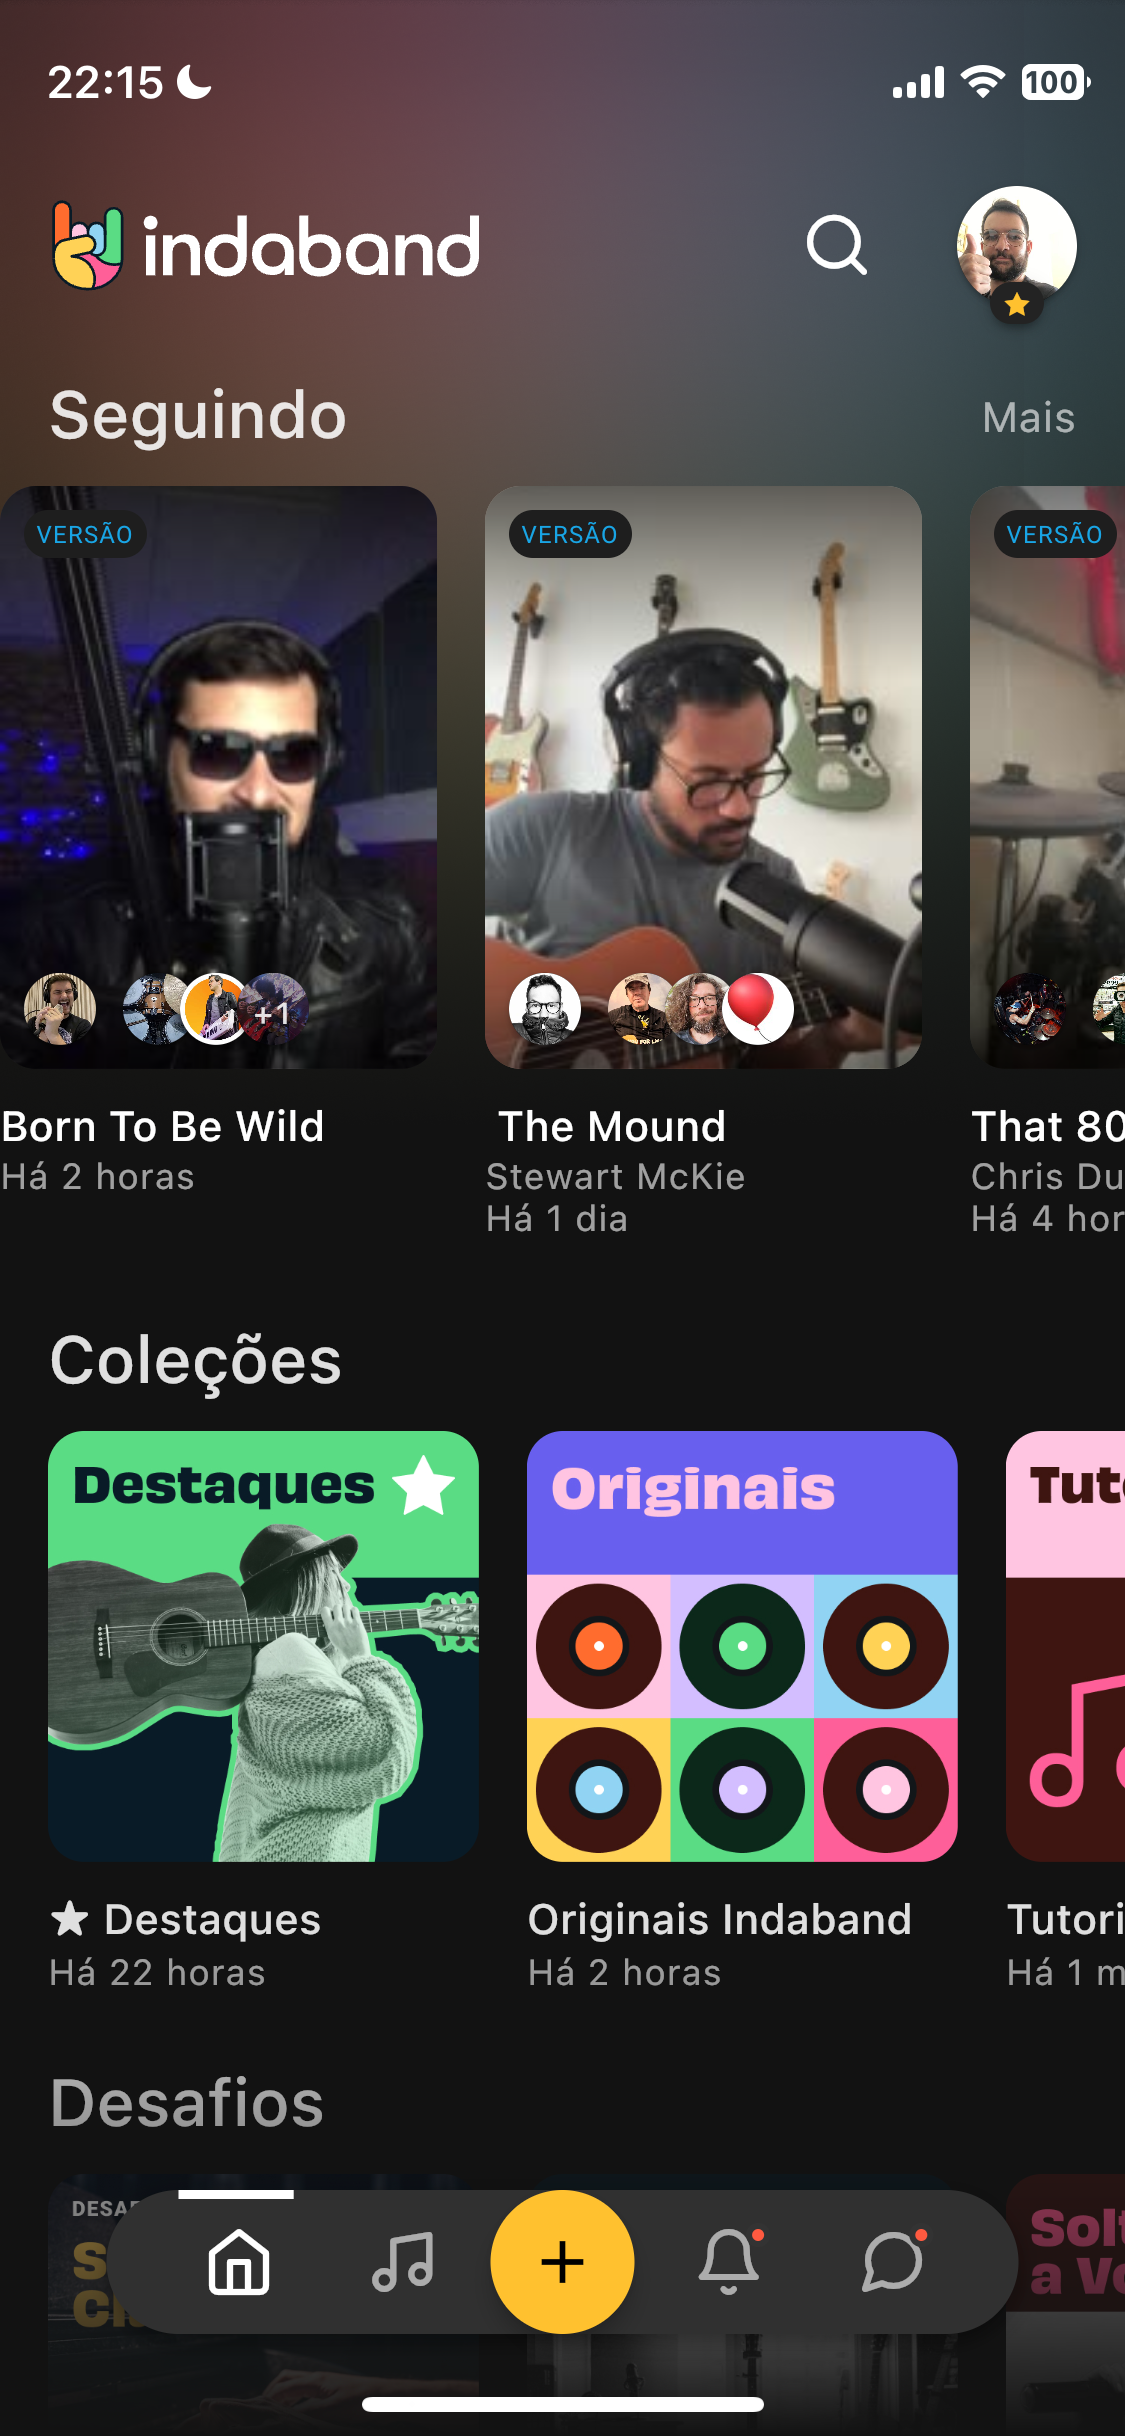
\includegraphics[width=0.24\textwidth]{chapters/chap01/images/inda/inda3.PNG}}
    \subfigure[]{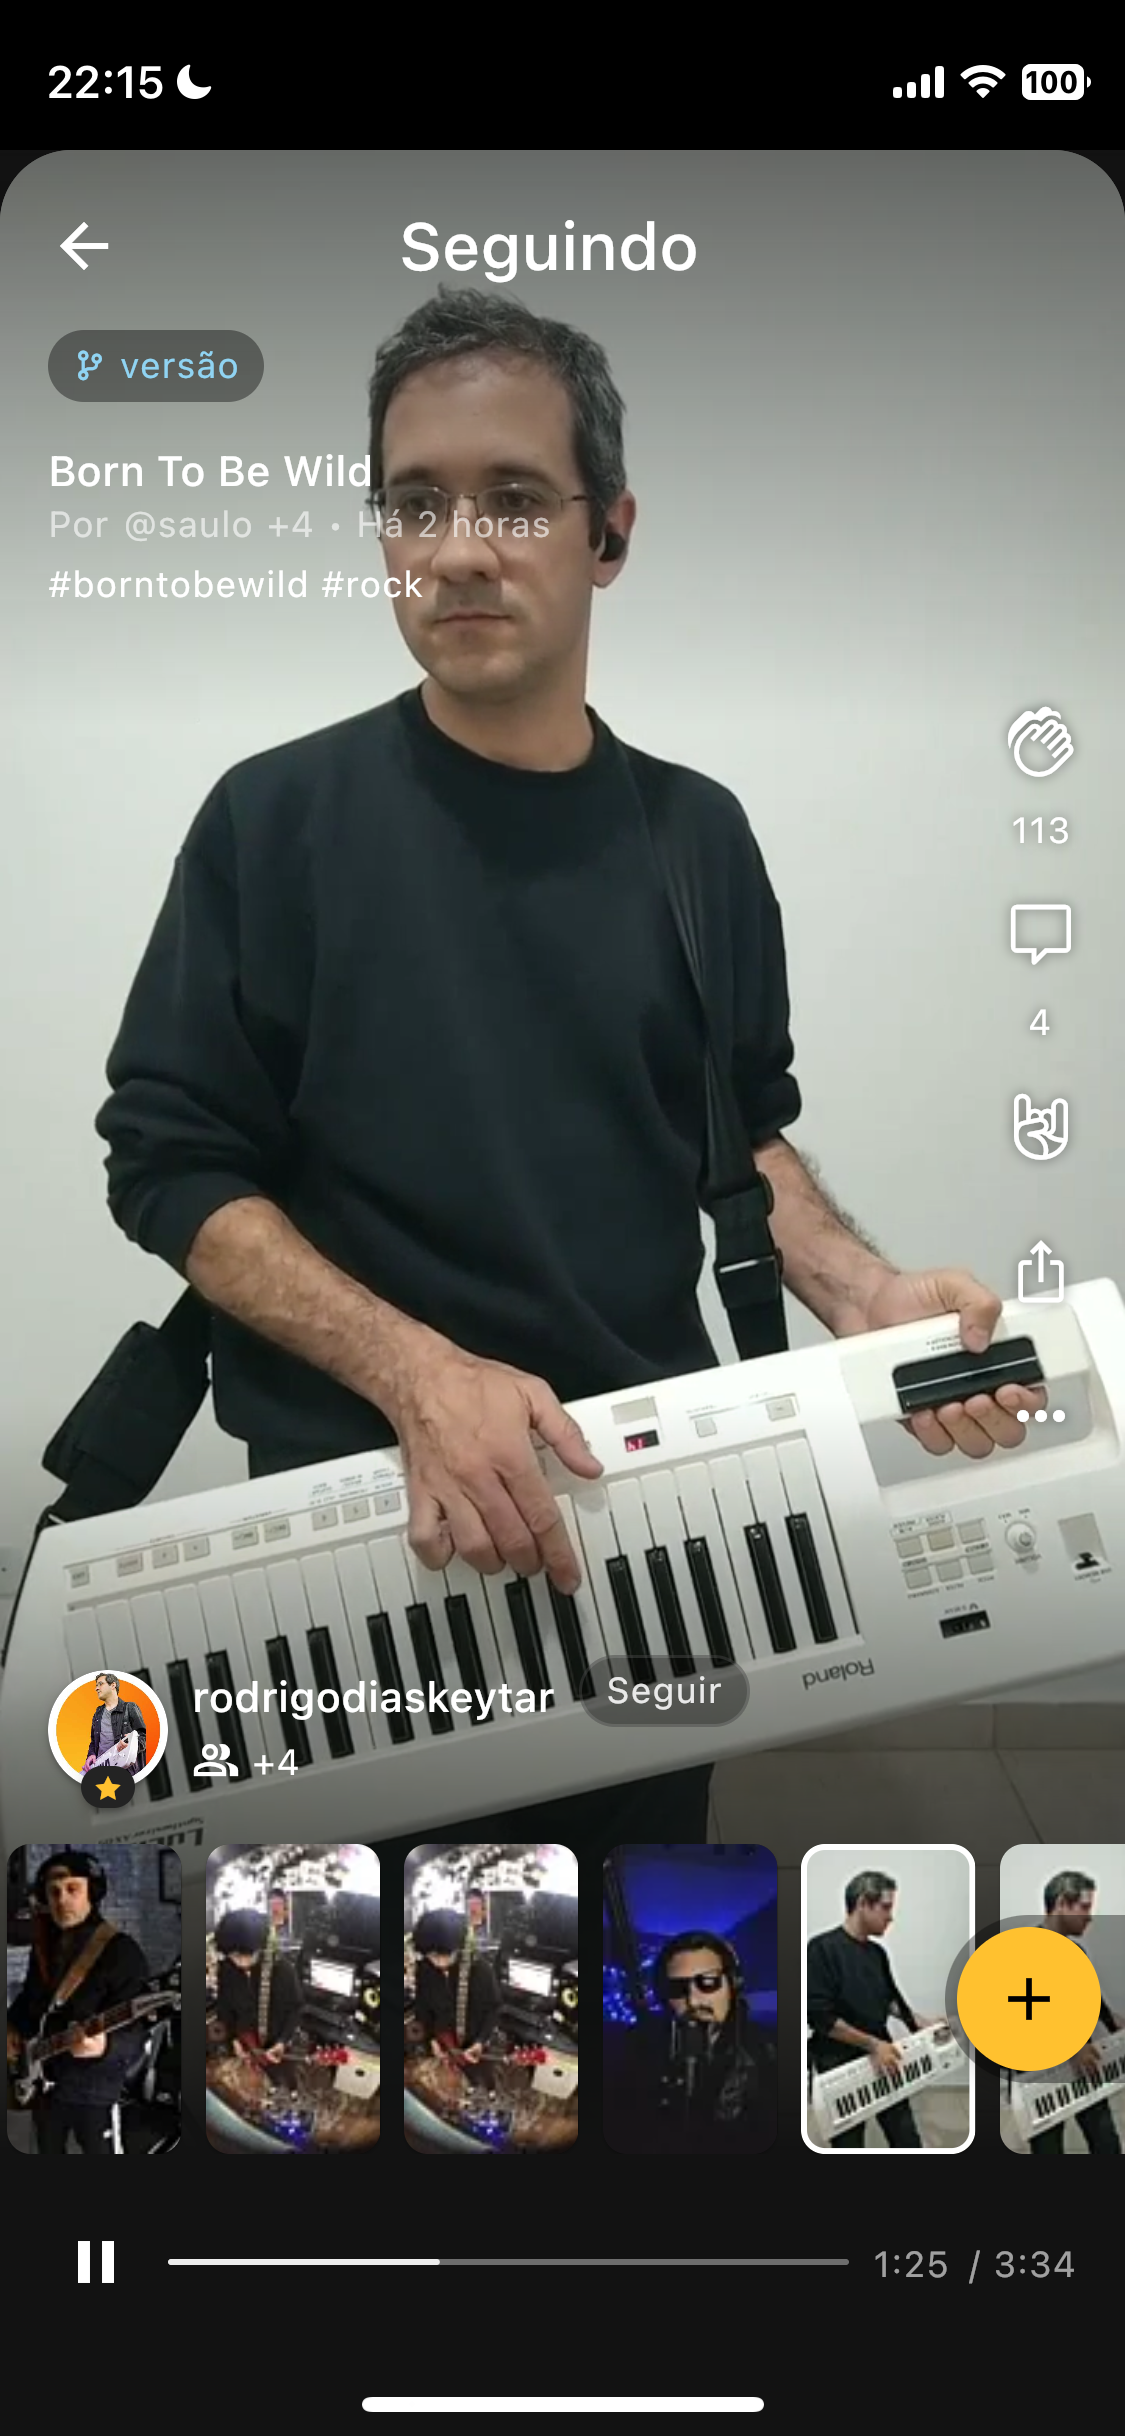
\includegraphics[width=0.24\textwidth]{chapters/chap01/images/inda/inda.PNG}}
    \subfigure[]{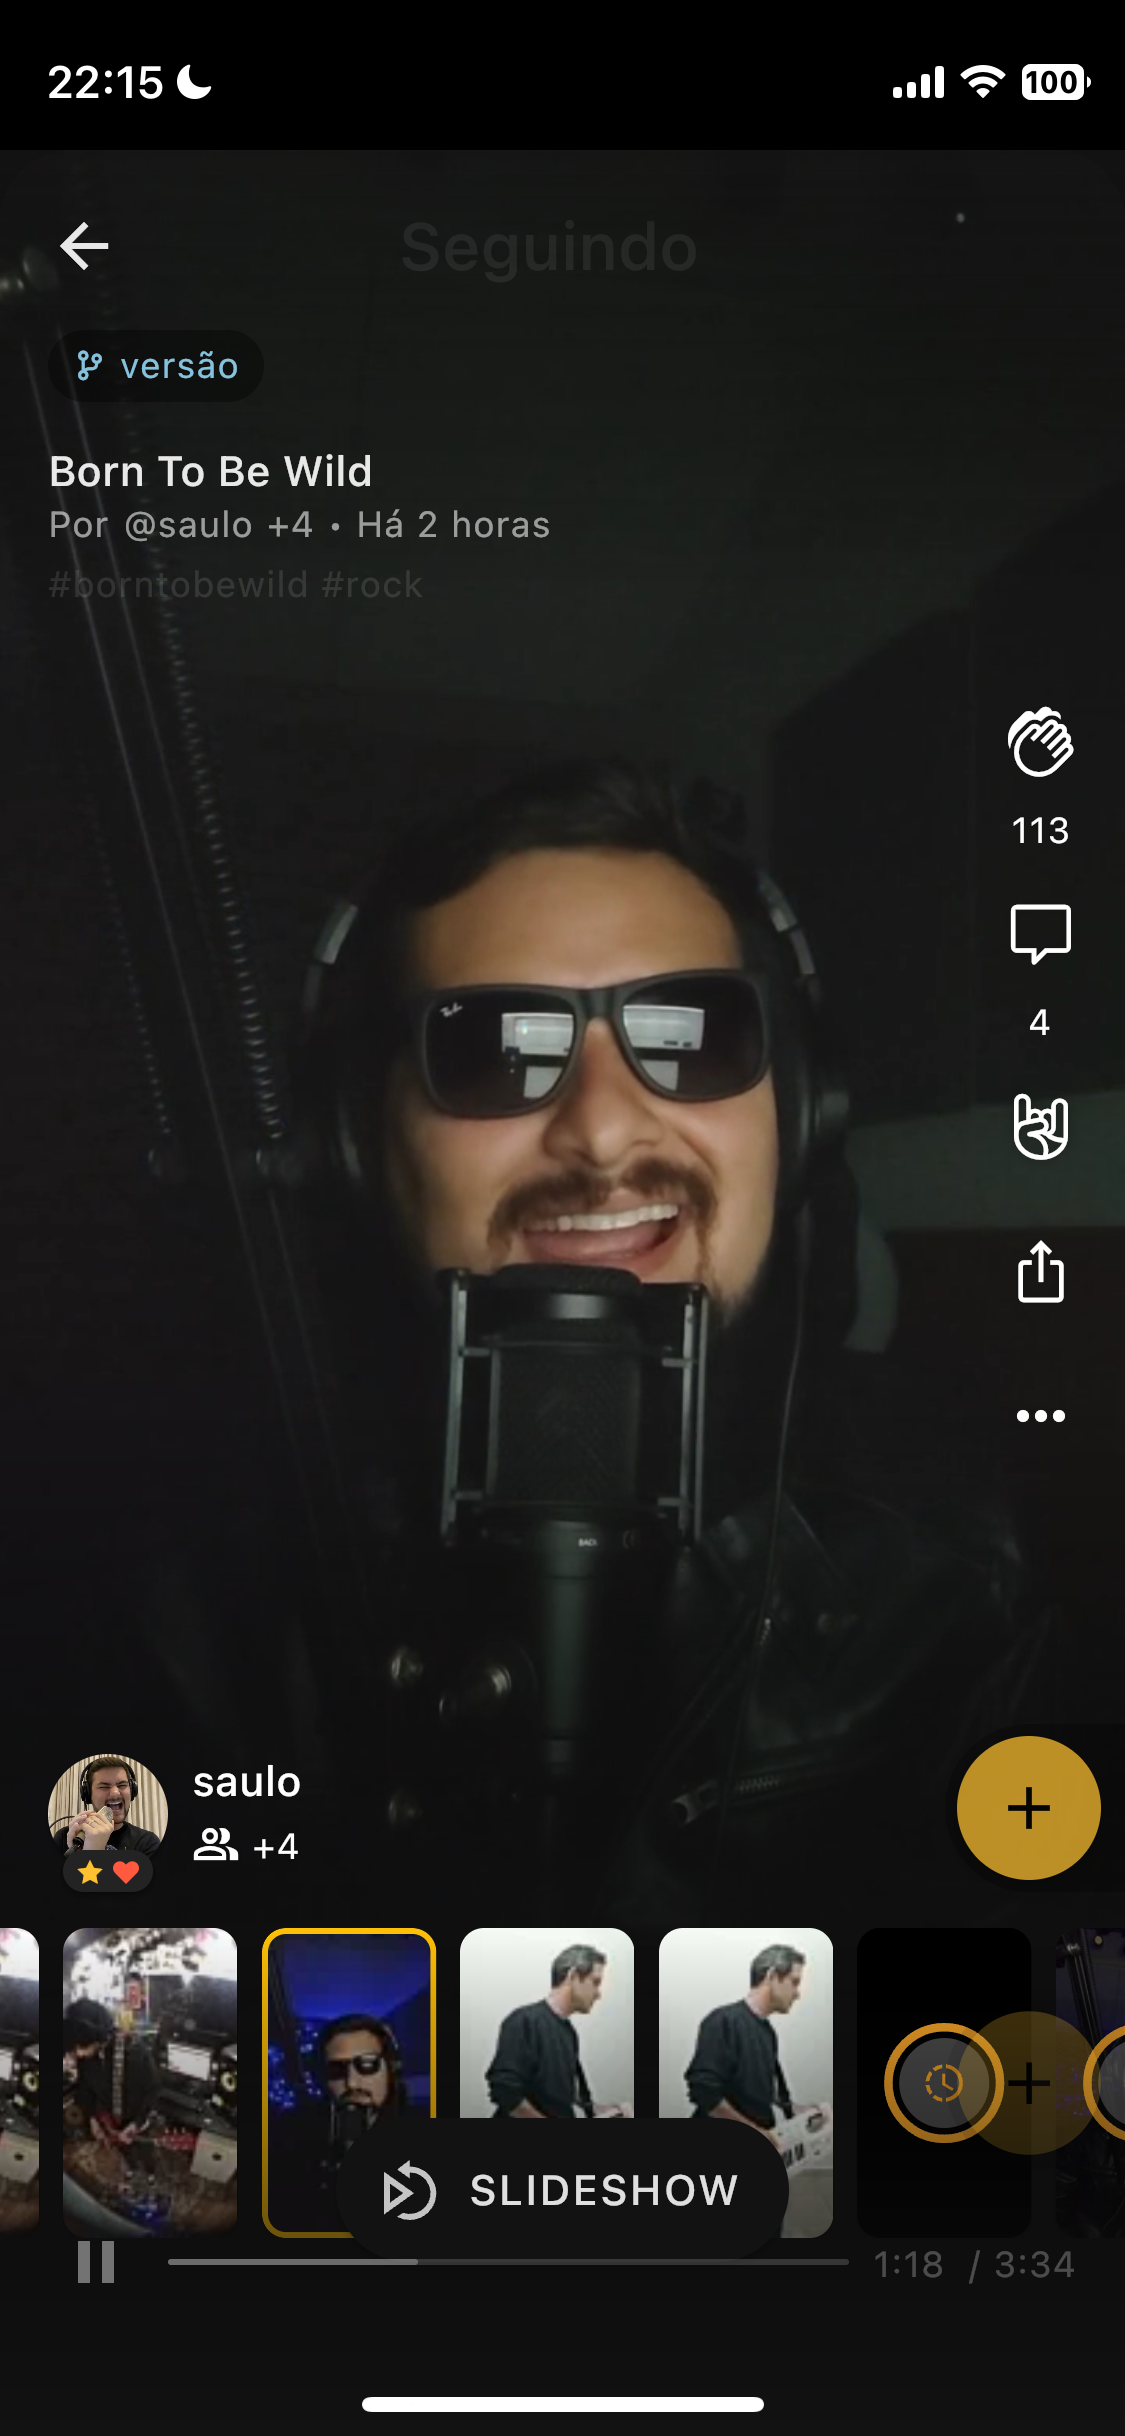
\includegraphics[width=0.24\textwidth]{chapters/chap01/images/inda/inda2.PNG}}
    \subfigure[]{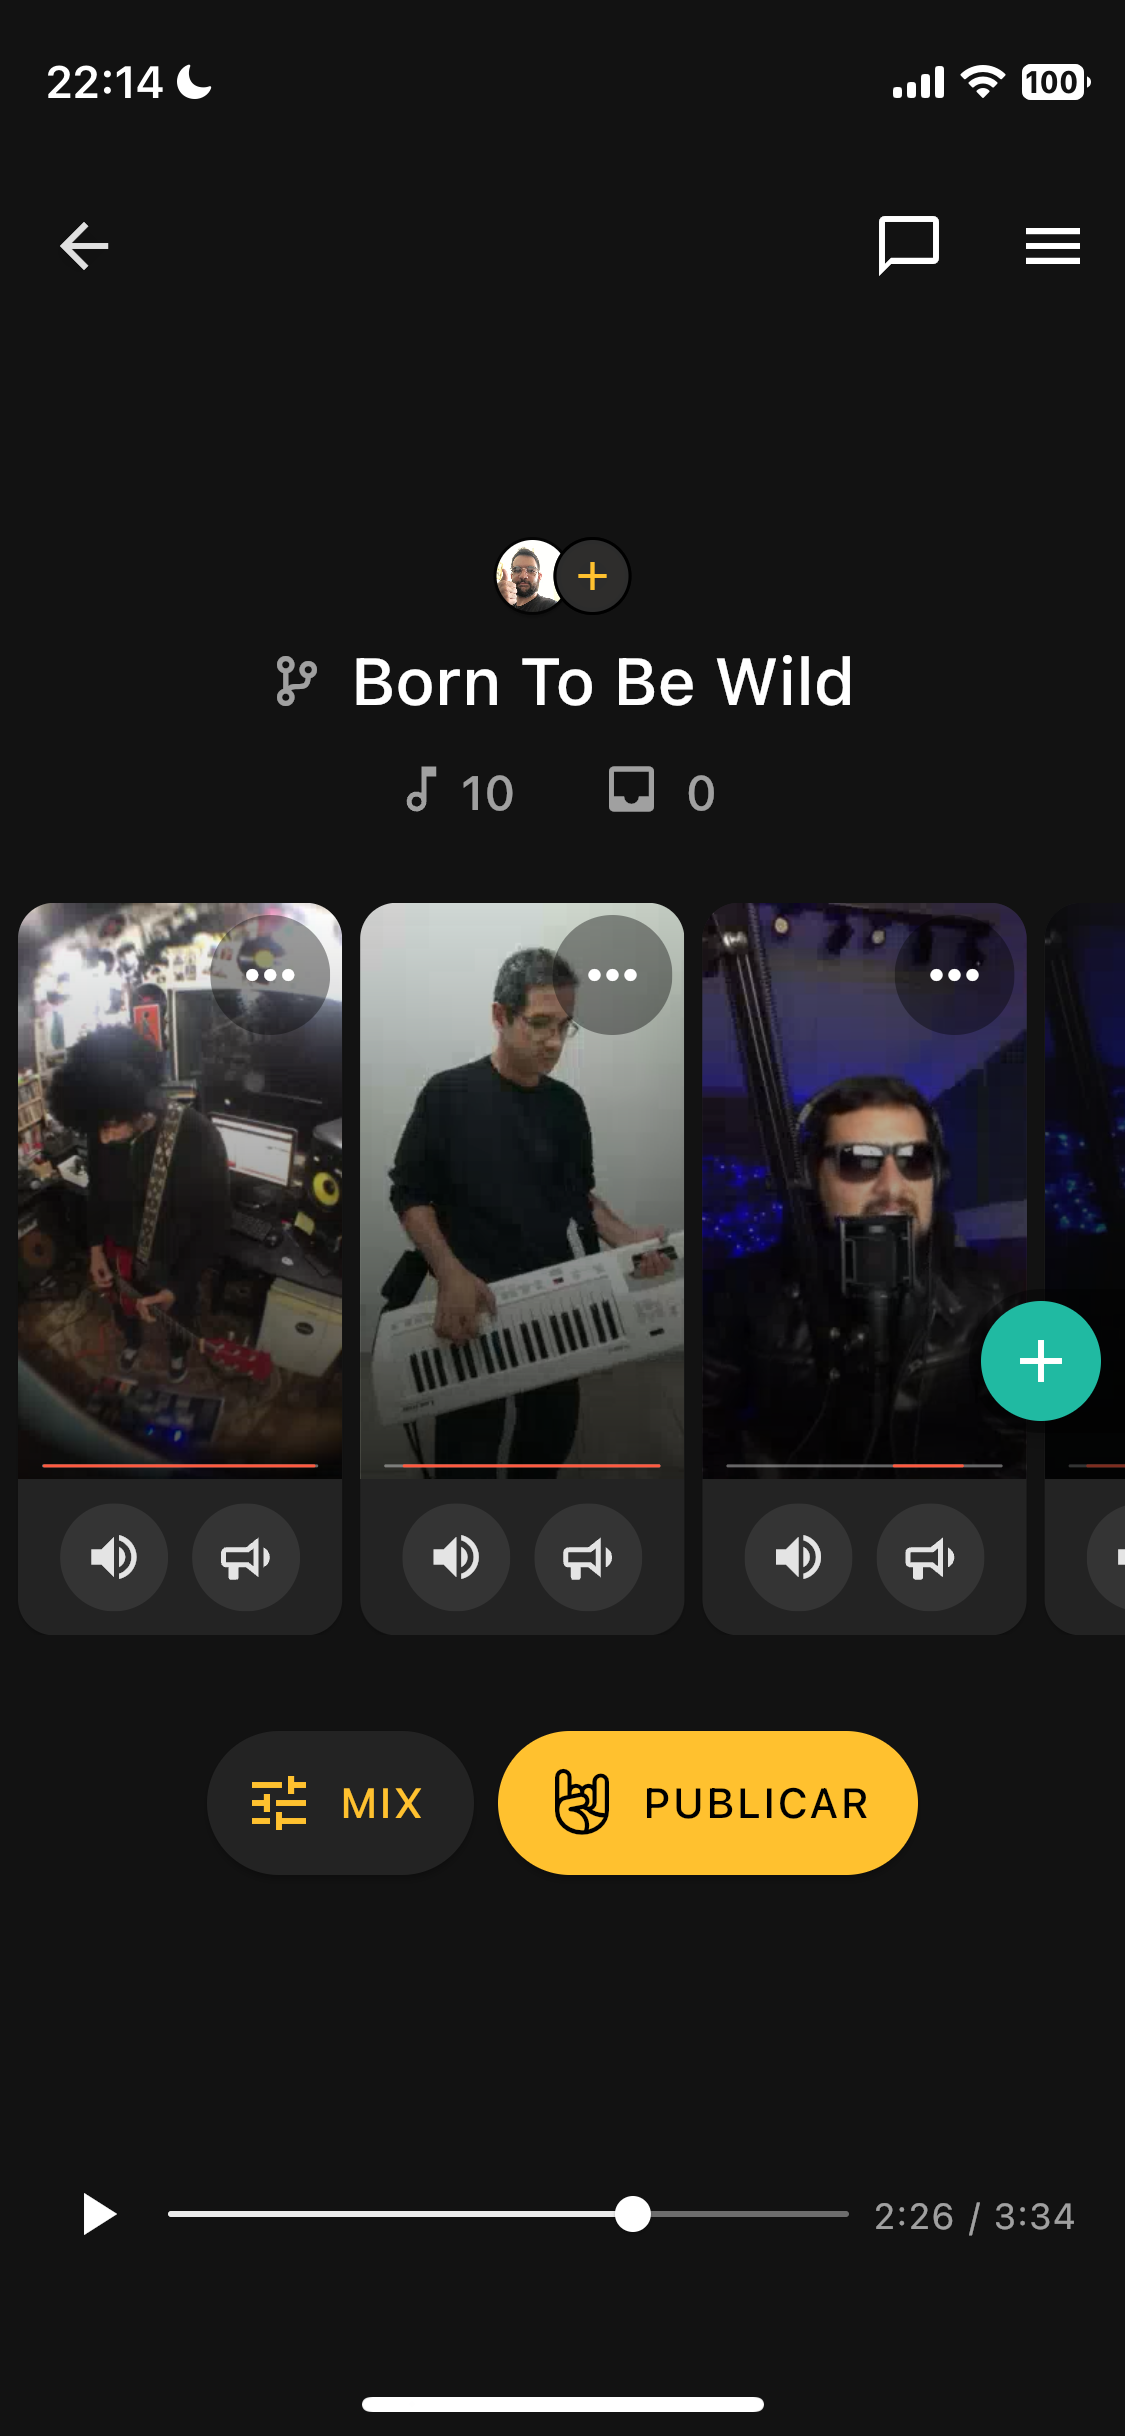
\includegraphics[width=0.24\textwidth]{chapters/chap01/images/inda/inda4.PNG}}
    \caption{Recursos do \textit{app Indaband}: (a) \textit{Home} (b) \textit{Feed} (c)
    \textit{Feed} (d) \textit{Studio}.}
    \label{fig:cap_tela}
\end{figure}

Indaband é uma aplicação móvel para distribuição e gravação de música
colaborativa e remota \cite{indaband}. A versão inicial foi disponibilizada
publicamente em Agosto de 2022. O quadro de funcionários é majoritariamente
brasileiro, enquanto que o produto possui distribuição global. A FIGURA
\ref{fig:cap_tela} exibe capturas de tela da interface visual.


O aplicativo móvel Indaband contém uma série de funcionalidades e abstrações
para a gravação e distribuição de música colaborativa. Para maior entendimento
do do sistema de recomendação a ser proposto, é necessário compreender as
principais entidades do aplicativo.


\subsubsection{Sessão}

Na aplicação, usuários podem criar sessões, que são ambientes colaborativos de
gravação entre os participantes. As sessões contam com ferramentas para gravação
e mixagem. O ambiente de pré-visualização, edição e produção da sessão chama-se
\textit{Studio}. Nesse ambiente, há funcionalidades de adição, edição,
remoção e mixagem de faixas. Sessão também é o nome dado ao conjunto de faixas
introduzidas pelos usuários que constituem uma determinada música.

A sessão contém uma funcionalidade de cabine de gravação, permitindo que os
participantes gravem faixas de áudio ou de vídeo. Além disso, o usuário pode
importar mídias de áudio ou de vídeo, tal que cada mídia importada equivale a
uma faixa.

O usuário que cria a sessão é considerado seu dono, enquanto os demais usuários
que aceitam o convite para ingressar são considerados participantes. Toda sessão
publicada é disponível para visualização pública e contém ao menos uma faixa. A
publicação pode ser posteriormente removida pelo dono da sessão.


\begin{figure}[h]
  \begin{center}
    \subfigure[]{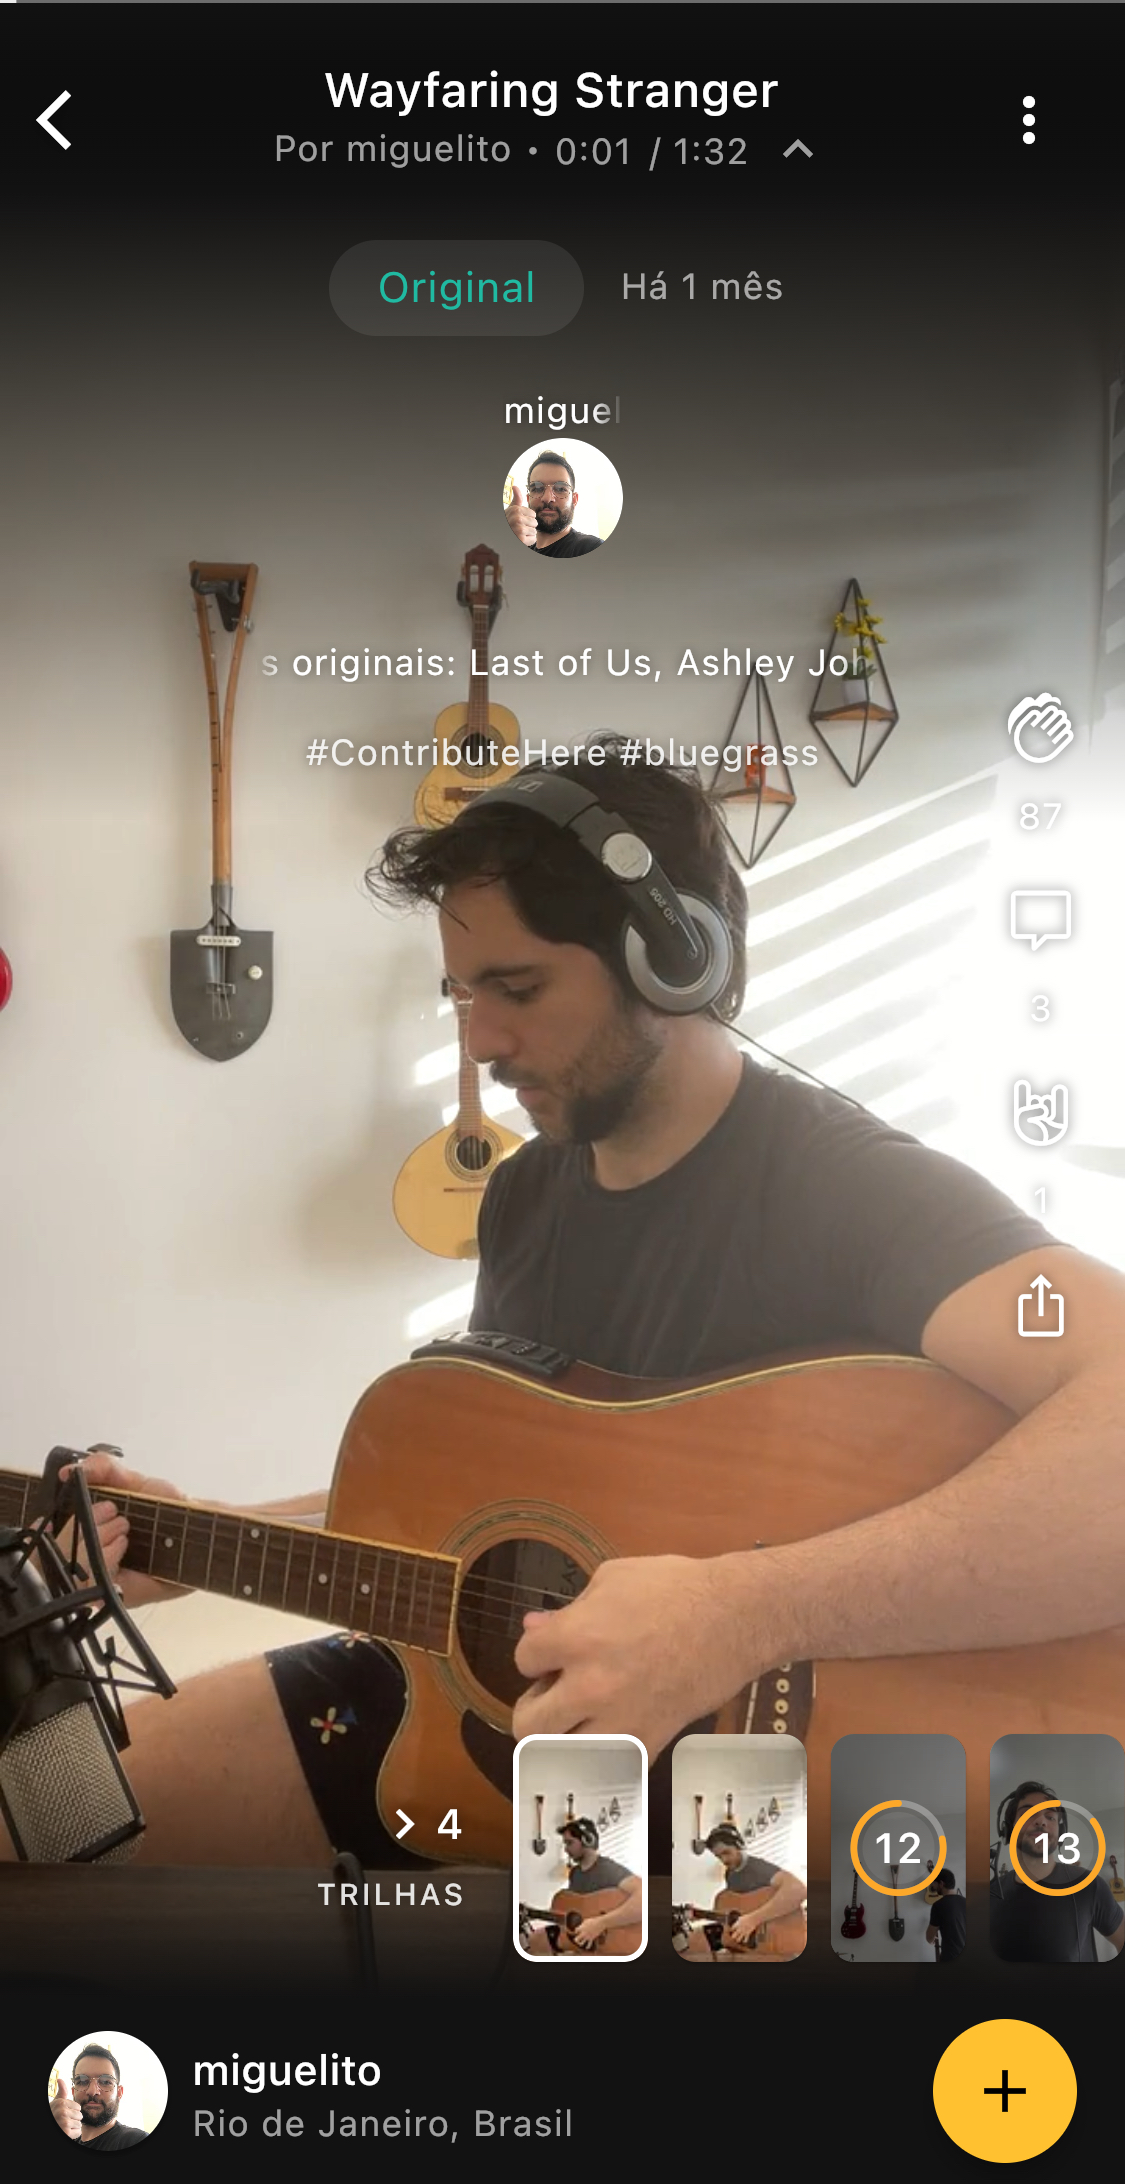
\includegraphics[width=0.4\textwidth]{chapters/chap02/images/wayfaring_original.jpeg}}
    \subfigure[]{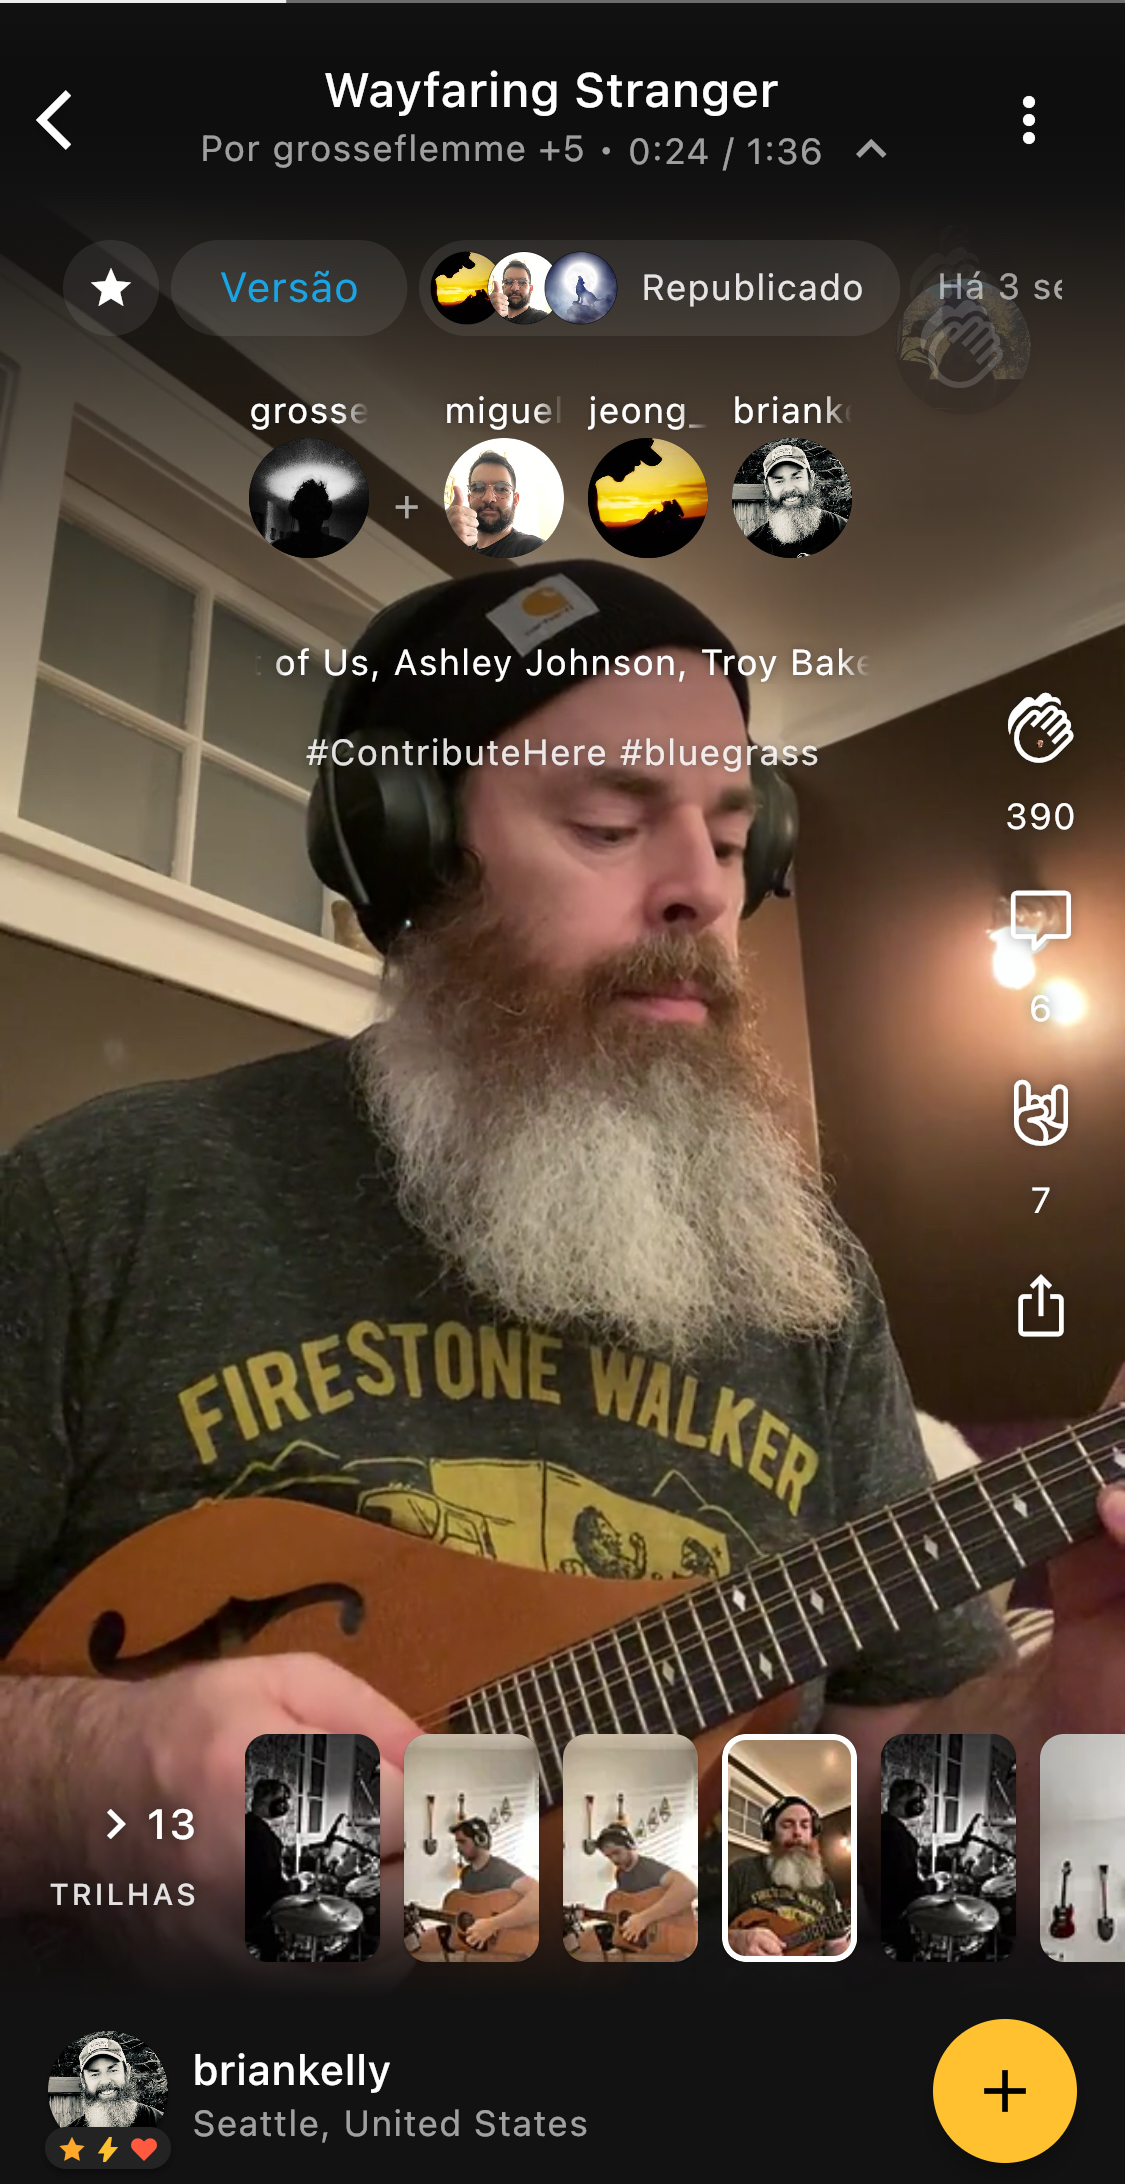
\includegraphics[width=0.4\textwidth]{chapters/chap02/images/wayfaring_fork.jpg}}
    \caption{Duas sessões publicadas no aplicativo Indaband. A primeira sessão é
    a sessão original, enquanto a segunda é um \textit{fork} subsequente da
    primeira. Ambas compartilham o mesmo nome e as faixas da primeira sessão. A
    segunda sessão contém faixas adicionais.}
    \label{fig:session_and_fork}
  \end{center}
  \end{figure}

\subsubsection{\textit{Fork}} Toda sessão publicada disponibiliza a
funcionalidade de \textit{fork} para os demais usuários da plataforma. O
\textit{fork} é uma cópia da sessão original, em que é possível adicionar
gravações inéditas, editar e remover faixas pré-existentes sem afetar a
publicação original. Quando publicada, a sessão \textit{fork} exibe o autor original das faixas
pré-existentes que forem mantidas, além da referência para a sessão anterior.

O \textit{fork} é uma das principais formas de colaboração assíncrona entre
usuários. A FIGURA \ref{fig:session_and_fork} ilustra duas sessões, sendo a
segunda um \textit{fork} subseqeuente da primeira. Note que a quantidade de
faixas e usuários presentes na segunda sessão aumenta. Além disso, conta com
maior quantidade de visualizações, comentários e outras formas de engajamento
positivo. Entre essas duas sessões, houve uma série de \textit{forks}
intermediários, realizados por cada um dos usuários que adicionaram faixas às
suas sessões.


\subsubsection{Faixa}
A faixa é uma mídia com áudio e vídeo que geralmente contém a gravação de um
instrumento ou voz. Uma faixa necessariamente é criada a partir de um entre três
recursos: tal como uma gravação original, tal como um \textit{fork} de uma faixa
publicada anteriormente ou como uma importação de uma mídia de áudio ou de
vídeo.




\section{Sobrecarga de informação}

Após três anos de desenvolvimento, a aplicação conta com dezenas de milhares de
usuários cadastrados, os quais centenas gravam mensalmente. Dado o grande
catálogo de usuários, o processo de encontrar pessoas com interesses musicais
similares demanda tempo e esforço. O mesmo ocorre ao procurar uma sessão que
seja de interesse em meio ao grande volume de conteúdo publicado. Essa
dificuldade percebida pelo usuário é conhecida na literatura de sistemas de
recomendação como sobrecarga de informação \cite{roetzel2019information}.

A sobrecarga de informação, segundo \citet{roetzel2019information}, é um estado em que um tomador de decisões observa um
conjunto ou uma carga de informações de complexidades distintas, a qual inibe a
capacidade do tomador de decisões de determinar de forma ótima a melhor decisão
possível.

\vspace{0.2cm}
\begin{figure}[h]
    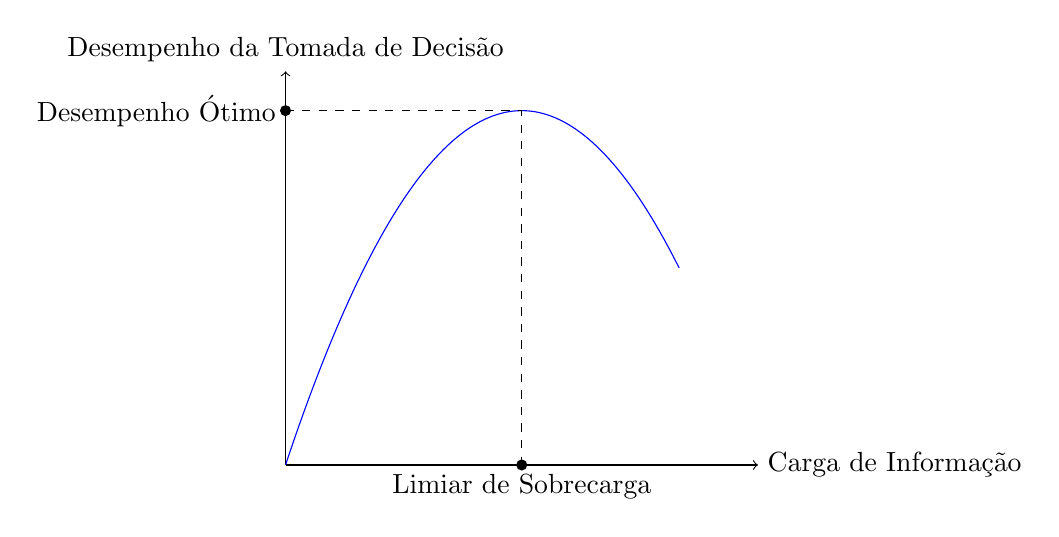
\begin{tikzpicture}
    % Eixo X
    \draw[->] (0,0) -- (6,0) node[right] {Carga de Informação};
    % Eixo Y
    \draw[->] (0,0) -- (0,5) node[above] {Desempenho da Tomada de Decisão};
  
    % Curva U invertida
    \draw[blue, domain=0:5, samples=100] plot (\x, {3*\x - 0.5*\x*\x});
  
    % Pontos de interesse
    \fill (0,4.5) circle (2pt) node[left] {Desempenho Ótimo};
    \fill (3,0) circle (2pt) node[below] {Limiar de Sobrecarga};

    % Linhas tracejadas
    \draw[dashed] (0,4.5) -- (3,4.5);
    \draw[dashed] (3,0) -- (3,4.5);
  \end{tikzpicture}
   % Descrição
    \caption{Correspondência entre a carga de informação e o desempenho da tomada
    de decisão.}
    \label{fig:u_invertida}
\end{figure}
\vspace{0.2cm}

O uso subótimo de informações é causado
pela limitação de recursos individuais escassos. Um recurso escasso pode ser uma
característica individual (como capacidade de processamento em série, memória de
curto prazo) ou equipamento relacionado à tarefa (por exemplo, orçamento ou
tempo para tomar uma decisão). A probabilidade de alcançar a melhor decisão
possível é definida como o desempenho de tomada de decisão. A correspondência
entre a carga de informação e o desempenho da tomada de decisão é ilustrada na
FIGURA \ref{fig:u_invertida} \cite{roetzel2019information}.

Experimentos realizados por \citet{liang2006personalized} mostraram que, ao
avaliar a satisfação de voluntários com um sistema de recomendação de notícias,
a precisão do conteúdo recomendado e o número de itens
recomendados influenciam diretamente na satisfação do usuário, reduzindo a
sobrecarga de informação e a insatisfação gerada pela sobrecarga.

\section{Sistemas de Recomendação}

\abbrev{RS}{sistemas de recomendação}
Sistemas de recomendação (RS, do inglês \textit{recommender systems}) são
ferramentas de \textit{software} que sugerem itens úteis para um usuário, de
acordo com a disponibilidade de seu histórico \cite{ricci2010introduction}. Esses
sistemas, que podem ser personalizados ou não-personalizados, ajudam usuários a
lidarem com processos de tomada de decisão em meio a sobrecarga de informações,
seja na escolha de um produto em um \textit{e-commerce} ou na seleção de um
filme em um serviço de \textit{streaming}. Ao contrário de uma ferramenta de
busca em que o usuário ativamente procura por um item específico, sistemas de
recomendação são úteis quando o usuário explora um catálogo diversificado,
otimizando a distribuição dos itens a partir de suas preferências pessoais. As
FIGURAS \ref{fig:spotify} e \ref{fig:twitter} ilustram sistemas de recomendação
para tarefas distintas: recomendação de \textit{playlists} na plataforma Spotify
e recomendação de perfis de usuário na plataforma Twitter, respectivamente.


\begin{figure}[ht]
    \centering
    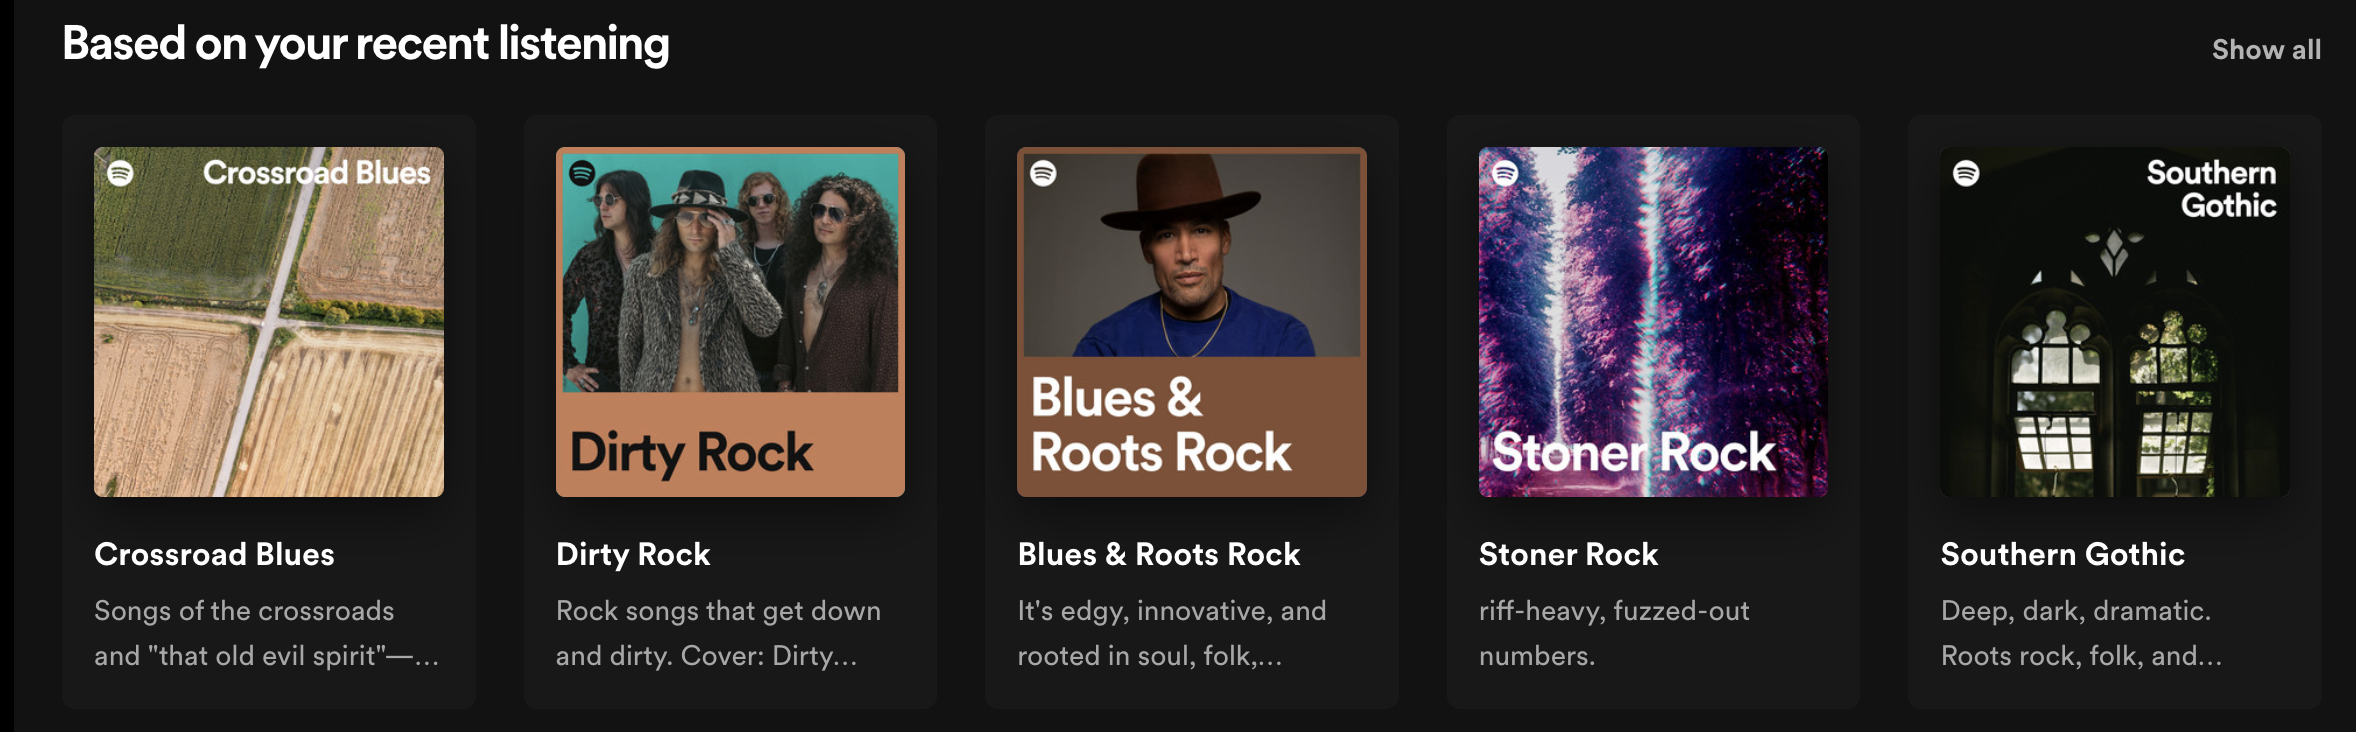
\includegraphics[width=0.8\textwidth]{chapters/chap01/images/spotify.png}
    \caption{Recomendações de \textit{playlists} no Spotify em Agosto de 2023.}
    \label{fig:spotify}
\end{figure}


Personalização é o processo de coleta e uso de informações pessoais para filtrar
conteúdo de forma única a um usuário, atendendo suas necessidades percebidas
pelo serviço ou declaradas explicitamente. \cite{liang2006personalized}.
Recomendações não-personalizadas distribuem o conteúdo recomendado de maneira
igualitária para todos os usuários, desconsiderando suas preferências
individuais. Uma recomendação a partir da lista de reportagens mais lidas em um
portal de notícias é um exemplo de recomendação não-personalizada.
\cite{falk2019practical}.

\begin{figure}[ht]
    \centering
    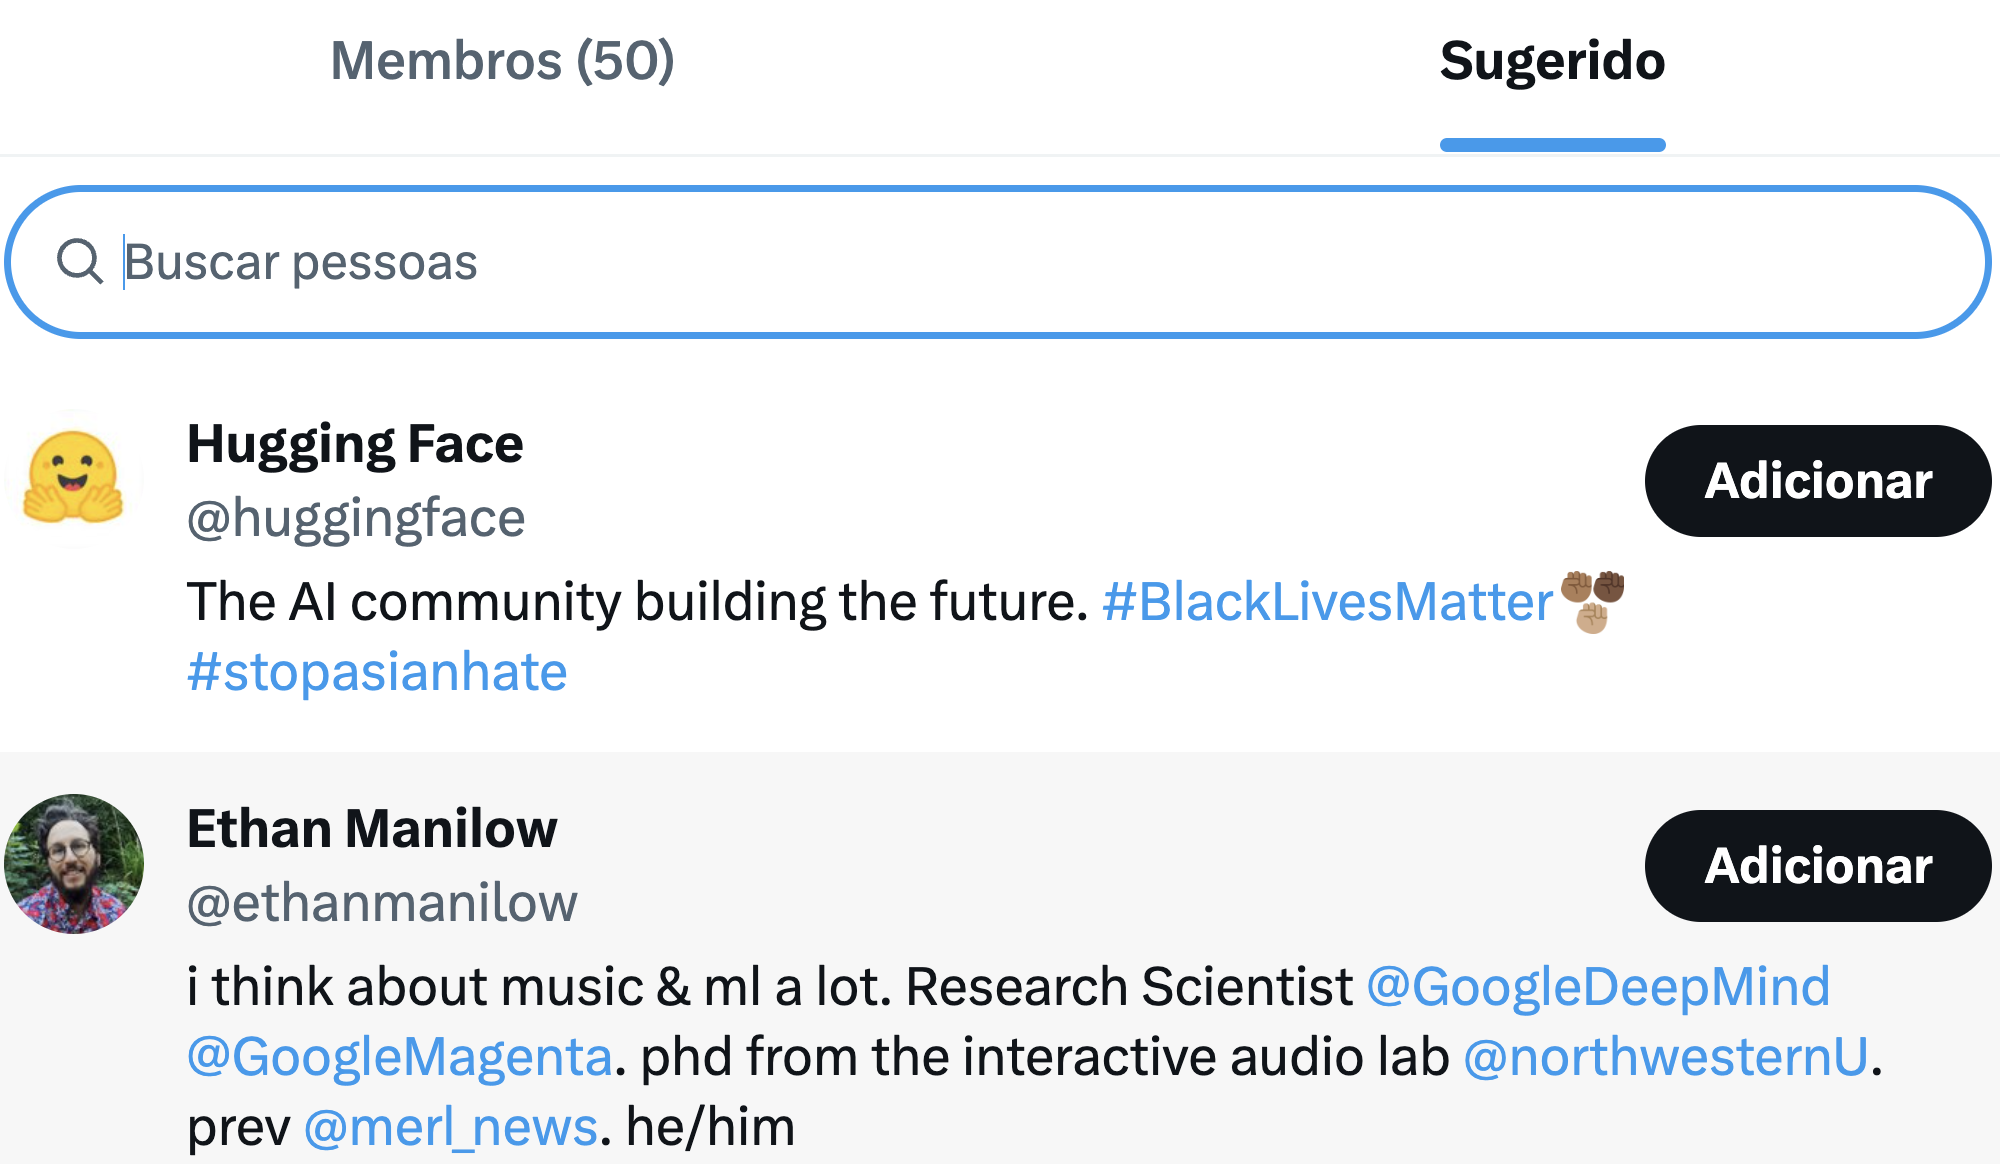
\includegraphics[width=0.6\textwidth]{chapters/chap01/images/tt.png}
    \caption{Recomendações de perfis de usuário no Twitter em Agosto de 2023.}
    \label{fig:twitter}
\end{figure}

% Sistemas de Recomendação Baseados em Sessão (SBRS, do inglês
% \textit{session-based recommender systems}) são sistemas de recomendação que 
Abordagens mais tradicionais em sistemas de recomendação modelam as interações
usuário-item na forma de uma matriz esparsa de avaliações. Cada linha da matriz
representa um usuário e cada coluna representa um item.

A tarefa em questão se
resume ao preenchimento dos valores faltantes da matriz, a depender da
abordagem escolhida. Valores preenchidos com avaliações altas são recomendados
ao usuário, uma vez que ele ainda não os consumiu, tal como ilustrado
na FIGURA \ref{fig:matriz_15}.


\begin{figure}[h]
    \centering
    \begin{tikzpicture}
        % Define the matrix
        \matrix (m) [matrix of nodes,
                    %  nodes in empty cells,
                     column sep=-\pgflinewidth,  % Adjust cell spacing
                     row sep=-\pgflinewidth,     % Adjust cell spacing
                     nodes={draw, text width=2.5em, align=center, minimum height=2.5em, minimum width=2.5em}] {
            5 & 4 & 1 & 1 \\
            4 & 4 & 1 & 1 \\
            1 & 2 &  & 4 \\
            1 & 1 & 4 & 4 \\
        };
      
        % % Labels on the left
        \foreach \row/\label in {1/Gilberto, 2/Maria, 3/Gal, 4/Caetano} {
          \node[left] at (m-\row-1.west) {\label};
        }
      
        % % Labels on the top
        \foreach \col/\label in {1/TV, 2/DVD, 3/sal, 4/pipoca} {
          \node[above,
          ] at (m-1-\col.north) {\label};
        }
      \end{tikzpicture}
      \caption{Matriz de avaliações para produtos de um comércio eletrônico. A predição atua sobre as avaliações não preenchidas.}
      \label{fig:matriz_15}
\end{figure}

\abbrev{SBRS}{Sistemas de recomendação baseados em sessão}
Por mais que a matriz de avaliações seja uma forma intuitiva de representação,
viabilizando uma boa variedade de modelos, trata-se de uma forma que
desconsidera o contexto temporal das interações ou a sequência específica de
itens que determinado usuário interagiu. Sistemas de Recomendação Baseados em
Sessão (SBRS, do inglês \textit{session-based recommender systems}) atuam
justamente nesse cenário.

Os SBRS se caracterizam pelos seus dados representarem um conjunto delimitado de
interações obtidas por \textit{feedback} implícito, ou seja, por preferências
indiretas identificadas a partir de ações ou padrões de navegação. Essas interações
são agrupadas em conjuntos denominados sessões. Uma sessão pode conter uma sequência temporalmente
ordenada de ações executadas por um usuário, ou um conjunto de ações executadas
por um usuário anônimo sem uma ordem específica.

Os objetivos de um SBRS incluem
prever a próxima interação do usuário durante uma sessão em andamento,
recomendar o próximo item ou um conjunto de itens para uma sessão, ou ainda
recomendar uma sessão inteira \cite{domingues_large_2023, survey_wang_2021}.


    



\begin{figure}[h]
    \centering
        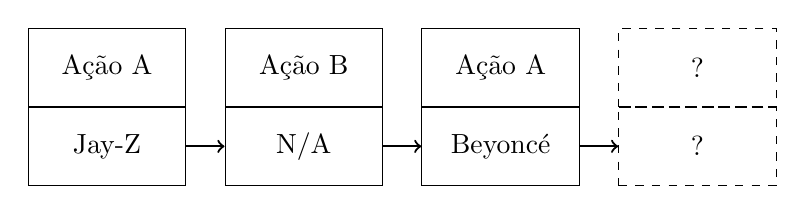
\begin{tikzpicture}
        % Draw the list cells
        \node[draw, rectangle, minimum width=2cm, minimum height=1cm] (cell1) at (0, 0) {Jay-Z};
        \node[draw, rectangle, minimum width=2cm, minimum height=1cm] (cell2) at (2.5, 0) {N/A};
        \node[draw, rectangle, minimum width=2cm, minimum height=1cm] (cell3) at (5, 0) {Beyoncé};
        \node[draw, dashed, rectangle, minimum width=2cm, minimum height=1cm] (cell4) at (7.5, 0) {?};

        % Draw the arrow
        \draw[->, thick] (cell1.east) -- (cell2.west);
        \draw[->, thick] (cell2.east) -- (cell3.west);
        \draw[->, thick] (cell3.east) -- (cell4.west);

        % % Add label to the left of the first cell
        % \node[left] at (cell1.west) {Sessão 1};

        % Draw the top cells with actions
        \node[draw, rectangle, minimum width=2cm, minimum height=1cm] (topcell1) at (0, 1.0) {Ação A};
        \node[draw, rectangle, minimum width=2cm, minimum height=1cm] (topcell2) at (2.5, 1.0) {Ação B};
        \node[draw, rectangle, minimum width=2cm, minimum height=1cm] (topcell3) at (5, 1.0) {Ação A};
        \node[draw, dashed, rectangle, minimum width=2cm, minimum height=1cm] (topcell4) at (7.5, 1.0) {?};

    \end{tikzpicture}
    \caption{Exemplo de uma sessão em andamento.}
    \label{fig:sessao_beyonce}
\end{figure}

Cada interação das sessões está associada a tuplas que contém um ou mais dos
seguintes dados: a ação executada, o item alvo da ação, o instante em que a ação
foi executada e o usuário responsável pela ação. Por exemplo, uma sessão pode
representar uma lista ordenada de itens selecionados por um usuário anônimo, ou
uma lista de ações executadas por usuários de uma mesma sessão, sem que essas
ações estejam necessariamente atreladas cada uma a um item. Isso é um aspecto
útil dos SBRS, por prover recomendações em aplicações em que não há distinção
entre usuários, ou quando as preferências de longo prazo de um usuário novo da
plataforma não foram identificadas. A FIGURA \ref{fig:sessao_beyonce} ilustra um
exemplo de sessão em andamento, em que a ação A corresponde a navegar ao perfil
de determinado artista, enquanto que a ação B corresponde a criar uma
\textit{playlist} vazia. Nem toda ação é necessariamente associada a um item,
como expresso na Ação B.
\vspace{0.4cm}
\section{Trabalhos Futuros}
% TODO: @Miguel - Needs review

A bibliografia existente de espectrograma de modulação, até o presente momento,
aplica uma segunda STFT sobre o domínio acústico, com a finalidade de medir
oscilações de intensidade no eixo da frequência. Dessa forma, o novo eixo obtido
pelo espectrograma de modulação representa modulações de amplitude.

Considerando
que o espectrograma acústico reside em um espaço vetorial $\mathbb{R}_3$, uma proposta de trabalho futuro é
investigar a possibilidade de representar modulações em frequência, bastando que a segunda
STFT meça as oscilações no eixo da frequência para uma dada intensidade
constante.
% \section{Modelagem com inclusão de instrumento e gênero}
\subsection{Base restrita a faixas inéditas} 

Uma característica particular das sessões do Indaband é a capacidade de criar
uma sessão a partir de outra já existente, modificá-la, adicionar novas
gravações e publicá-la como uma nova iteração a partir da funcionalidade de
\textit{fork}.

Essa funcionalidade é muito utilizada pelos usuários. A tabela \ref{tab_sessoes}
mostra que 76\% das faixas criadas são geradas via \textit{fork},
independentemente se foram publicadas ou não. Dessa forma, usuários distintos
podem contribuir para uma mesma sessão em momentos distintos, ou um usuário pode
contribuir para uma mesma sessão de outro usuário que era desconhecido até
então.

Uma vez que o objetivo é recomendar usuários prováveis de contribuir gravando
uma faixa inédita para uma determinada sessão, é razoável gerar um cenário em
que o recomendador seja treinado e avaliado estritamente para prever a próxima
faixa inédita gravada.

As abordagens \textit{next-item} e \textit{remaining-items} são as mais
utilizadas nos comparativos publicados porque aproveitam todos os itens de cada
sessão para o treinamento ou para a avaliação. No caso de uma aplicação em que
haja redundância entre as sessões, em que usuários possam salvar, repetir e
compartilhar sessões entre si, essas abordagens acabam por facilitar o trabalho
do recomendador, uma vez que cada iteração a mais no processo de treinamento
significa uma nova oportunidade para minimizar o erro do modelo. O mesmo vale
para a avaliação, em que identificar faixas \textit{forkadas} seria em tese uma
tarefa mais fácil. O cenário mais desafiador é aquele em que o item a ser
avaliado é necessariamente um item inédito no contexto daquela sessão.

Em contraponto, a abordagem \textit{last-item} é a que mais se aproxima do
cenário mencionado, uma vez que mantém inalterada a sequência de itens das
sessões. O que muda é a forma de avaliação, que passa a considerar apenas o
último item da sequência como o item a ser previsto, sem que os demais itens
anteriores sejam avaliados, minimizando a influência de itens \textit{forkados}
na avaliação.

Com essa finalidade, a base de treinamento do presente trabalho é filtrada:
Nesse último experimento, constam apenas sessões em que o último item da
sequência é a adição de uma faixa inédita. Essa identificação é feita a partir
de um metadado disponível, informando se a faixa foi gerada por um \textit{fork}
ou foi criada, seja por gravação, por importação de uma faixa ou por separação
de fontes.

Para essa abordagem, é utilizado o avaliador \textit{last-item}. Esse avaliador
considera apenas o último item da sequência como o item a ser previsto, sem que
os demais itens advindos de \textit{fork} sejam recomendados.

\begin{table}[htbp]
    \begin{tabular}{|l|l|l|l|l|l|l|l|}
      \hline
      Modelo & HR@5 & HR@10 & MRR@5 & MRR@10 & Cov@10 & Pop@10  \\
      \hline
      GNN & \textbf{0,551} & \textbf{0,625} & \textbf{0,437} & \textbf{0,446} & 0,660 & 0,202  \\
      \hline
      $\text{STAMP}_1$ & 0,519 & 0,584 & 0,377 & 0,386 & 0,610 & 0,217 \\
      \hline
      sknn2 & 0,518 & 0,647 & 0,213 & 0,230 & 0,643 & 0,169 \\
      \hline
      sknn1 & 0,515 & 0,642 & 0,209 & 0,226 & 0,592 & 0,197 \\
      \hline
      ct & 0,509 & 0,579 & 0,390 & 0,399  & 0,477 & 0,349 \\
      \hline
      $\text{STAMP}_2$ & 0,506 & 0,590 & 0,366 & 0,377 & 0,609 & 0,201 \\
      \hline
      $\text{NextItNet}_2$ & 0,465 & 0,563 & 0,341 & 0,354 & 0,566 & 0,249 \\
      \hline
      $\text{STAN}_2$ & 0,464 & 0,596 & 0,178 & 0,196 & 0,547 & 0,179 \\
      \hline
      $\text{STAN}_1$ & 0,451 & 0,572 & 0,186 & 0,202 & 0,529 & 0,177 \\
      \hline
      $\text{NextItNet}_1$ & 0,449 & 0,536 & 0,337 & 0,349 & 0,525 & 0,257\\
      \hline
      vsknn1 & 0,447 & 0,580 & 0,1193 & 0,211 & 0,544 & 0,208 \\
      \hline
      $\text{VSTAN}_1$ & 0,441 & 0,580 & 0,180 & 0,198 & 0,507 & 0,221 \\
      \hline
      $\text{SMF}_2$ & 0,439 & 0,553 & 0,291 & 0,306 & 0,306 & 0,240 \\
      \hline
      $\text{SMF}_1$ & 0,431 & 0,530 & 0,298 & 0,311 & 0,240 & 0,257 \\
      \hline
      vsknn2 & 0,427 & 0,564 & 0,172 & 0,190 & 0,618 & 0,163 \\
      \hline
      $\text{SR}_2$ & 0,423 & 0,534 & 0,277 & 0,291 & 0,471 & 0,238 \\
     \hline
      $\text{VSTAN}_2$ & 0,418 & 0,546 & 0,171 & 0,189 & 0,588 & 0,142 \\
      \hline
      $\text{SR}_1$ & 0,410 & 0,512 & 0,279 & 0,292 & 0,445 & 0,259 \\
      \hline
      ar & 0,395 & 0,498 & 0,248 & 0,262 & 0,454 & 0,265 \\
      \hline 
      $\text{NARM}_1$ & 0,361 & 0,455 & 0,229 & 0,241 & 0,658 & 0,199 \\
      \hline
      $\text{NARM}_2$ & 0,324 & 0,440 & 0,211 & 0,226 & 0,665 & 0,188 \\
      \hline
      FOSSIL & 0,287 & 0,420 & 0,137 & 0,154 & 0,776 & 0,249 \\
      \hline
      FPMC & 0,281 & 0,419 & 0,124 & 0,143 & 0,764 & 0,241 \\
      \hline
      FISM & 0,275 & 0,434 & 0,120 & 0,141 & 0,749 & 0,240 \\
      \hline
      BPRMF & 0,271 & 0,407 & 0,122 & 0,141 & 0,744 & 0,250 \\
      \hline
      CSRM & 0,264 & 0,343 & 0,158 & 0,168 & 0,596 & 0,137  \\ 
      \hline
      $\text{GRU4Rec}_2$ & 0,208 & 0,278 & 0,130 & 0,139 & 0,873 & \textbf{0,030}  \\
      \hline
      $\text{GRU4Rec}_1$ & 0,195 & 0,271 & 0,123 & 0,134 & \textbf{0,858} & 0,040  \\
      \hline
      rpop & 0,165 & 0,225 & 0,106 & 0,113 & 0,009 & 0,319 \\
      \hline
      pop & 0,127 & 0,242 & 0,083 & 0,098 & 0,006 & 0,530 \\
      \hline
      spop & 0,125 & 0,219 & 0,059 & 0,071 & 0,299 & 0,471 \\
      \hline
      random & 0,003 & 0,005 & 0,001 & 0,001 & 1,000 & 0,014 \\
      \hline
      \end{tabular}
      \label{tab:results_last_item_final}
    \caption{Resultado dos modelos \textit{session-based} na abordagem
    \textit{single item}, avaliando o último item da sessão. Modelos ordenados por HR@5. }
  \end{table}

  A tabela \ref{tab:results_last_item_final} mostra os resultados obtidos pela
  abordagem \textit{last-item}. As métricas obtiveram valores na mesma faixa da
  abordagem \textit{next-item}, demonstrando que, por mais que a avaliação e o
  treinamento seja reservados apenas ao último item da sequência, os modelos
  mantém desempenho equivalente.
  
  Novamente, o modelo GNN obteve os melhores resultados. Modelos
  mais simples, como o skNN e a árvore de contexto também obtiveram bons
  resultados.





\section{Filtragem de Modulação} \label{section_fil_mod}
A filtragem de modulação é uma técnica para filtragem de envoltórias com
oscilações lentas, presentes em sub-bandas de frequência, aplicada sobre sinais
não-estacionários.\cite{clark2009sum} \cite{li2005properties}. O objetivo, em
aplicações de fala, é obter um sinal mais inteligível na saída, composto apenas
pela composição de tons com modulações de baixa frequência associadas à
articulação vocal, eliminando as demais parcelas.

Essa técnica assume que um sinal $x[n]$ de valores reais é
representado pela soma dos produtos entre moduladora e portadora que compõem
cada sub-banda $x_k[n]$:
\begin{equation}
    x[n] = \sum_{k = 0}^{K - 1} x_k[n] = \sum_{k = 0}^{K - 1} m_k[n] c_k[n]
\end{equation}


A implementação genérica da filtragem de modulação está representada no diagrama de blocos abaixo.

\begin{figure}[h]
    \centering
    \begin{tikzpicture}[auto,>=latex']
        \tikzstyle{block} = [draw, shape=rectangle, minimum height=3em, minimum
        width=3em, node distance=4cm, line width=1pt]
        %Creating Blocks and Connection Nodes
        \node at (-2.5,0) (input) {$x[n]$};
        \node [block] (filterbank) {Banco de filtros};
        \node [block, right of=filterbank] (dem) {demodulação};
        \node [block, right of=dem] (LP) {passa-baixas};
        \node [block, below of = filterbank] (sintese) {síntese};
        \node [block, below of=dem] (res) {reconstrução};
        \node [left of=sintese, node distance=2.5cm] (output) {$x'[n]$};
        %Conecting Blocks
        \begin{scope}[line width=1pt]
            \draw[->] (input) -- (filterbank);
            \draw[->, line width=1mm] (filterbank) -- node[name=subband] {$x_k[n]$} (dem);
            \draw[->, line width=1mm] (dem) -- node[name=mod] {$m_k[n]$} (LP);
            \draw[->, line width=1mm] (dem) -- node[name=carrier] {$c_k[n]$} (res);
            \draw[->, line width=1mm] (LP) |- node[name=new_mod] {$m'_k[n]$} (res);
            \draw[->, line width=1mm] (res) -- node[name=new_subband] {$x'_k[n]$} (sintese);
            \draw[->] (sintese) -- (output);
        \end{scope}
    \end{tikzpicture}
    \caption{Filtro de modulação, em diagrama de blocos. Adaptado de \cite{li2005properties}.}
\end{figure}

O sinal banda-larga $x[n]$ passa por um banco de filtros, no qual as  $x_k[n]$
saídas do banco de filtros passam por um módulo de demodulação, no qual são
separadas as parcelas moduladoras $m_k[n]$ e portadoras $c_k[n]$ de cada
sub-banda. Cada parcela $m_k[n]$ é filtrada por um filtro passa-baixas, cuja
resposta ao impulso é $g[n]$. Em seguida, cada sub-banda é reconstruída a partir da portadora
$c_k[n]$ e da modulação filtrada $m'_k[n]$. Finalmente, o sinal de banda larga
$x'_k[n]$ é sintetizado com as sub-bandas $x'_k[n]$ reconstruídas, obtidas a
partir das modulações filtradas.

Em aplicações de \textit{Speech Enhancement}, o projeto do banco de filtros
emula a resposta em frequência da cóclea no sistema auditivo. Por sua vez, a
frequência de corte do filtro passa-baixas é tipicamente de 16Hz
\cite{drullman1994}, tal que frequências abaixo desse valor estão associadas às
periodicidades na construção de frases, palavras e sílabas.

Uma forma de calcular $m'_k[n]$ é a partir do espectro de modulação $P_k[\mu]$,
apresentado na equação \ref{modspec_filterbank}:

\begin{equation}
    m'_k[n] = g[n] \ast m_k[n] = \sum_{q = 0}^{n} g[n - q] m_k[q]
\end{equation}

\begin{equation}
    m'_k[n] = \sum_{\mu=0}^{N-1} G[\mu]P_k[\mu] e^{j \frac{2 \pi \mu}{N} n}
\end{equation}  \todo{janela na eq?}

Dessa forma, obtém-se $m'_k[n]$ a partir da transformada inversa do espectro de
modulação filtrado por $G[\mu]$ \cite{toolbox2010}.

\todo{specs de implementação}
  %%________________________

   %%________________________
  %% CHAPTER 04
  \chapter{\textit{Speech Enhancement} Aplicado a \textit{Beamformers}}
\section{Indaband}
A música, enquanto atividade e produto, permite o estabelecimento de laços sociais
entre musicistas e ouvintes.

A atividade musical permite que um conjunto de musicistas interaja e
comunique-se, facilitada quando os membros compartilham de uma mesma bagagem
cultural. Além disso, permite que a audiência estabeleça um vínculo com
o músico executor ou o conjunto de musicistas \cite{cook2021music}.

Por sua vez, a música enquanto produto permite o estabelecimento de laços sociais
entre os ouvintes, seja em uma sala de concerto no século XIX, em uma sala de estar
com um rádio ou um gramofone no século XX, ou em uma apresentação ao vivo na
plataforma Twitch no século XXI.

Durante a pandemia de COVID-19, estudantes de música precisaram adaptar seus
hábitos de prática musical para aulas remotas e práticas individuais. A prática
coletiva foi fortemente afetada, uma vez que as aulas e os ensaios presenciais
foram suspensos em uma série de instituições de ensino, dado o risco de
contaminação e a necessidade de distanciamento social \cite{nusseck2021musical}.

A prática remota síncrona, hoje, enfrenta uma série de desafios técnicos. A
latência entre os praticantes é o principal problema. O limiar da percepção
auditiva para atrasos é de cerca de 20 milissegundos, enquanto que sistemas VoIP
com latência de 150 milissegundos e \textit{jitter} de 30 milissegundos são
considerados de boa qualidade. A codificação associada à compressão do sinal e a
largura de banda também influenciam no atraso. Enquanto a latência em uma
comunicação instantânea não for inferior ao limiar da percepção, essa forma de
prática musical não será viável.

A principal alternativa é a prática musical colaborativa assíncrona. Nesse
cenário, cada praticante grava sua faixa de forma individual enquanto ouve as
demais faixas gravadas. Aplicações como \textit{BandLab}, \textit{Ableton Live}
e \textit{Soundtrap by Spotify} funcionam sob essa abordagem.

Uma segunda característica da prática musical coletiva, seja no contexto
presencial ou remoto, é a necessidade de encontrar outros interessados com
gostos musicais similares, instrumentos que se complementem, etc. Uma pessoa que
deseja tocar um estilo musical específico, incomum na região em que vive,
sofreria dessa dificuldade. Um meio de resolver esse problema é recorrer à
comunidades virtuais ou redes sociais. Ao encontrar outros interessados, caso a
distância impeça a prática presencial, a atividade pode ser realizada a partir
da prática musical colaborativa assíncrona. Plataformas como \textit{Cifra Club}
e \textit{Ultimate Guitar} permitem que usuários contribuam com tablaturas de
músicas e comentários, formando uma comunidade virtual.


Tanto a prática musical colaborativa assíncrona quanto a formação de comunidades
virtuais de música são problemas os quais o mercado oferece poucas soluções
integradas. Estações de trabalho de áudio digital (DAWs, do inglês
\textit{Digital Audio Workstations}) mais tradicionais, como \textit{Pro Tools},
\textit{Logic Pro} e \textit{Ableton Live} são desprovidos de funcionalidades de
interação social. \textit{Cifra Club} e \textit{Ultimate Guitar} não permitem a
gravação colaborativa de forma assíncrona. \textit{Soundtrap by Spotify} e
\textit{BandLab} permitem a edição colaborativa em tempo real, porém apenas o
último contém funcionalidades de interação e integração social entre usuários. A
aplicação \textit{Collab}, da Meta, preenchia parcialmente esses critérios antes
de ser descontinuada. O aplicativo móvel Indaband foi criado para ocupar esse
espaço pouco preenchido no mercado.

\begin{figure}[h]
    \centering
    \subfigure[]{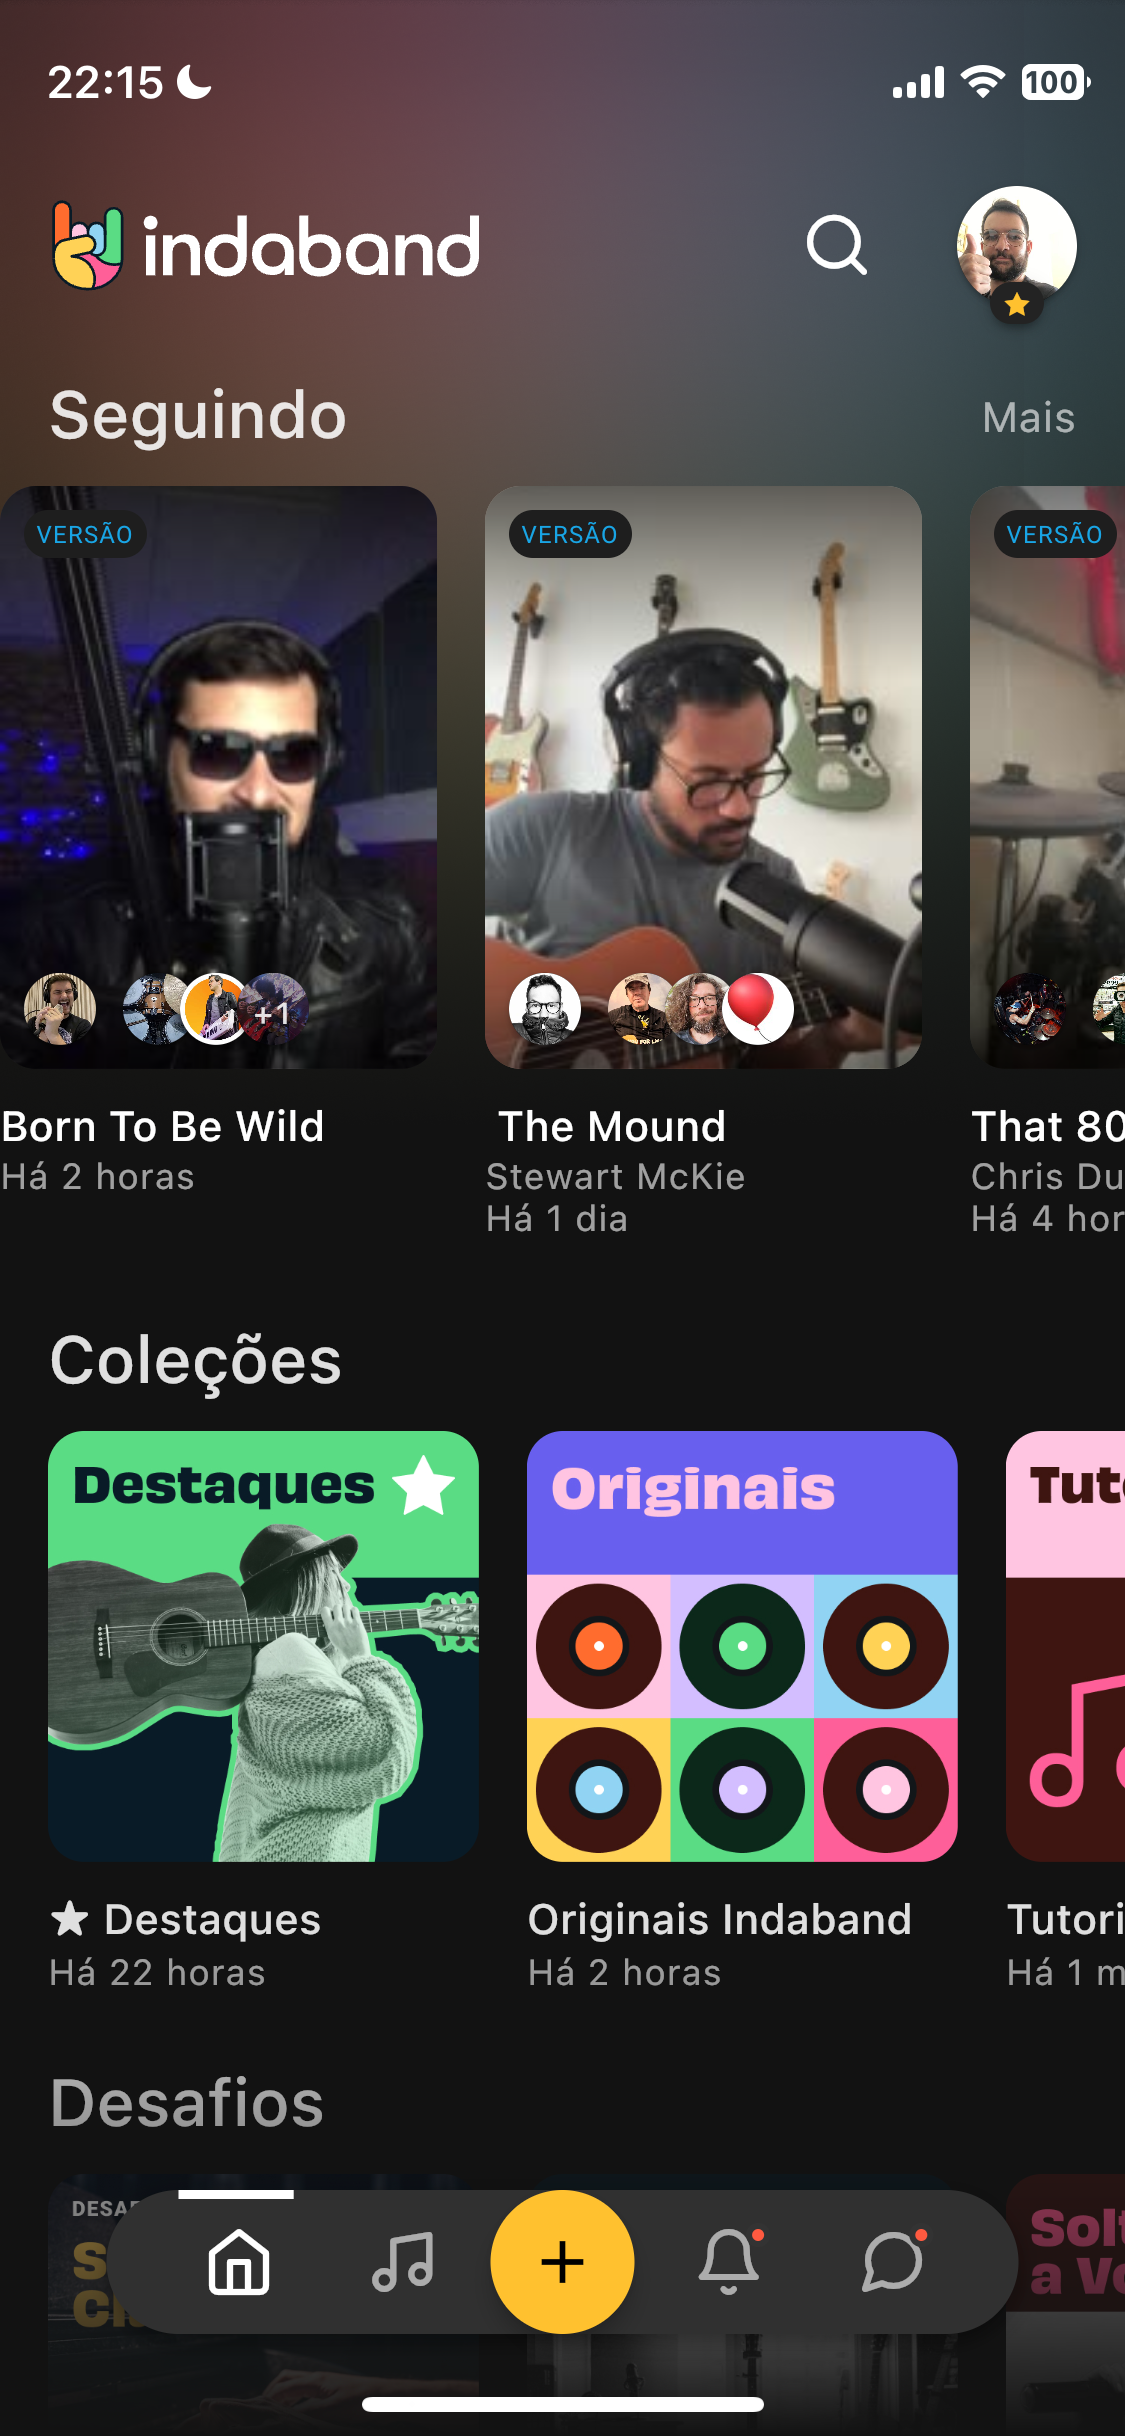
\includegraphics[width=0.24\textwidth]{chapters/chap01/images/inda/inda3.PNG}}
    \subfigure[]{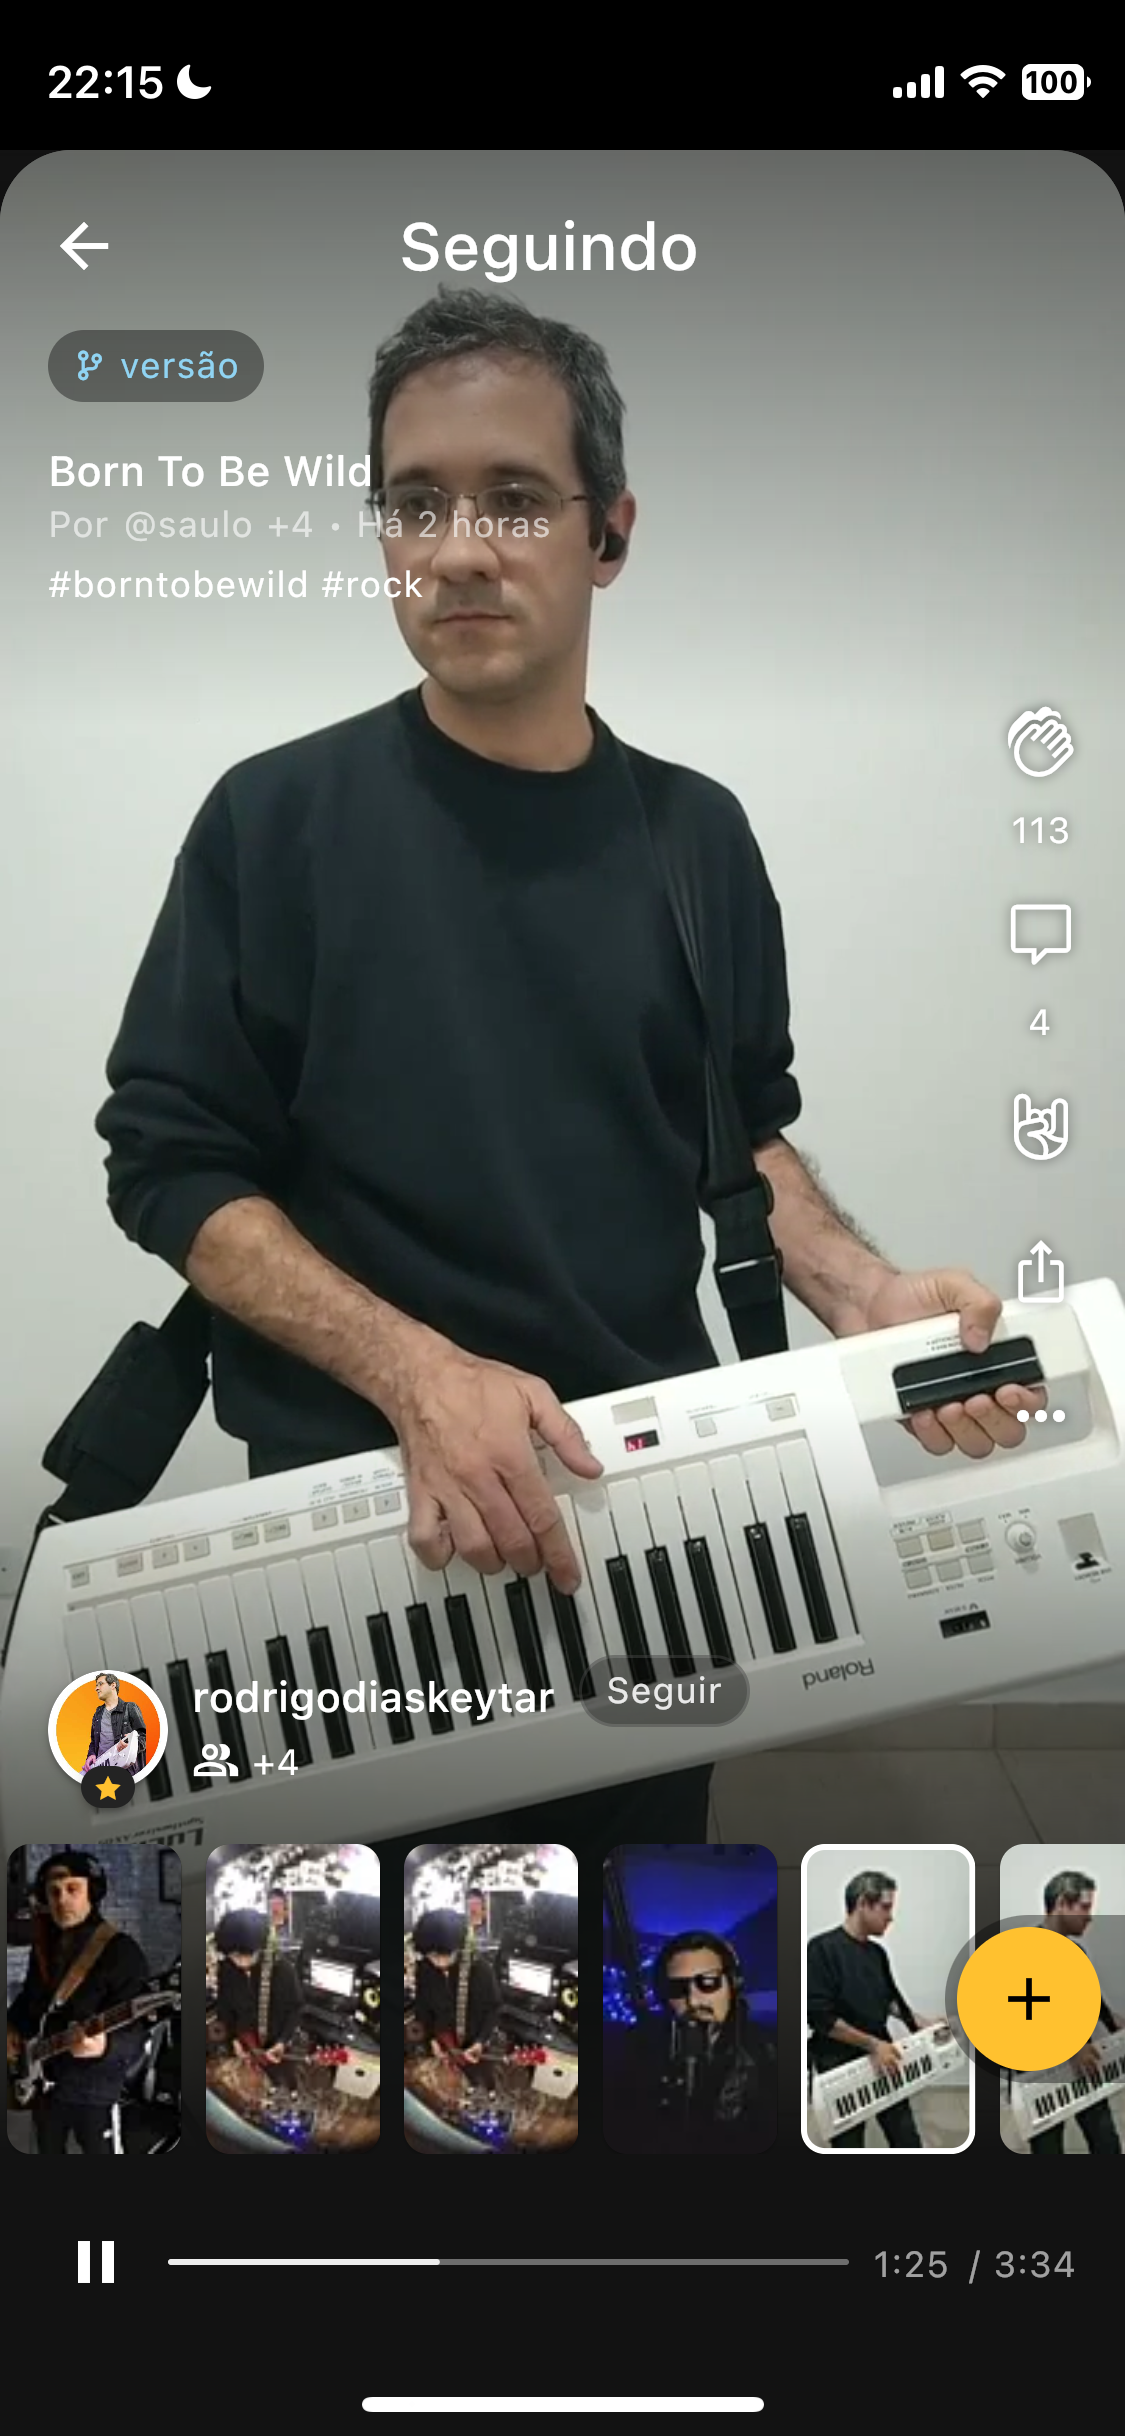
\includegraphics[width=0.24\textwidth]{chapters/chap01/images/inda/inda.PNG}}
    \subfigure[]{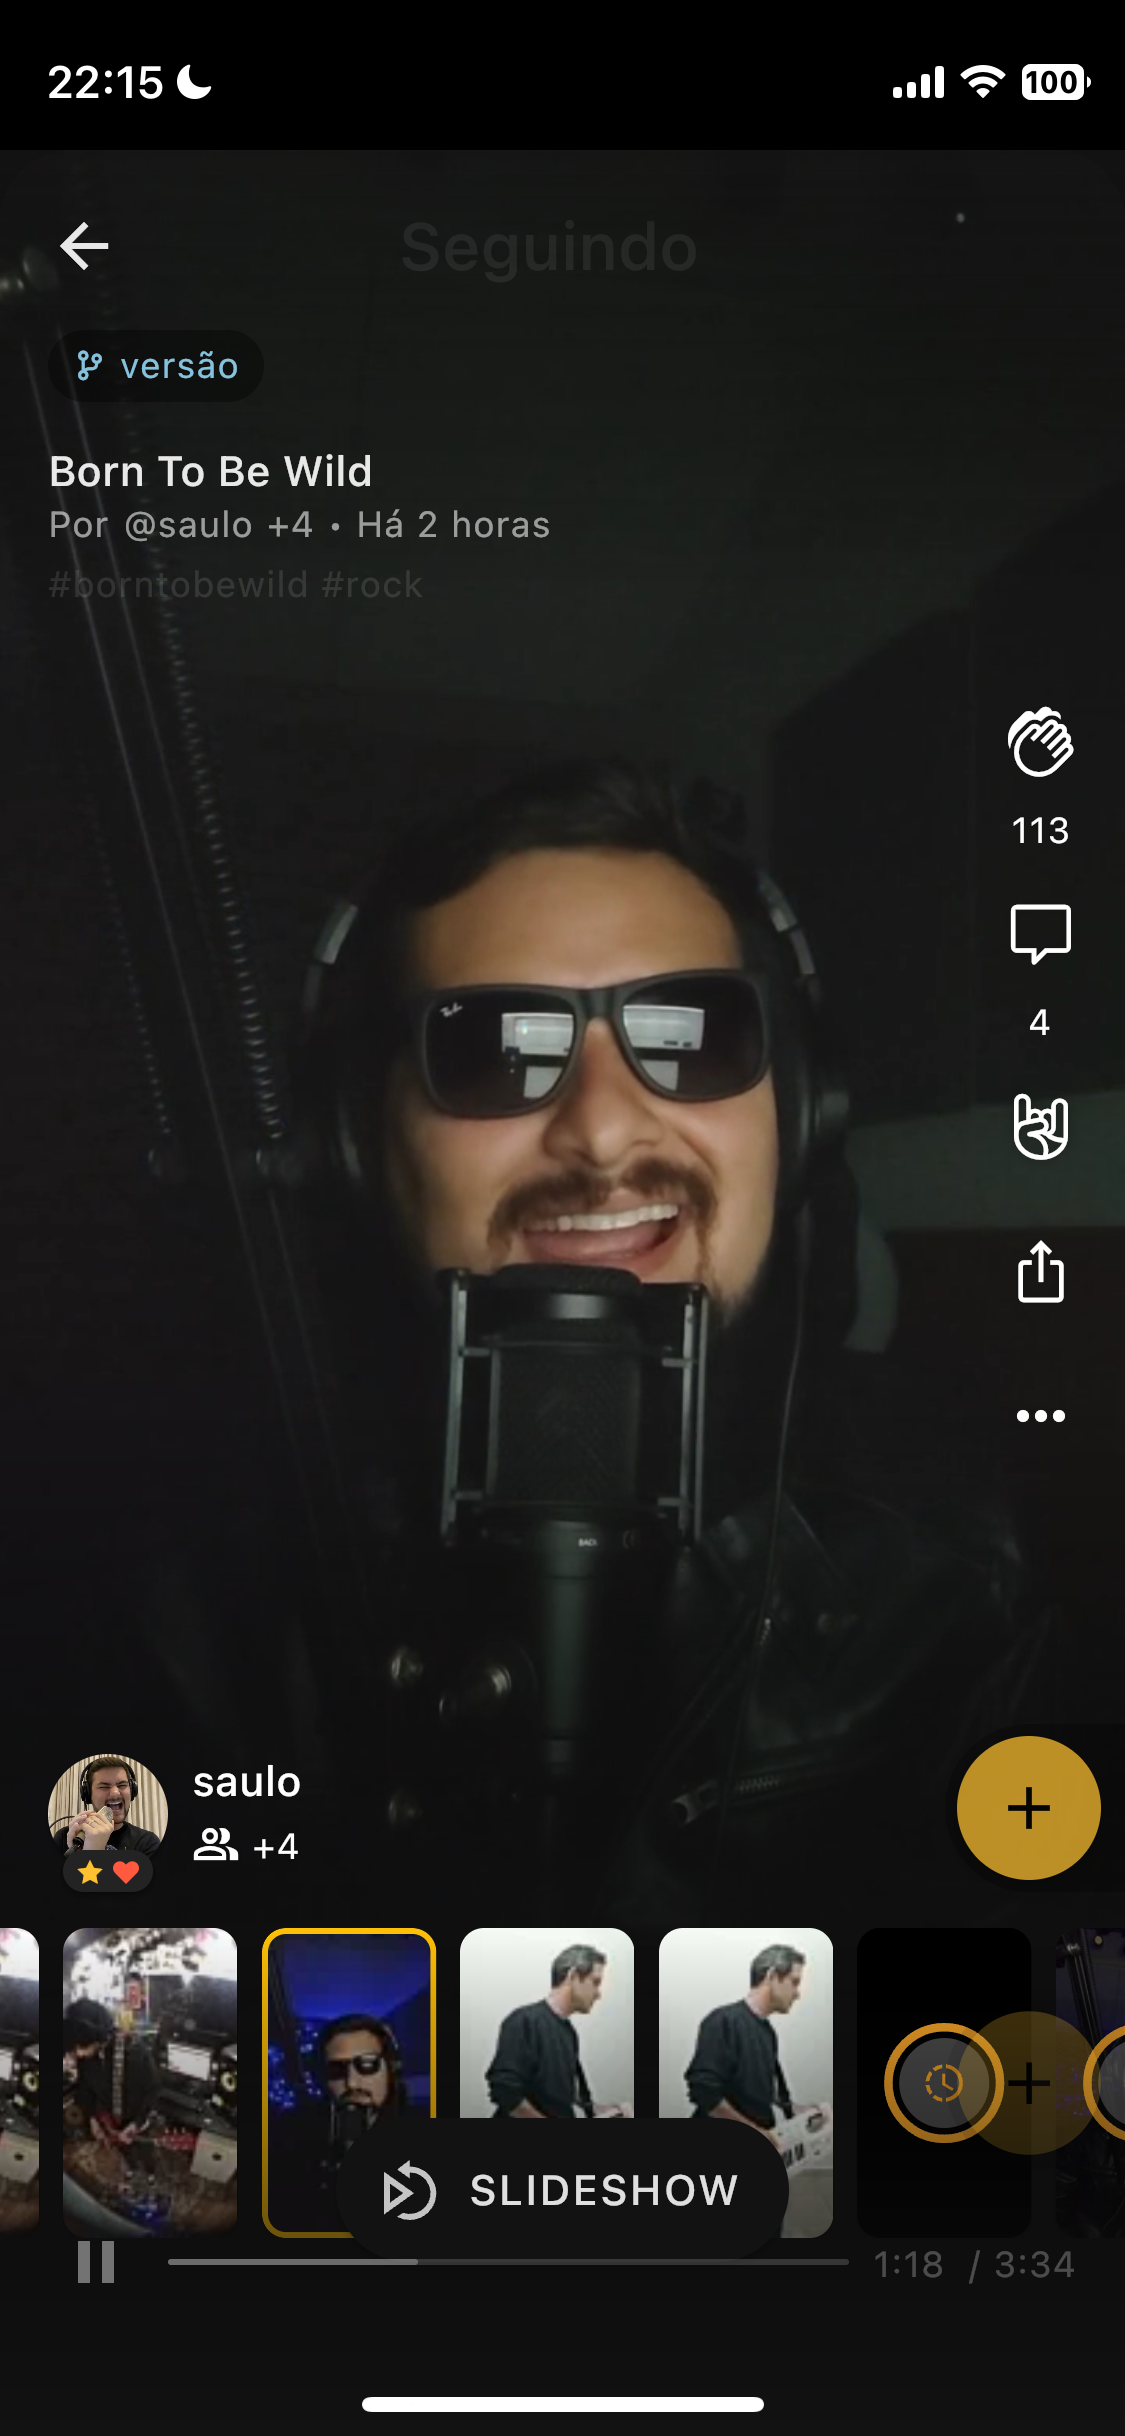
\includegraphics[width=0.24\textwidth]{chapters/chap01/images/inda/inda2.PNG}}
    \subfigure[]{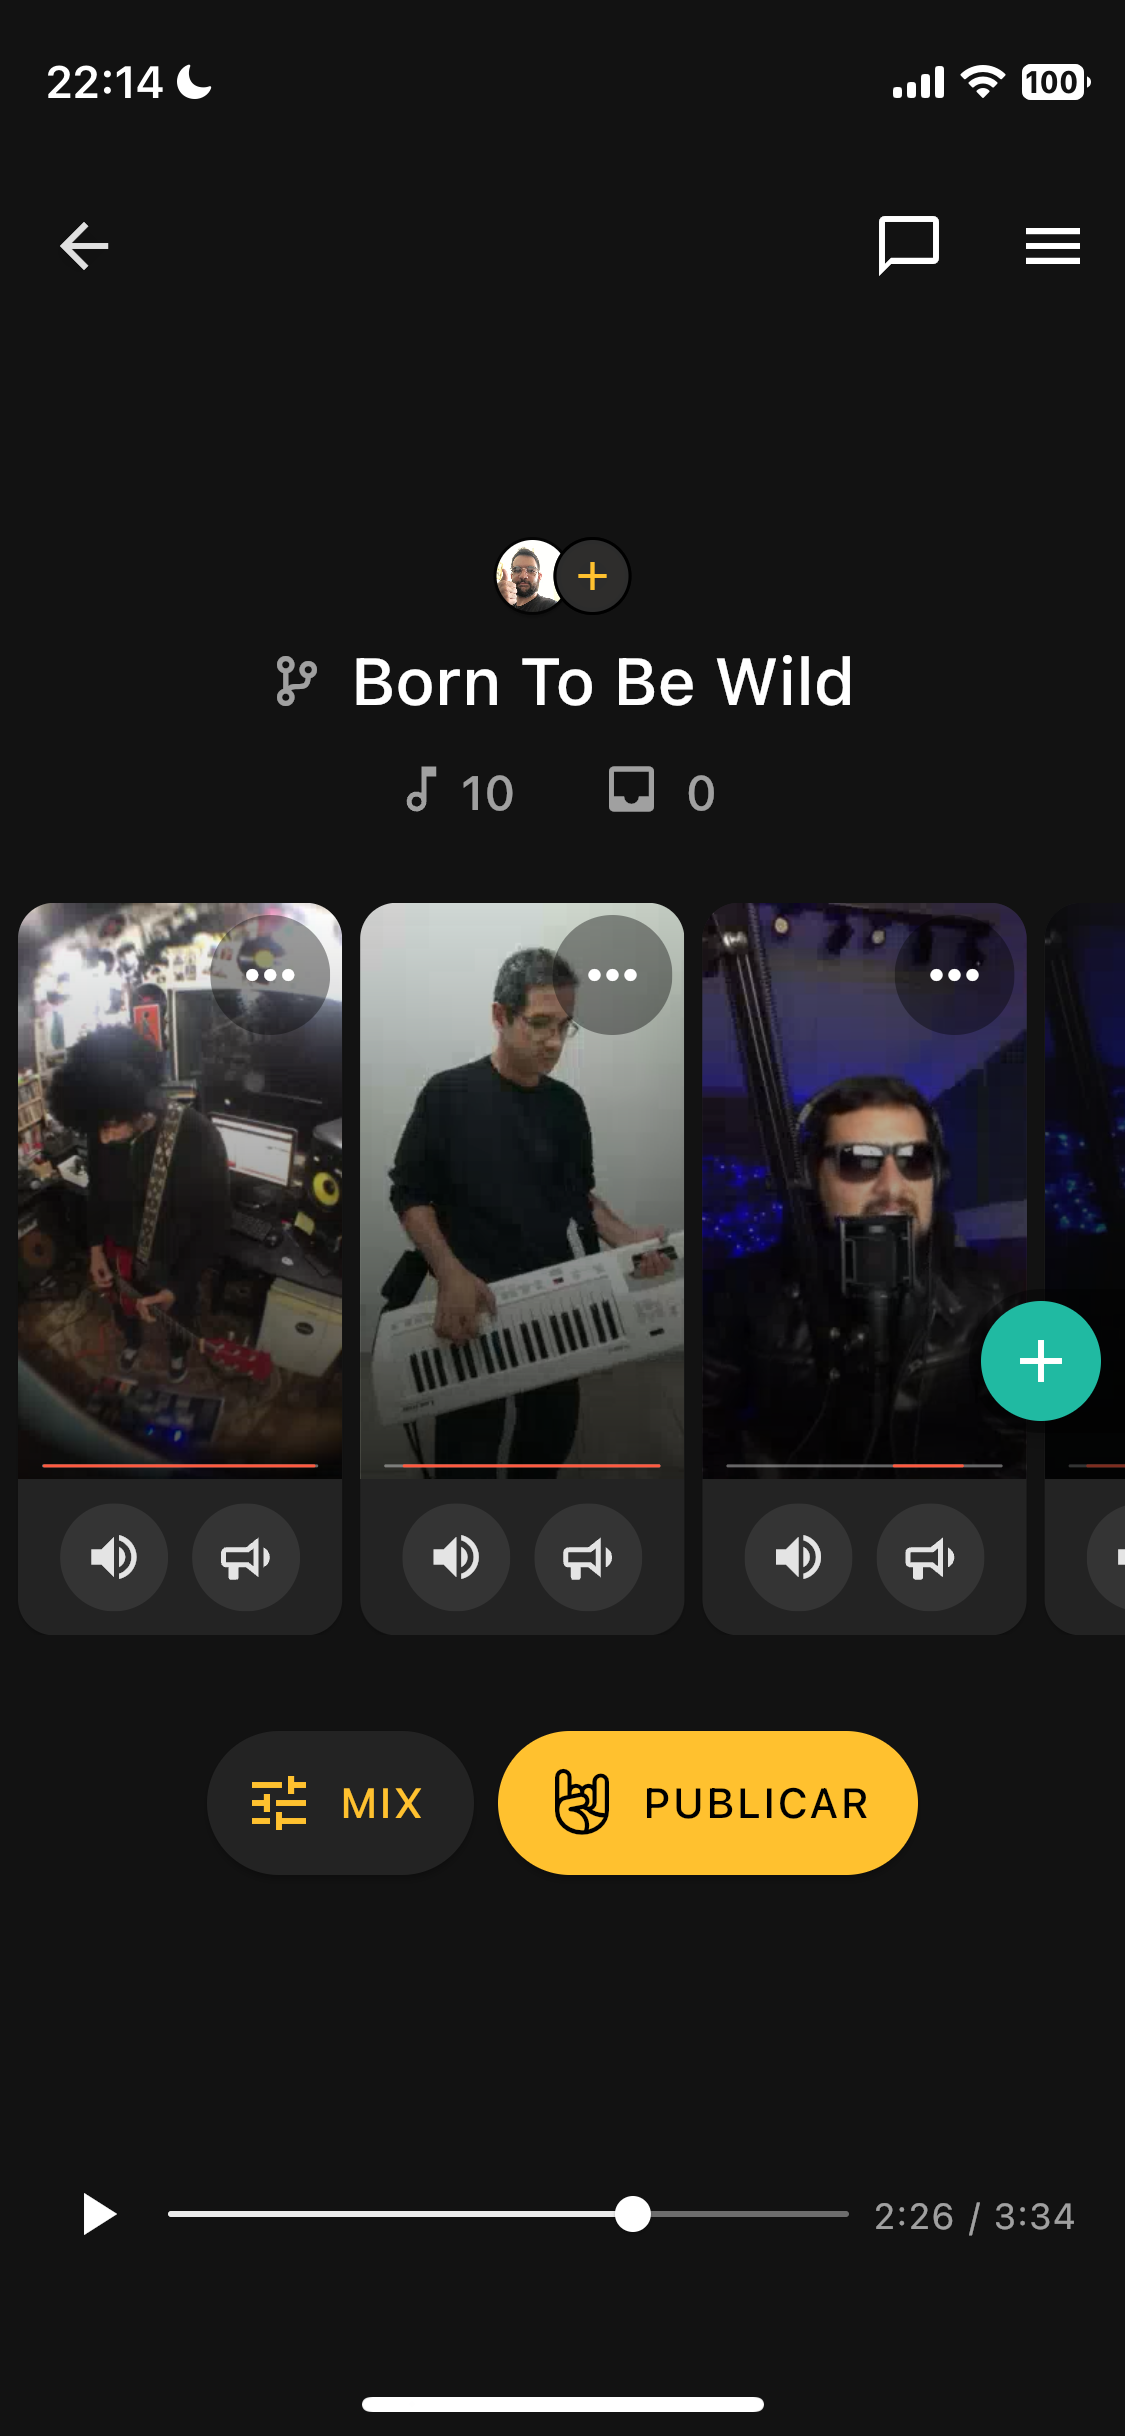
\includegraphics[width=0.24\textwidth]{chapters/chap01/images/inda/inda4.PNG}}
    \caption{Recursos do \textit{app Indaband}: (a) \textit{Home} (b) \textit{Feed} (c)
    \textit{Feed} (d) \textit{Studio}.}
    \label{fig:cap_tela}
\end{figure}

Indaband é uma aplicação móvel para distribuição e gravação de música
colaborativa e remota \cite{indaband}. A versão inicial foi disponibilizada
publicamente em Agosto de 2022. O quadro de funcionários é majoritariamente
brasileiro, enquanto que o produto possui distribuição global. A FIGURA
\ref{fig:cap_tela} exibe capturas de tela da interface visual.


O aplicativo móvel Indaband contém uma série de funcionalidades e abstrações
para a gravação e distribuição de música colaborativa. Para maior entendimento
do do sistema de recomendação a ser proposto, é necessário compreender as
principais entidades do aplicativo.


\subsubsection{Sessão}

Na aplicação, usuários podem criar sessões, que são ambientes colaborativos de
gravação entre os participantes. As sessões contam com ferramentas para gravação
e mixagem. O ambiente de pré-visualização, edição e produção da sessão chama-se
\textit{Studio}. Nesse ambiente, há funcionalidades de adição, edição,
remoção e mixagem de faixas. Sessão também é o nome dado ao conjunto de faixas
introduzidas pelos usuários que constituem uma determinada música.

A sessão contém uma funcionalidade de cabine de gravação, permitindo que os
participantes gravem faixas de áudio ou de vídeo. Além disso, o usuário pode
importar mídias de áudio ou de vídeo, tal que cada mídia importada equivale a
uma faixa.

O usuário que cria a sessão é considerado seu dono, enquanto os demais usuários
que aceitam o convite para ingressar são considerados participantes. Toda sessão
publicada é disponível para visualização pública e contém ao menos uma faixa. A
publicação pode ser posteriormente removida pelo dono da sessão.


\begin{figure}[h]
  \begin{center}
    \subfigure[]{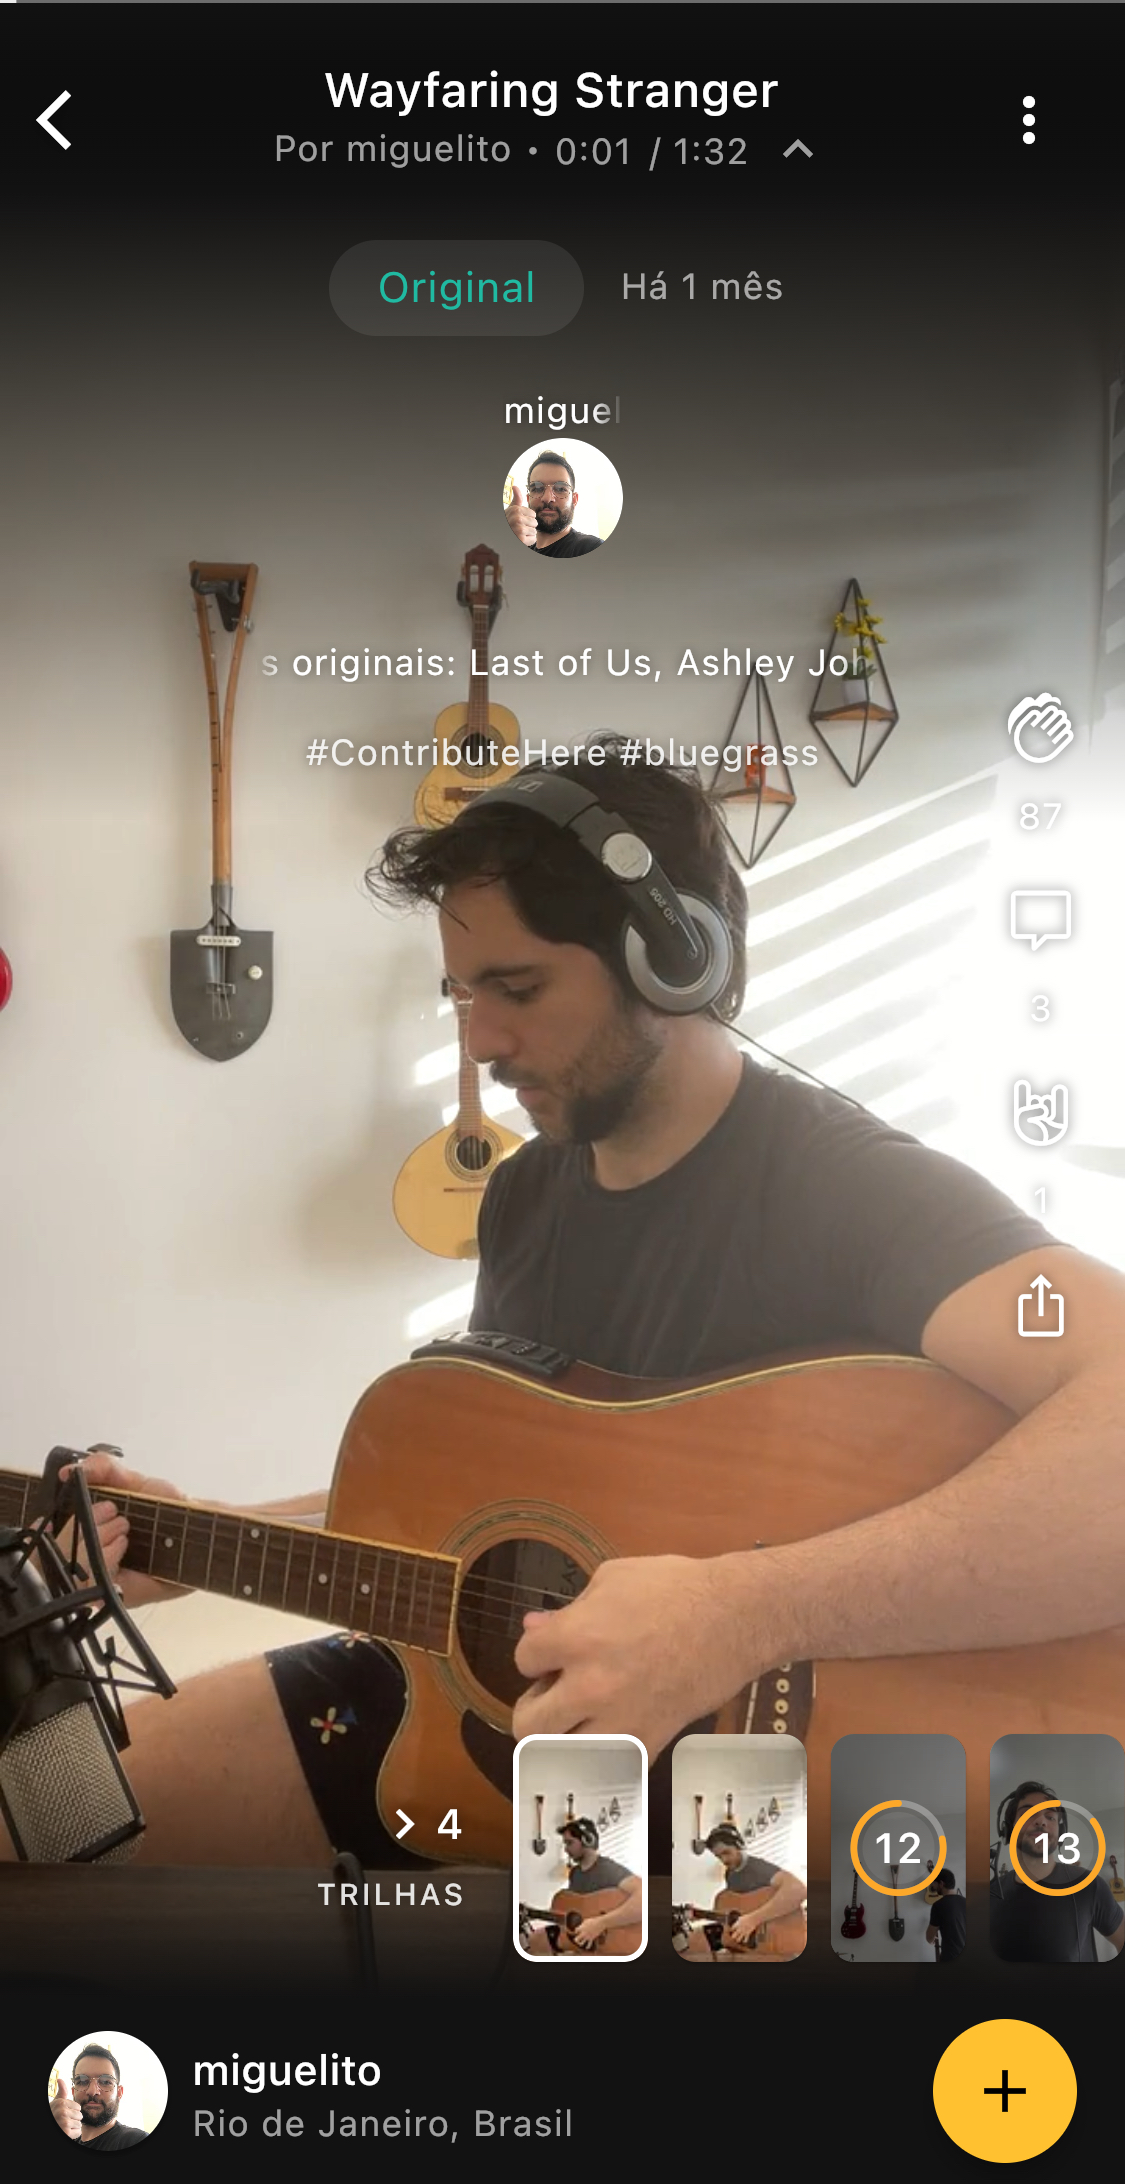
\includegraphics[width=0.4\textwidth]{chapters/chap02/images/wayfaring_original.jpeg}}
    \subfigure[]{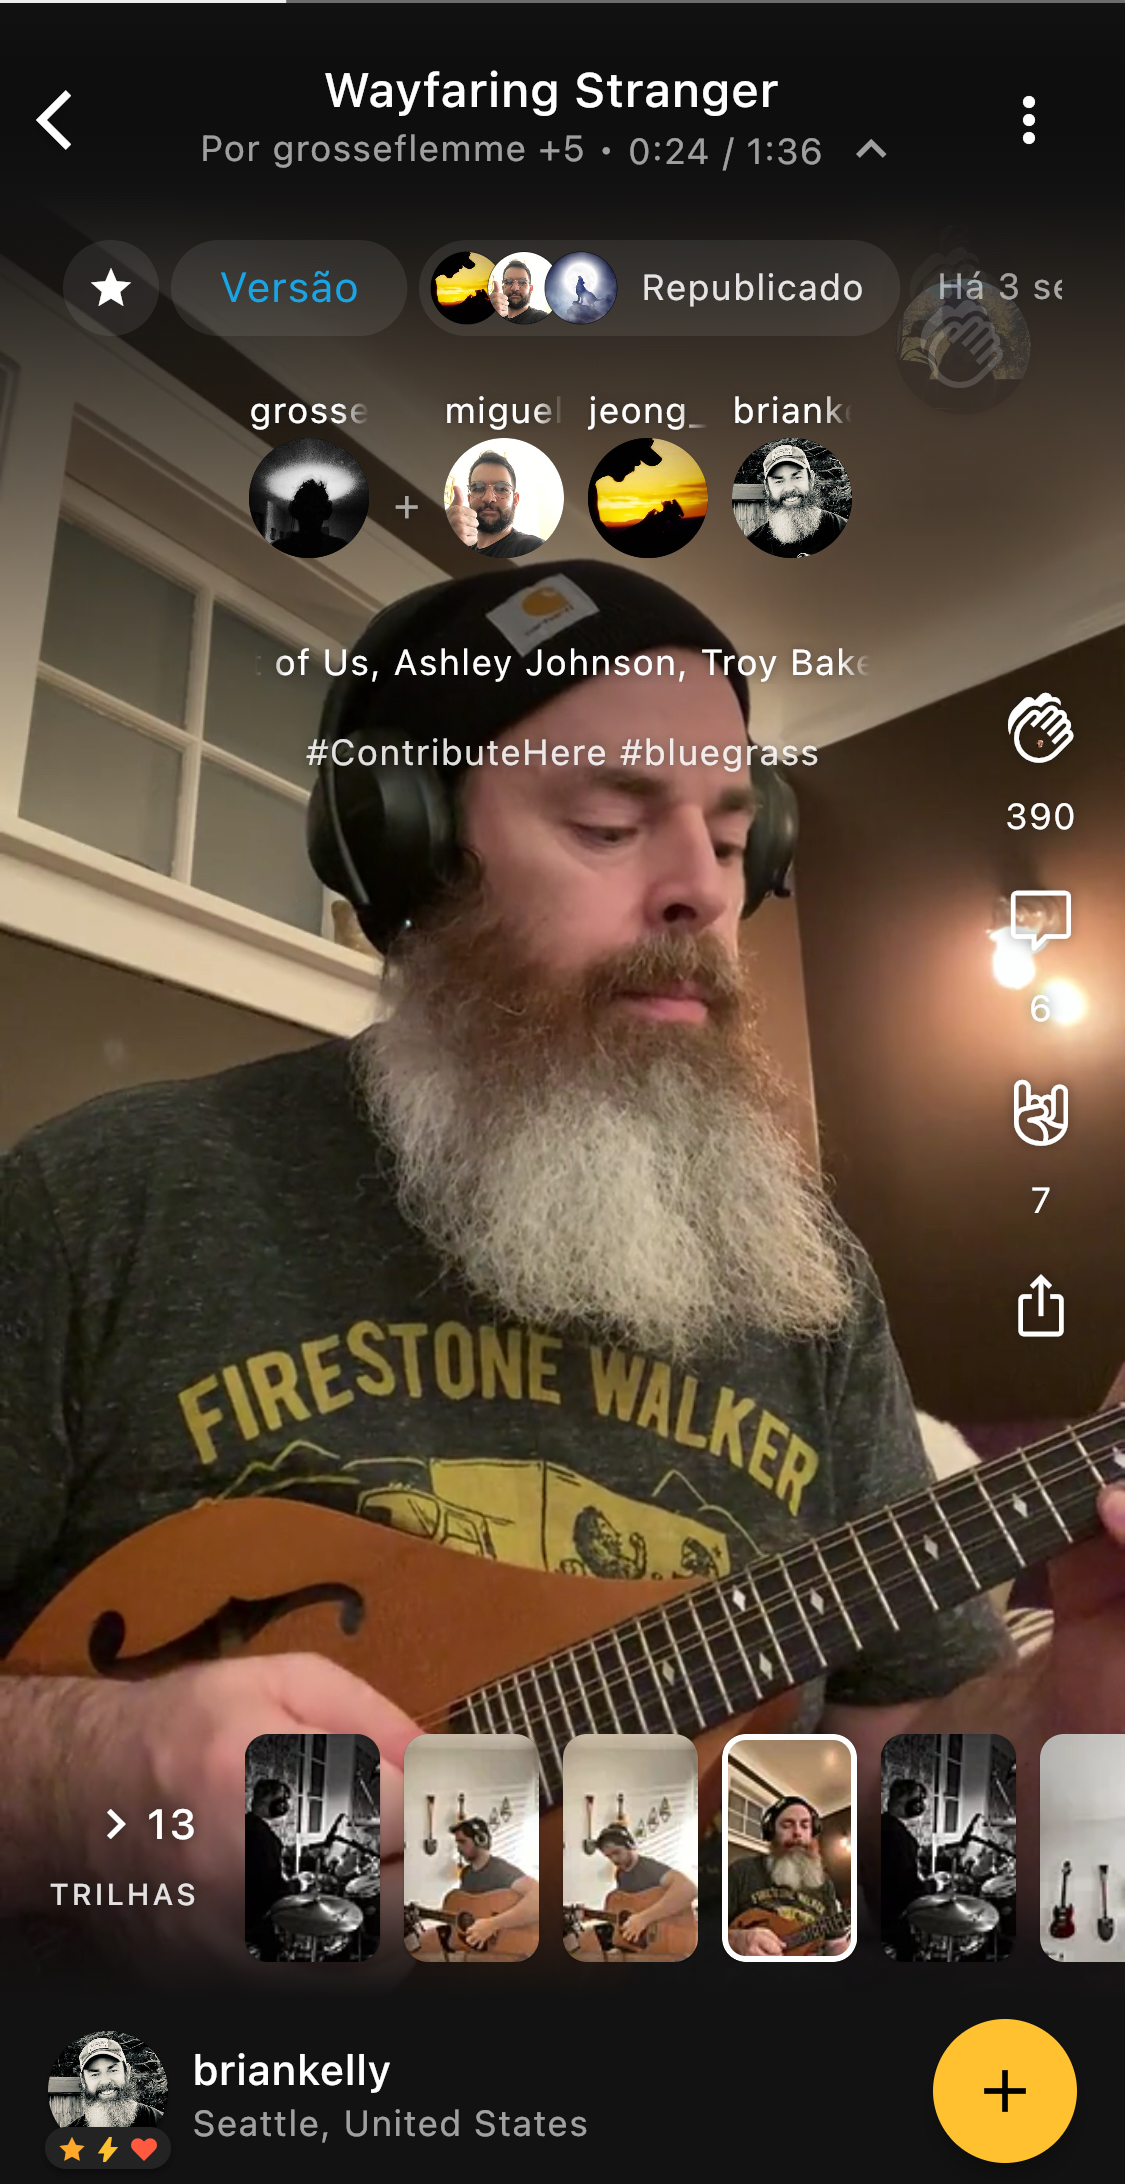
\includegraphics[width=0.4\textwidth]{chapters/chap02/images/wayfaring_fork.jpg}}
    \caption{Duas sessões publicadas no aplicativo Indaband. A primeira sessão é
    a sessão original, enquanto a segunda é um \textit{fork} subsequente da
    primeira. Ambas compartilham o mesmo nome e as faixas da primeira sessão. A
    segunda sessão contém faixas adicionais.}
    \label{fig:session_and_fork}
  \end{center}
  \end{figure}

\subsubsection{\textit{Fork}} Toda sessão publicada disponibiliza a
funcionalidade de \textit{fork} para os demais usuários da plataforma. O
\textit{fork} é uma cópia da sessão original, em que é possível adicionar
gravações inéditas, editar e remover faixas pré-existentes sem afetar a
publicação original. Quando publicada, a sessão \textit{fork} exibe o autor original das faixas
pré-existentes que forem mantidas, além da referência para a sessão anterior.

O \textit{fork} é uma das principais formas de colaboração assíncrona entre
usuários. A FIGURA \ref{fig:session_and_fork} ilustra duas sessões, sendo a
segunda um \textit{fork} subseqeuente da primeira. Note que a quantidade de
faixas e usuários presentes na segunda sessão aumenta. Além disso, conta com
maior quantidade de visualizações, comentários e outras formas de engajamento
positivo. Entre essas duas sessões, houve uma série de \textit{forks}
intermediários, realizados por cada um dos usuários que adicionaram faixas às
suas sessões.


\subsubsection{Faixa}
A faixa é uma mídia com áudio e vídeo que geralmente contém a gravação de um
instrumento ou voz. Uma faixa necessariamente é criada a partir de um entre três
recursos: tal como uma gravação original, tal como um \textit{fork} de uma faixa
publicada anteriormente ou como uma importação de uma mídia de áudio ou de
vídeo.




\section{Sobrecarga de informação}

Após três anos de desenvolvimento, a aplicação conta com dezenas de milhares de
usuários cadastrados, os quais centenas gravam mensalmente. Dado o grande
catálogo de usuários, o processo de encontrar pessoas com interesses musicais
similares demanda tempo e esforço. O mesmo ocorre ao procurar uma sessão que
seja de interesse em meio ao grande volume de conteúdo publicado. Essa
dificuldade percebida pelo usuário é conhecida na literatura de sistemas de
recomendação como sobrecarga de informação \cite{roetzel2019information}.

A sobrecarga de informação, segundo \citet{roetzel2019information}, é um estado em que um tomador de decisões observa um
conjunto ou uma carga de informações de complexidades distintas, a qual inibe a
capacidade do tomador de decisões de determinar de forma ótima a melhor decisão
possível.

\vspace{0.2cm}
\begin{figure}[h]
    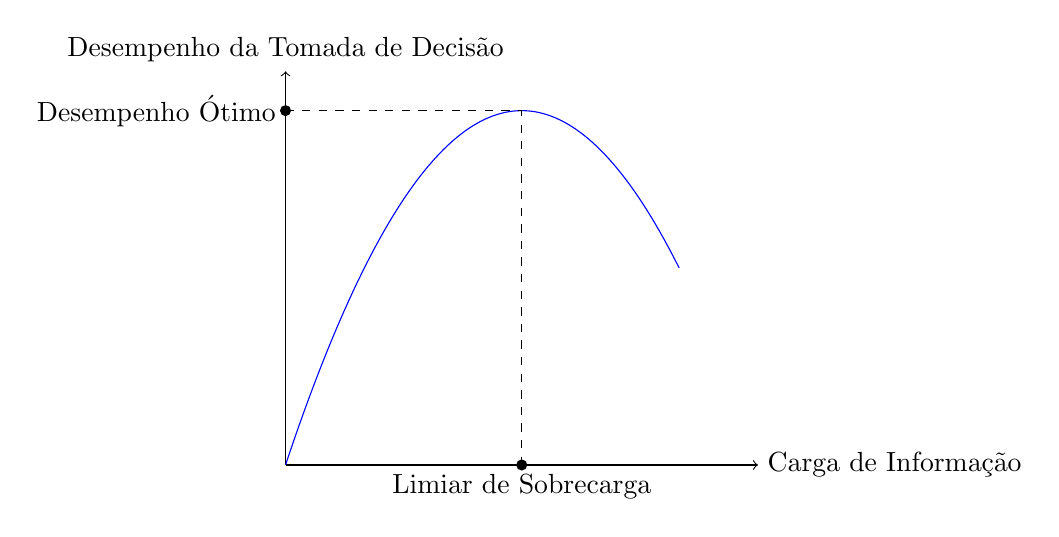
\begin{tikzpicture}
    % Eixo X
    \draw[->] (0,0) -- (6,0) node[right] {Carga de Informação};
    % Eixo Y
    \draw[->] (0,0) -- (0,5) node[above] {Desempenho da Tomada de Decisão};
  
    % Curva U invertida
    \draw[blue, domain=0:5, samples=100] plot (\x, {3*\x - 0.5*\x*\x});
  
    % Pontos de interesse
    \fill (0,4.5) circle (2pt) node[left] {Desempenho Ótimo};
    \fill (3,0) circle (2pt) node[below] {Limiar de Sobrecarga};

    % Linhas tracejadas
    \draw[dashed] (0,4.5) -- (3,4.5);
    \draw[dashed] (3,0) -- (3,4.5);
  \end{tikzpicture}
   % Descrição
    \caption{Correspondência entre a carga de informação e o desempenho da tomada
    de decisão.}
    \label{fig:u_invertida}
\end{figure}
\vspace{0.2cm}

O uso subótimo de informações é causado
pela limitação de recursos individuais escassos. Um recurso escasso pode ser uma
característica individual (como capacidade de processamento em série, memória de
curto prazo) ou equipamento relacionado à tarefa (por exemplo, orçamento ou
tempo para tomar uma decisão). A probabilidade de alcançar a melhor decisão
possível é definida como o desempenho de tomada de decisão. A correspondência
entre a carga de informação e o desempenho da tomada de decisão é ilustrada na
FIGURA \ref{fig:u_invertida} \cite{roetzel2019information}.

Experimentos realizados por \citet{liang2006personalized} mostraram que, ao
avaliar a satisfação de voluntários com um sistema de recomendação de notícias,
a precisão do conteúdo recomendado e o número de itens
recomendados influenciam diretamente na satisfação do usuário, reduzindo a
sobrecarga de informação e a insatisfação gerada pela sobrecarga.

\section{Sistemas de Recomendação}

\abbrev{RS}{sistemas de recomendação}
Sistemas de recomendação (RS, do inglês \textit{recommender systems}) são
ferramentas de \textit{software} que sugerem itens úteis para um usuário, de
acordo com a disponibilidade de seu histórico \cite{ricci2010introduction}. Esses
sistemas, que podem ser personalizados ou não-personalizados, ajudam usuários a
lidarem com processos de tomada de decisão em meio a sobrecarga de informações,
seja na escolha de um produto em um \textit{e-commerce} ou na seleção de um
filme em um serviço de \textit{streaming}. Ao contrário de uma ferramenta de
busca em que o usuário ativamente procura por um item específico, sistemas de
recomendação são úteis quando o usuário explora um catálogo diversificado,
otimizando a distribuição dos itens a partir de suas preferências pessoais. As
FIGURAS \ref{fig:spotify} e \ref{fig:twitter} ilustram sistemas de recomendação
para tarefas distintas: recomendação de \textit{playlists} na plataforma Spotify
e recomendação de perfis de usuário na plataforma Twitter, respectivamente.


\begin{figure}[ht]
    \centering
    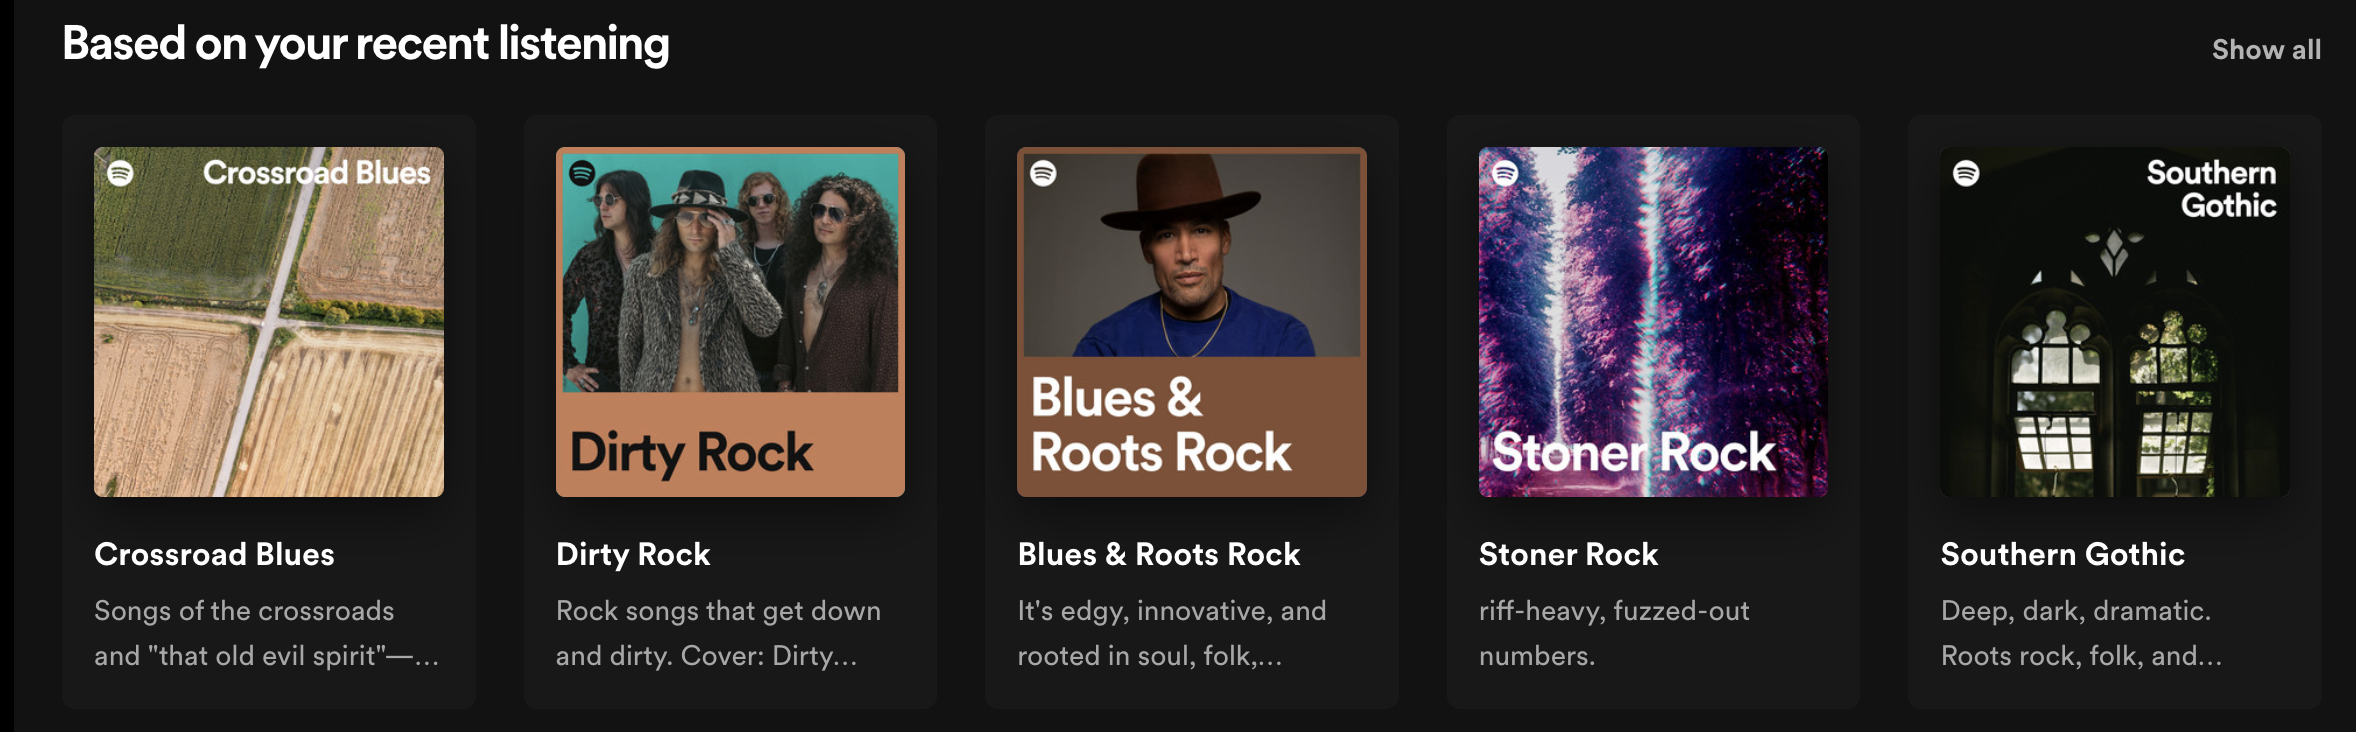
\includegraphics[width=0.8\textwidth]{chapters/chap01/images/spotify.png}
    \caption{Recomendações de \textit{playlists} no Spotify em Agosto de 2023.}
    \label{fig:spotify}
\end{figure}


Personalização é o processo de coleta e uso de informações pessoais para filtrar
conteúdo de forma única a um usuário, atendendo suas necessidades percebidas
pelo serviço ou declaradas explicitamente. \cite{liang2006personalized}.
Recomendações não-personalizadas distribuem o conteúdo recomendado de maneira
igualitária para todos os usuários, desconsiderando suas preferências
individuais. Uma recomendação a partir da lista de reportagens mais lidas em um
portal de notícias é um exemplo de recomendação não-personalizada.
\cite{falk2019practical}.

\begin{figure}[ht]
    \centering
    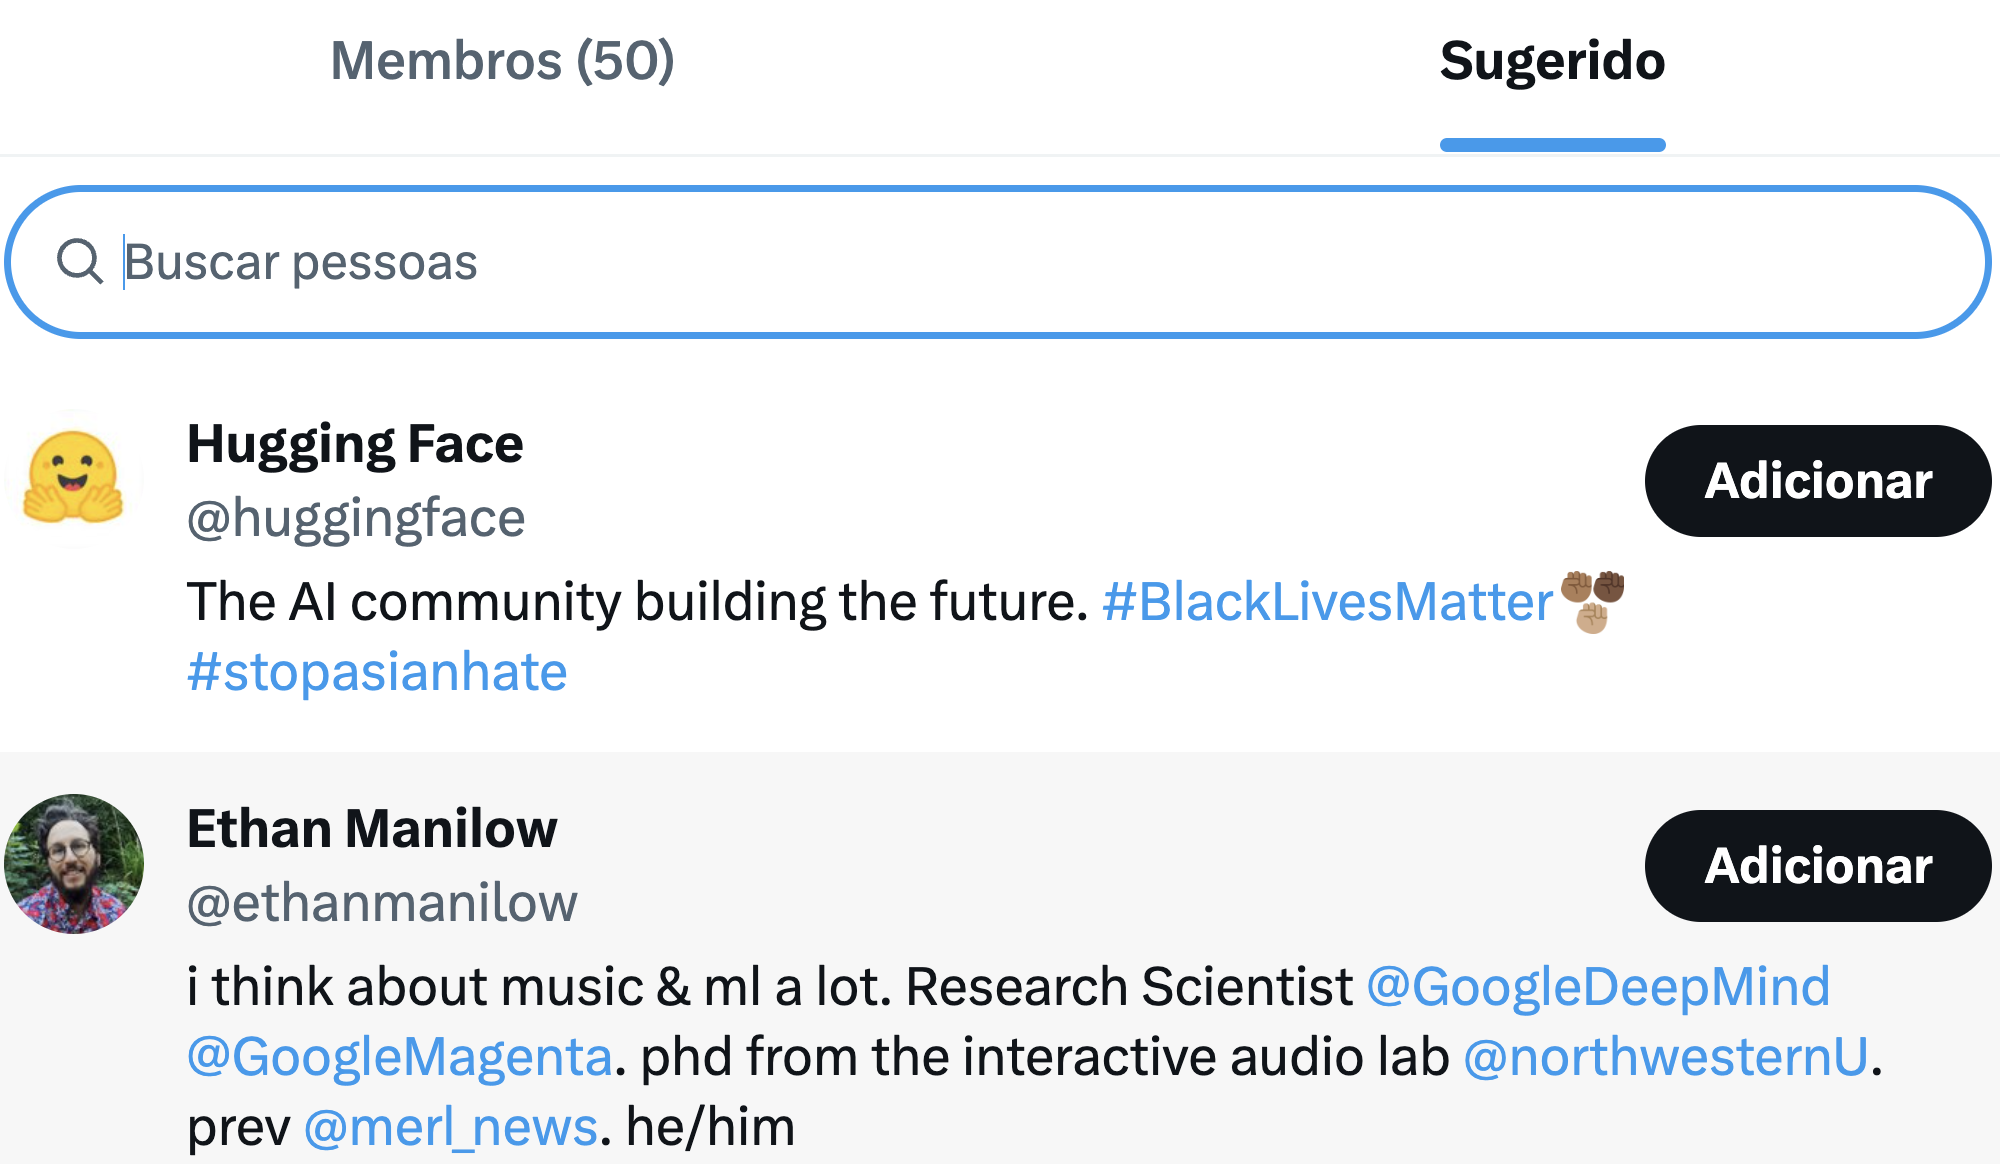
\includegraphics[width=0.6\textwidth]{chapters/chap01/images/tt.png}
    \caption{Recomendações de perfis de usuário no Twitter em Agosto de 2023.}
    \label{fig:twitter}
\end{figure}

% Sistemas de Recomendação Baseados em Sessão (SBRS, do inglês
% \textit{session-based recommender systems}) são sistemas de recomendação que 
Abordagens mais tradicionais em sistemas de recomendação modelam as interações
usuário-item na forma de uma matriz esparsa de avaliações. Cada linha da matriz
representa um usuário e cada coluna representa um item.

A tarefa em questão se
resume ao preenchimento dos valores faltantes da matriz, a depender da
abordagem escolhida. Valores preenchidos com avaliações altas são recomendados
ao usuário, uma vez que ele ainda não os consumiu, tal como ilustrado
na FIGURA \ref{fig:matriz_15}.


\begin{figure}[h]
    \centering
    \begin{tikzpicture}
        % Define the matrix
        \matrix (m) [matrix of nodes,
                    %  nodes in empty cells,
                     column sep=-\pgflinewidth,  % Adjust cell spacing
                     row sep=-\pgflinewidth,     % Adjust cell spacing
                     nodes={draw, text width=2.5em, align=center, minimum height=2.5em, minimum width=2.5em}] {
            5 & 4 & 1 & 1 \\
            4 & 4 & 1 & 1 \\
            1 & 2 &  & 4 \\
            1 & 1 & 4 & 4 \\
        };
      
        % % Labels on the left
        \foreach \row/\label in {1/Gilberto, 2/Maria, 3/Gal, 4/Caetano} {
          \node[left] at (m-\row-1.west) {\label};
        }
      
        % % Labels on the top
        \foreach \col/\label in {1/TV, 2/DVD, 3/sal, 4/pipoca} {
          \node[above,
          ] at (m-1-\col.north) {\label};
        }
      \end{tikzpicture}
      \caption{Matriz de avaliações para produtos de um comércio eletrônico. A predição atua sobre as avaliações não preenchidas.}
      \label{fig:matriz_15}
\end{figure}

\abbrev{SBRS}{Sistemas de recomendação baseados em sessão}
Por mais que a matriz de avaliações seja uma forma intuitiva de representação,
viabilizando uma boa variedade de modelos, trata-se de uma forma que
desconsidera o contexto temporal das interações ou a sequência específica de
itens que determinado usuário interagiu. Sistemas de Recomendação Baseados em
Sessão (SBRS, do inglês \textit{session-based recommender systems}) atuam
justamente nesse cenário.

Os SBRS se caracterizam pelos seus dados representarem um conjunto delimitado de
interações obtidas por \textit{feedback} implícito, ou seja, por preferências
indiretas identificadas a partir de ações ou padrões de navegação. Essas interações
são agrupadas em conjuntos denominados sessões. Uma sessão pode conter uma sequência temporalmente
ordenada de ações executadas por um usuário, ou um conjunto de ações executadas
por um usuário anônimo sem uma ordem específica.

Os objetivos de um SBRS incluem
prever a próxima interação do usuário durante uma sessão em andamento,
recomendar o próximo item ou um conjunto de itens para uma sessão, ou ainda
recomendar uma sessão inteira \cite{domingues_large_2023, survey_wang_2021}.


    



\begin{figure}[h]
    \centering
        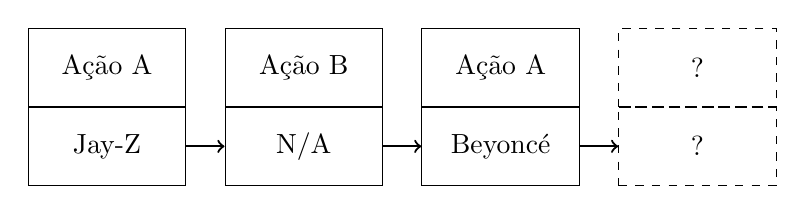
\begin{tikzpicture}
        % Draw the list cells
        \node[draw, rectangle, minimum width=2cm, minimum height=1cm] (cell1) at (0, 0) {Jay-Z};
        \node[draw, rectangle, minimum width=2cm, minimum height=1cm] (cell2) at (2.5, 0) {N/A};
        \node[draw, rectangle, minimum width=2cm, minimum height=1cm] (cell3) at (5, 0) {Beyoncé};
        \node[draw, dashed, rectangle, minimum width=2cm, minimum height=1cm] (cell4) at (7.5, 0) {?};

        % Draw the arrow
        \draw[->, thick] (cell1.east) -- (cell2.west);
        \draw[->, thick] (cell2.east) -- (cell3.west);
        \draw[->, thick] (cell3.east) -- (cell4.west);

        % % Add label to the left of the first cell
        % \node[left] at (cell1.west) {Sessão 1};

        % Draw the top cells with actions
        \node[draw, rectangle, minimum width=2cm, minimum height=1cm] (topcell1) at (0, 1.0) {Ação A};
        \node[draw, rectangle, minimum width=2cm, minimum height=1cm] (topcell2) at (2.5, 1.0) {Ação B};
        \node[draw, rectangle, minimum width=2cm, minimum height=1cm] (topcell3) at (5, 1.0) {Ação A};
        \node[draw, dashed, rectangle, minimum width=2cm, minimum height=1cm] (topcell4) at (7.5, 1.0) {?};

    \end{tikzpicture}
    \caption{Exemplo de uma sessão em andamento.}
    \label{fig:sessao_beyonce}
\end{figure}

Cada interação das sessões está associada a tuplas que contém um ou mais dos
seguintes dados: a ação executada, o item alvo da ação, o instante em que a ação
foi executada e o usuário responsável pela ação. Por exemplo, uma sessão pode
representar uma lista ordenada de itens selecionados por um usuário anônimo, ou
uma lista de ações executadas por usuários de uma mesma sessão, sem que essas
ações estejam necessariamente atreladas cada uma a um item. Isso é um aspecto
útil dos SBRS, por prover recomendações em aplicações em que não há distinção
entre usuários, ou quando as preferências de longo prazo de um usuário novo da
plataforma não foram identificadas. A FIGURA \ref{fig:sessao_beyonce} ilustra um
exemplo de sessão em andamento, em que a ação A corresponde a navegar ao perfil
de determinado artista, enquanto que a ação B corresponde a criar uma
\textit{playlist} vazia. Nem toda ação é necessariamente associada a um item,
como expresso na Ação B.
\vspace{0.4cm}
\section{Trabalhos Futuros}
% TODO: @Miguel - Needs review

A bibliografia existente de espectrograma de modulação, até o presente momento,
aplica uma segunda STFT sobre o domínio acústico, com a finalidade de medir
oscilações de intensidade no eixo da frequência. Dessa forma, o novo eixo obtido
pelo espectrograma de modulação representa modulações de amplitude.

Considerando
que o espectrograma acústico reside em um espaço vetorial $\mathbb{R}_3$, uma proposta de trabalho futuro é
investigar a possibilidade de representar modulações em frequência, bastando que a segunda
STFT meça as oscilações no eixo da frequência para uma dada intensidade
constante.
% \section{Modelagem com inclusão de instrumento e gênero}
\subsection{Base restrita a faixas inéditas} 

Uma característica particular das sessões do Indaband é a capacidade de criar
uma sessão a partir de outra já existente, modificá-la, adicionar novas
gravações e publicá-la como uma nova iteração a partir da funcionalidade de
\textit{fork}.

Essa funcionalidade é muito utilizada pelos usuários. A tabela \ref{tab_sessoes}
mostra que 76\% das faixas criadas são geradas via \textit{fork},
independentemente se foram publicadas ou não. Dessa forma, usuários distintos
podem contribuir para uma mesma sessão em momentos distintos, ou um usuário pode
contribuir para uma mesma sessão de outro usuário que era desconhecido até
então.

Uma vez que o objetivo é recomendar usuários prováveis de contribuir gravando
uma faixa inédita para uma determinada sessão, é razoável gerar um cenário em
que o recomendador seja treinado e avaliado estritamente para prever a próxima
faixa inédita gravada.

As abordagens \textit{next-item} e \textit{remaining-items} são as mais
utilizadas nos comparativos publicados porque aproveitam todos os itens de cada
sessão para o treinamento ou para a avaliação. No caso de uma aplicação em que
haja redundância entre as sessões, em que usuários possam salvar, repetir e
compartilhar sessões entre si, essas abordagens acabam por facilitar o trabalho
do recomendador, uma vez que cada iteração a mais no processo de treinamento
significa uma nova oportunidade para minimizar o erro do modelo. O mesmo vale
para a avaliação, em que identificar faixas \textit{forkadas} seria em tese uma
tarefa mais fácil. O cenário mais desafiador é aquele em que o item a ser
avaliado é necessariamente um item inédito no contexto daquela sessão.

Em contraponto, a abordagem \textit{last-item} é a que mais se aproxima do
cenário mencionado, uma vez que mantém inalterada a sequência de itens das
sessões. O que muda é a forma de avaliação, que passa a considerar apenas o
último item da sequência como o item a ser previsto, sem que os demais itens
anteriores sejam avaliados, minimizando a influência de itens \textit{forkados}
na avaliação.

Com essa finalidade, a base de treinamento do presente trabalho é filtrada:
Nesse último experimento, constam apenas sessões em que o último item da
sequência é a adição de uma faixa inédita. Essa identificação é feita a partir
de um metadado disponível, informando se a faixa foi gerada por um \textit{fork}
ou foi criada, seja por gravação, por importação de uma faixa ou por separação
de fontes.

Para essa abordagem, é utilizado o avaliador \textit{last-item}. Esse avaliador
considera apenas o último item da sequência como o item a ser previsto, sem que
os demais itens advindos de \textit{fork} sejam recomendados.

\begin{table}[htbp]
    \begin{tabular}{|l|l|l|l|l|l|l|l|}
      \hline
      Modelo & HR@5 & HR@10 & MRR@5 & MRR@10 & Cov@10 & Pop@10  \\
      \hline
      GNN & \textbf{0,551} & \textbf{0,625} & \textbf{0,437} & \textbf{0,446} & 0,660 & 0,202  \\
      \hline
      $\text{STAMP}_1$ & 0,519 & 0,584 & 0,377 & 0,386 & 0,610 & 0,217 \\
      \hline
      sknn2 & 0,518 & 0,647 & 0,213 & 0,230 & 0,643 & 0,169 \\
      \hline
      sknn1 & 0,515 & 0,642 & 0,209 & 0,226 & 0,592 & 0,197 \\
      \hline
      ct & 0,509 & 0,579 & 0,390 & 0,399  & 0,477 & 0,349 \\
      \hline
      $\text{STAMP}_2$ & 0,506 & 0,590 & 0,366 & 0,377 & 0,609 & 0,201 \\
      \hline
      $\text{NextItNet}_2$ & 0,465 & 0,563 & 0,341 & 0,354 & 0,566 & 0,249 \\
      \hline
      $\text{STAN}_2$ & 0,464 & 0,596 & 0,178 & 0,196 & 0,547 & 0,179 \\
      \hline
      $\text{STAN}_1$ & 0,451 & 0,572 & 0,186 & 0,202 & 0,529 & 0,177 \\
      \hline
      $\text{NextItNet}_1$ & 0,449 & 0,536 & 0,337 & 0,349 & 0,525 & 0,257\\
      \hline
      vsknn1 & 0,447 & 0,580 & 0,1193 & 0,211 & 0,544 & 0,208 \\
      \hline
      $\text{VSTAN}_1$ & 0,441 & 0,580 & 0,180 & 0,198 & 0,507 & 0,221 \\
      \hline
      $\text{SMF}_2$ & 0,439 & 0,553 & 0,291 & 0,306 & 0,306 & 0,240 \\
      \hline
      $\text{SMF}_1$ & 0,431 & 0,530 & 0,298 & 0,311 & 0,240 & 0,257 \\
      \hline
      vsknn2 & 0,427 & 0,564 & 0,172 & 0,190 & 0,618 & 0,163 \\
      \hline
      $\text{SR}_2$ & 0,423 & 0,534 & 0,277 & 0,291 & 0,471 & 0,238 \\
     \hline
      $\text{VSTAN}_2$ & 0,418 & 0,546 & 0,171 & 0,189 & 0,588 & 0,142 \\
      \hline
      $\text{SR}_1$ & 0,410 & 0,512 & 0,279 & 0,292 & 0,445 & 0,259 \\
      \hline
      ar & 0,395 & 0,498 & 0,248 & 0,262 & 0,454 & 0,265 \\
      \hline 
      $\text{NARM}_1$ & 0,361 & 0,455 & 0,229 & 0,241 & 0,658 & 0,199 \\
      \hline
      $\text{NARM}_2$ & 0,324 & 0,440 & 0,211 & 0,226 & 0,665 & 0,188 \\
      \hline
      FOSSIL & 0,287 & 0,420 & 0,137 & 0,154 & 0,776 & 0,249 \\
      \hline
      FPMC & 0,281 & 0,419 & 0,124 & 0,143 & 0,764 & 0,241 \\
      \hline
      FISM & 0,275 & 0,434 & 0,120 & 0,141 & 0,749 & 0,240 \\
      \hline
      BPRMF & 0,271 & 0,407 & 0,122 & 0,141 & 0,744 & 0,250 \\
      \hline
      CSRM & 0,264 & 0,343 & 0,158 & 0,168 & 0,596 & 0,137  \\ 
      \hline
      $\text{GRU4Rec}_2$ & 0,208 & 0,278 & 0,130 & 0,139 & 0,873 & \textbf{0,030}  \\
      \hline
      $\text{GRU4Rec}_1$ & 0,195 & 0,271 & 0,123 & 0,134 & \textbf{0,858} & 0,040  \\
      \hline
      rpop & 0,165 & 0,225 & 0,106 & 0,113 & 0,009 & 0,319 \\
      \hline
      pop & 0,127 & 0,242 & 0,083 & 0,098 & 0,006 & 0,530 \\
      \hline
      spop & 0,125 & 0,219 & 0,059 & 0,071 & 0,299 & 0,471 \\
      \hline
      random & 0,003 & 0,005 & 0,001 & 0,001 & 1,000 & 0,014 \\
      \hline
      \end{tabular}
      \label{tab:results_last_item_final}
    \caption{Resultado dos modelos \textit{session-based} na abordagem
    \textit{single item}, avaliando o último item da sessão. Modelos ordenados por HR@5. }
  \end{table}

  A tabela \ref{tab:results_last_item_final} mostra os resultados obtidos pela
  abordagem \textit{last-item}. As métricas obtiveram valores na mesma faixa da
  abordagem \textit{next-item}, demonstrando que, por mais que a avaliação e o
  treinamento seja reservados apenas ao último item da sequência, os modelos
  mantém desempenho equivalente.
  
  Novamente, o modelo GNN obteve os melhores resultados. Modelos
  mais simples, como o skNN e a árvore de contexto também obtiveram bons
  resultados.





\section{Filtragem de Modulação} \label{section_fil_mod}
A filtragem de modulação é uma técnica para filtragem de envoltórias com
oscilações lentas, presentes em sub-bandas de frequência, aplicada sobre sinais
não-estacionários.\cite{clark2009sum} \cite{li2005properties}. O objetivo, em
aplicações de fala, é obter um sinal mais inteligível na saída, composto apenas
pela composição de tons com modulações de baixa frequência associadas à
articulação vocal, eliminando as demais parcelas.

Essa técnica assume que um sinal $x[n]$ de valores reais é
representado pela soma dos produtos entre moduladora e portadora que compõem
cada sub-banda $x_k[n]$:
\begin{equation}
    x[n] = \sum_{k = 0}^{K - 1} x_k[n] = \sum_{k = 0}^{K - 1} m_k[n] c_k[n]
\end{equation}


A implementação genérica da filtragem de modulação está representada no diagrama de blocos abaixo.

\begin{figure}[h]
    \centering
    \begin{tikzpicture}[auto,>=latex']
        \tikzstyle{block} = [draw, shape=rectangle, minimum height=3em, minimum
        width=3em, node distance=4cm, line width=1pt]
        %Creating Blocks and Connection Nodes
        \node at (-2.5,0) (input) {$x[n]$};
        \node [block] (filterbank) {Banco de filtros};
        \node [block, right of=filterbank] (dem) {demodulação};
        \node [block, right of=dem] (LP) {passa-baixas};
        \node [block, below of = filterbank] (sintese) {síntese};
        \node [block, below of=dem] (res) {reconstrução};
        \node [left of=sintese, node distance=2.5cm] (output) {$x'[n]$};
        %Conecting Blocks
        \begin{scope}[line width=1pt]
            \draw[->] (input) -- (filterbank);
            \draw[->, line width=1mm] (filterbank) -- node[name=subband] {$x_k[n]$} (dem);
            \draw[->, line width=1mm] (dem) -- node[name=mod] {$m_k[n]$} (LP);
            \draw[->, line width=1mm] (dem) -- node[name=carrier] {$c_k[n]$} (res);
            \draw[->, line width=1mm] (LP) |- node[name=new_mod] {$m'_k[n]$} (res);
            \draw[->, line width=1mm] (res) -- node[name=new_subband] {$x'_k[n]$} (sintese);
            \draw[->] (sintese) -- (output);
        \end{scope}
    \end{tikzpicture}
    \caption{Filtro de modulação, em diagrama de blocos. Adaptado de \cite{li2005properties}.}
\end{figure}

O sinal banda-larga $x[n]$ passa por um banco de filtros, no qual as  $x_k[n]$
saídas do banco de filtros passam por um módulo de demodulação, no qual são
separadas as parcelas moduladoras $m_k[n]$ e portadoras $c_k[n]$ de cada
sub-banda. Cada parcela $m_k[n]$ é filtrada por um filtro passa-baixas, cuja
resposta ao impulso é $g[n]$. Em seguida, cada sub-banda é reconstruída a partir da portadora
$c_k[n]$ e da modulação filtrada $m'_k[n]$. Finalmente, o sinal de banda larga
$x'_k[n]$ é sintetizado com as sub-bandas $x'_k[n]$ reconstruídas, obtidas a
partir das modulações filtradas.

Em aplicações de \textit{Speech Enhancement}, o projeto do banco de filtros
emula a resposta em frequência da cóclea no sistema auditivo. Por sua vez, a
frequência de corte do filtro passa-baixas é tipicamente de 16Hz
\cite{drullman1994}, tal que frequências abaixo desse valor estão associadas às
periodicidades na construção de frases, palavras e sílabas.

Uma forma de calcular $m'_k[n]$ é a partir do espectro de modulação $P_k[\mu]$,
apresentado na equação \ref{modspec_filterbank}:

\begin{equation}
    m'_k[n] = g[n] \ast m_k[n] = \sum_{q = 0}^{n} g[n - q] m_k[q]
\end{equation}

\begin{equation}
    m'_k[n] = \sum_{\mu=0}^{N-1} G[\mu]P_k[\mu] e^{j \frac{2 \pi \mu}{N} n}
\end{equation}  \todo{janela na eq?}

Dessa forma, obtém-se $m'_k[n]$ a partir da transformada inversa do espectro de
modulação filtrado por $G[\mu]$ \cite{toolbox2010}.

\todo{specs de implementação}
\section{Materiais e Organização do Texto}

O trabalho proposto utiliza o \textit{framework} \textit{open-source}
session-rec \cite{sessionrec} escrito em Python, uma vez que contém uma ampla
variedade de modelos SBRS e métricas de avaliação, replicando o padrão de
pesquisas recentes sobre o tema. Os dados utilizados no trabalho foram cedidos
pela empresa Indaband, na condição de anonimização dos usuários tal como ordena
a Lei Geral de Proteção de Dados \cite{lgpd}. Os experimentos foram realizados
em uma máquina virtual com 12 GB de memória RAM, 75 GB de memória de
armazenamento e GPU NVIDIA Tesla T4.

O presente texto é organizado da seguinte forma: o segundo capítulo introduz a
base teórica e aborda diferentes sistemas de recomendação de forma abrangente,
apresentando as abordagens mais tradicionais e que sustentam a intuição de
modelos mais sofisticados do comparativo. A definição formal das recomendações
\textit{session-based} e \textit{session-aware} é apresentada, além de suas propriedades
e medidas de avaliação. Também é apresentada a base teórica de modelos de redes
neurais que constam nas arquiteturas dos sistemas de recomendação mais sofisticados,
cujas arquiteturas são descritas no mesmo capítulo.


O terceiro capítulo apresenta os comparativos realizados em abordagens
distintas. Os experimentos são feitos a partir do conjunto de dados do
aplicativo Indaband, e incluem os resultados das métricas de desempenho.


O quarto e último capítulo apresenta uma análise e avaliação dos resultados
obtidos a partir dos experimentos realizados. Também apresenta a proposta de
trabalhos futuros considerando os resultados da presente pesquisa.


  %%________________________

   %%________________________
  %% CHAPTER 05
  \chapter{Conclusōes}
\section{Indaband}
A música, enquanto atividade e produto, permite o estabelecimento de laços sociais
entre musicistas e ouvintes.

A atividade musical permite que um conjunto de musicistas interaja e
comunique-se, facilitada quando os membros compartilham de uma mesma bagagem
cultural. Além disso, permite que a audiência estabeleça um vínculo com
o músico executor ou o conjunto de musicistas \cite{cook2021music}.

Por sua vez, a música enquanto produto permite o estabelecimento de laços sociais
entre os ouvintes, seja em uma sala de concerto no século XIX, em uma sala de estar
com um rádio ou um gramofone no século XX, ou em uma apresentação ao vivo na
plataforma Twitch no século XXI.

Durante a pandemia de COVID-19, estudantes de música precisaram adaptar seus
hábitos de prática musical para aulas remotas e práticas individuais. A prática
coletiva foi fortemente afetada, uma vez que as aulas e os ensaios presenciais
foram suspensos em uma série de instituições de ensino, dado o risco de
contaminação e a necessidade de distanciamento social \cite{nusseck2021musical}.

A prática remota síncrona, hoje, enfrenta uma série de desafios técnicos. A
latência entre os praticantes é o principal problema. O limiar da percepção
auditiva para atrasos é de cerca de 20 milissegundos, enquanto que sistemas VoIP
com latência de 150 milissegundos e \textit{jitter} de 30 milissegundos são
considerados de boa qualidade. A codificação associada à compressão do sinal e a
largura de banda também influenciam no atraso. Enquanto a latência em uma
comunicação instantânea não for inferior ao limiar da percepção, essa forma de
prática musical não será viável.

A principal alternativa é a prática musical colaborativa assíncrona. Nesse
cenário, cada praticante grava sua faixa de forma individual enquanto ouve as
demais faixas gravadas. Aplicações como \textit{BandLab}, \textit{Ableton Live}
e \textit{Soundtrap by Spotify} funcionam sob essa abordagem.

Uma segunda característica da prática musical coletiva, seja no contexto
presencial ou remoto, é a necessidade de encontrar outros interessados com
gostos musicais similares, instrumentos que se complementem, etc. Uma pessoa que
deseja tocar um estilo musical específico, incomum na região em que vive,
sofreria dessa dificuldade. Um meio de resolver esse problema é recorrer à
comunidades virtuais ou redes sociais. Ao encontrar outros interessados, caso a
distância impeça a prática presencial, a atividade pode ser realizada a partir
da prática musical colaborativa assíncrona. Plataformas como \textit{Cifra Club}
e \textit{Ultimate Guitar} permitem que usuários contribuam com tablaturas de
músicas e comentários, formando uma comunidade virtual.


Tanto a prática musical colaborativa assíncrona quanto a formação de comunidades
virtuais de música são problemas os quais o mercado oferece poucas soluções
integradas. Estações de trabalho de áudio digital (DAWs, do inglês
\textit{Digital Audio Workstations}) mais tradicionais, como \textit{Pro Tools},
\textit{Logic Pro} e \textit{Ableton Live} são desprovidos de funcionalidades de
interação social. \textit{Cifra Club} e \textit{Ultimate Guitar} não permitem a
gravação colaborativa de forma assíncrona. \textit{Soundtrap by Spotify} e
\textit{BandLab} permitem a edição colaborativa em tempo real, porém apenas o
último contém funcionalidades de interação e integração social entre usuários. A
aplicação \textit{Collab}, da Meta, preenchia parcialmente esses critérios antes
de ser descontinuada. O aplicativo móvel Indaband foi criado para ocupar esse
espaço pouco preenchido no mercado.

\begin{figure}[h]
    \centering
    \subfigure[]{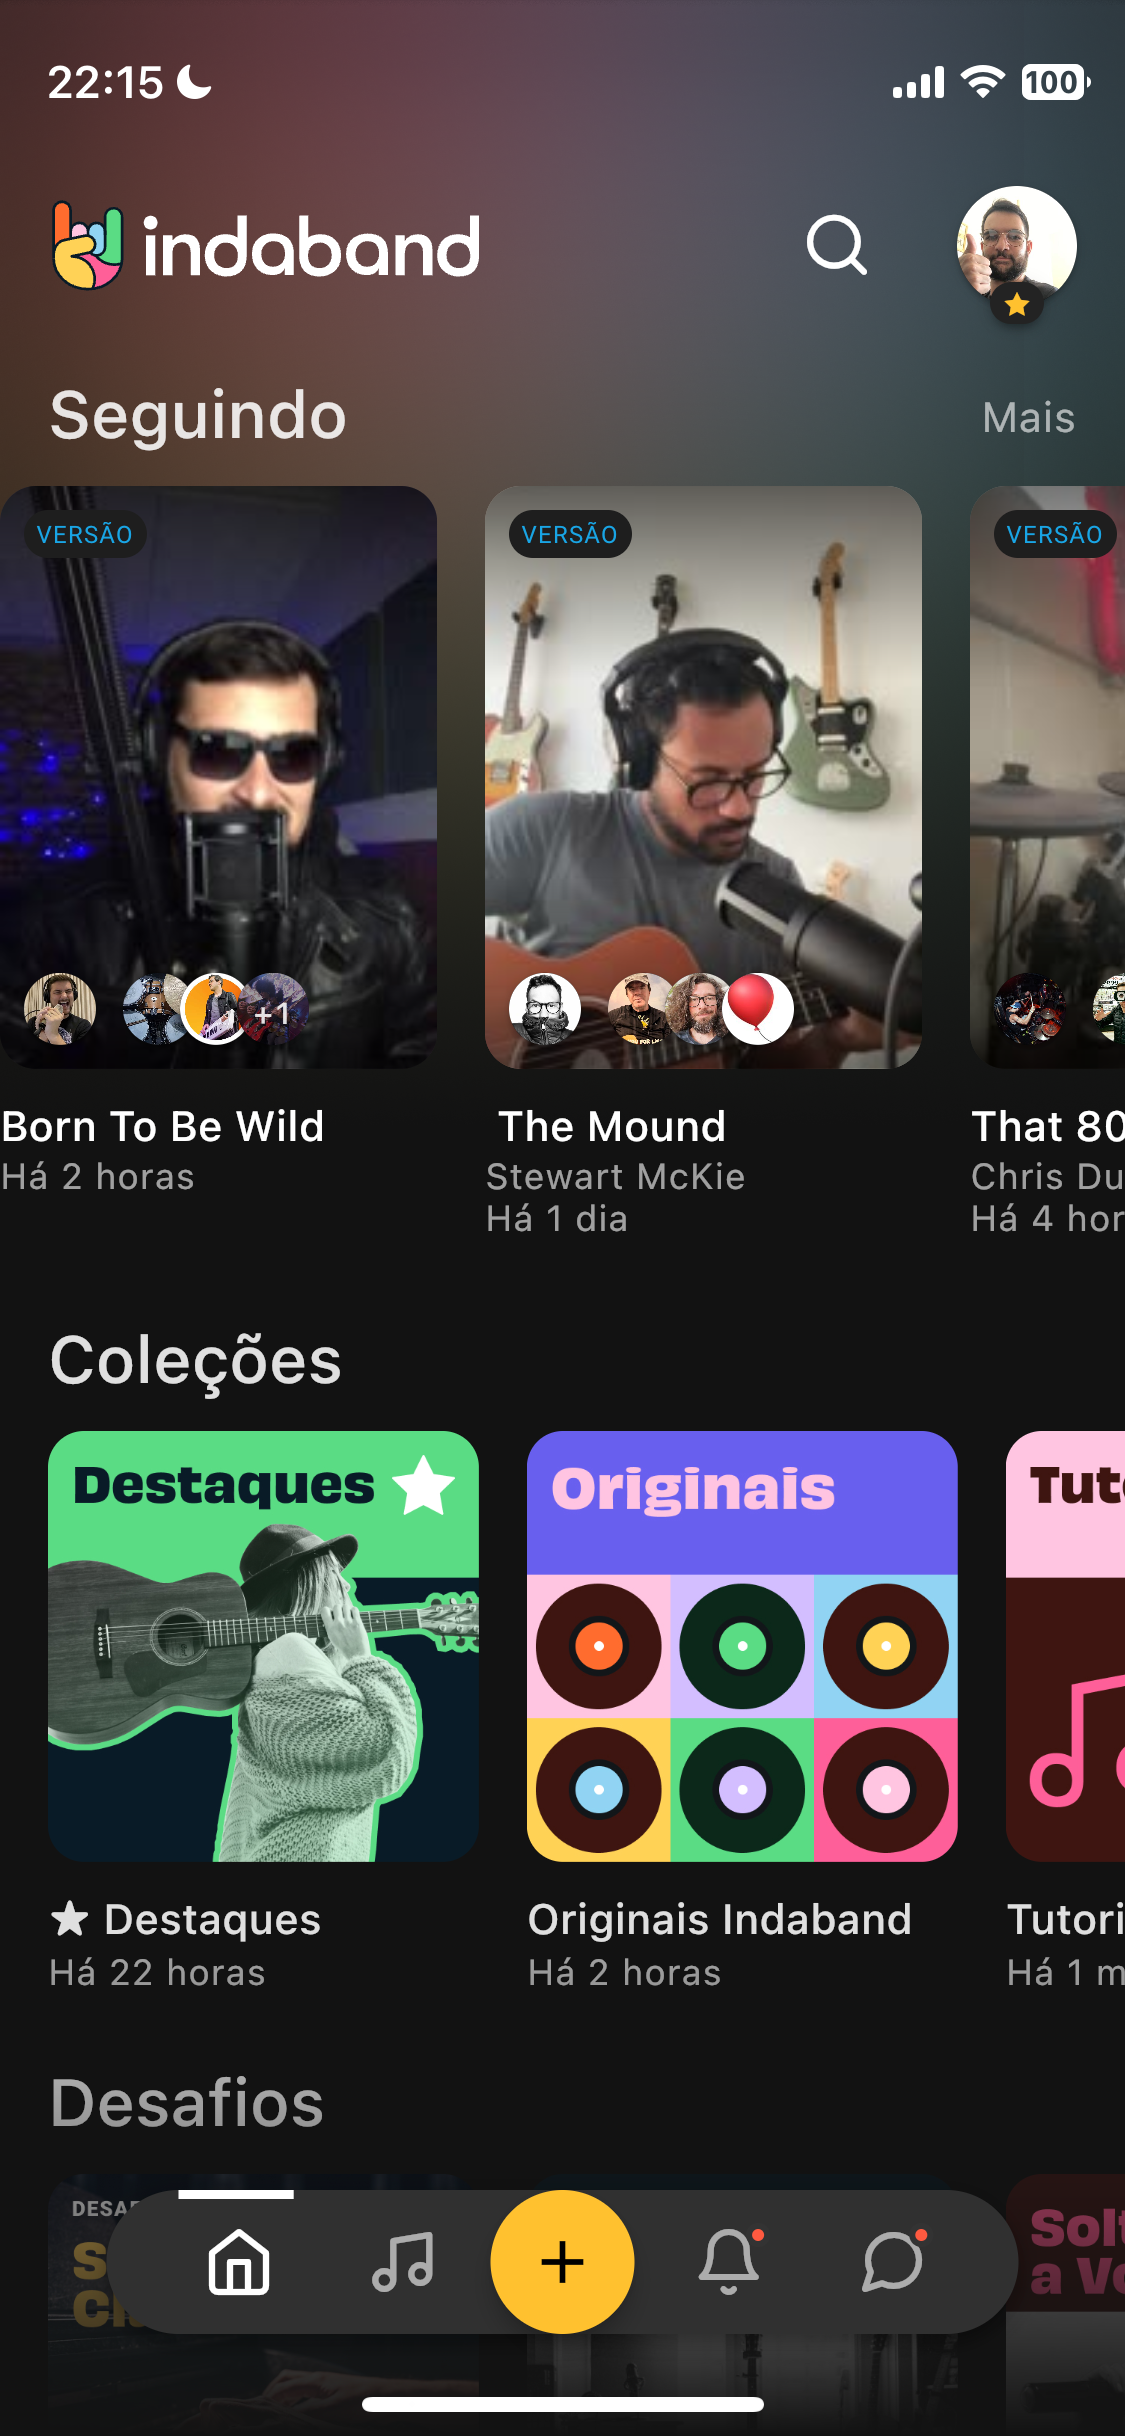
\includegraphics[width=0.24\textwidth]{chapters/chap01/images/inda/inda3.PNG}}
    \subfigure[]{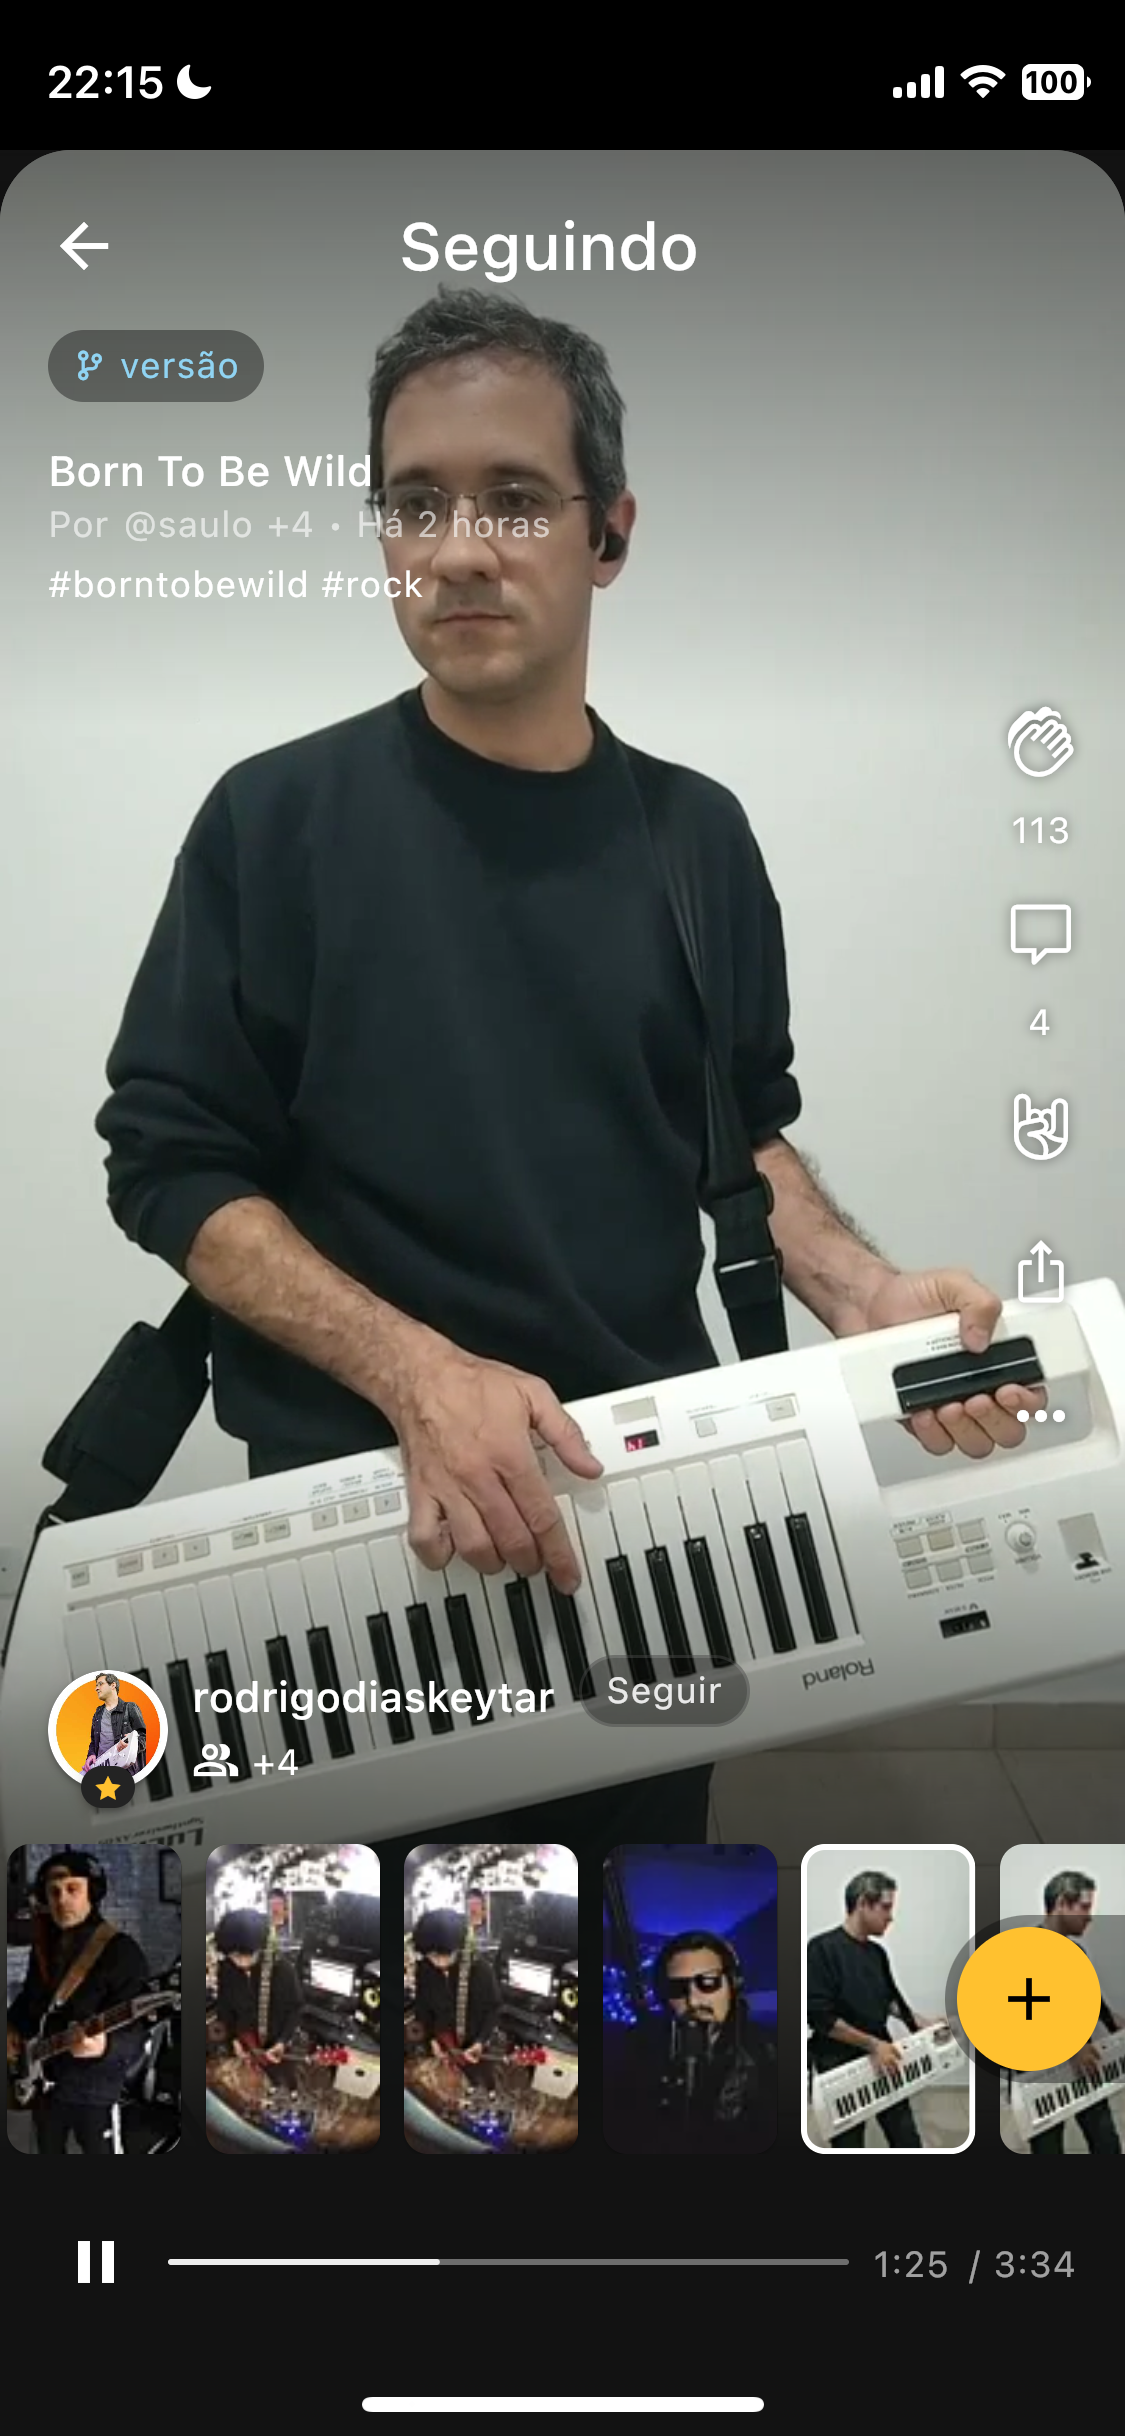
\includegraphics[width=0.24\textwidth]{chapters/chap01/images/inda/inda.PNG}}
    \subfigure[]{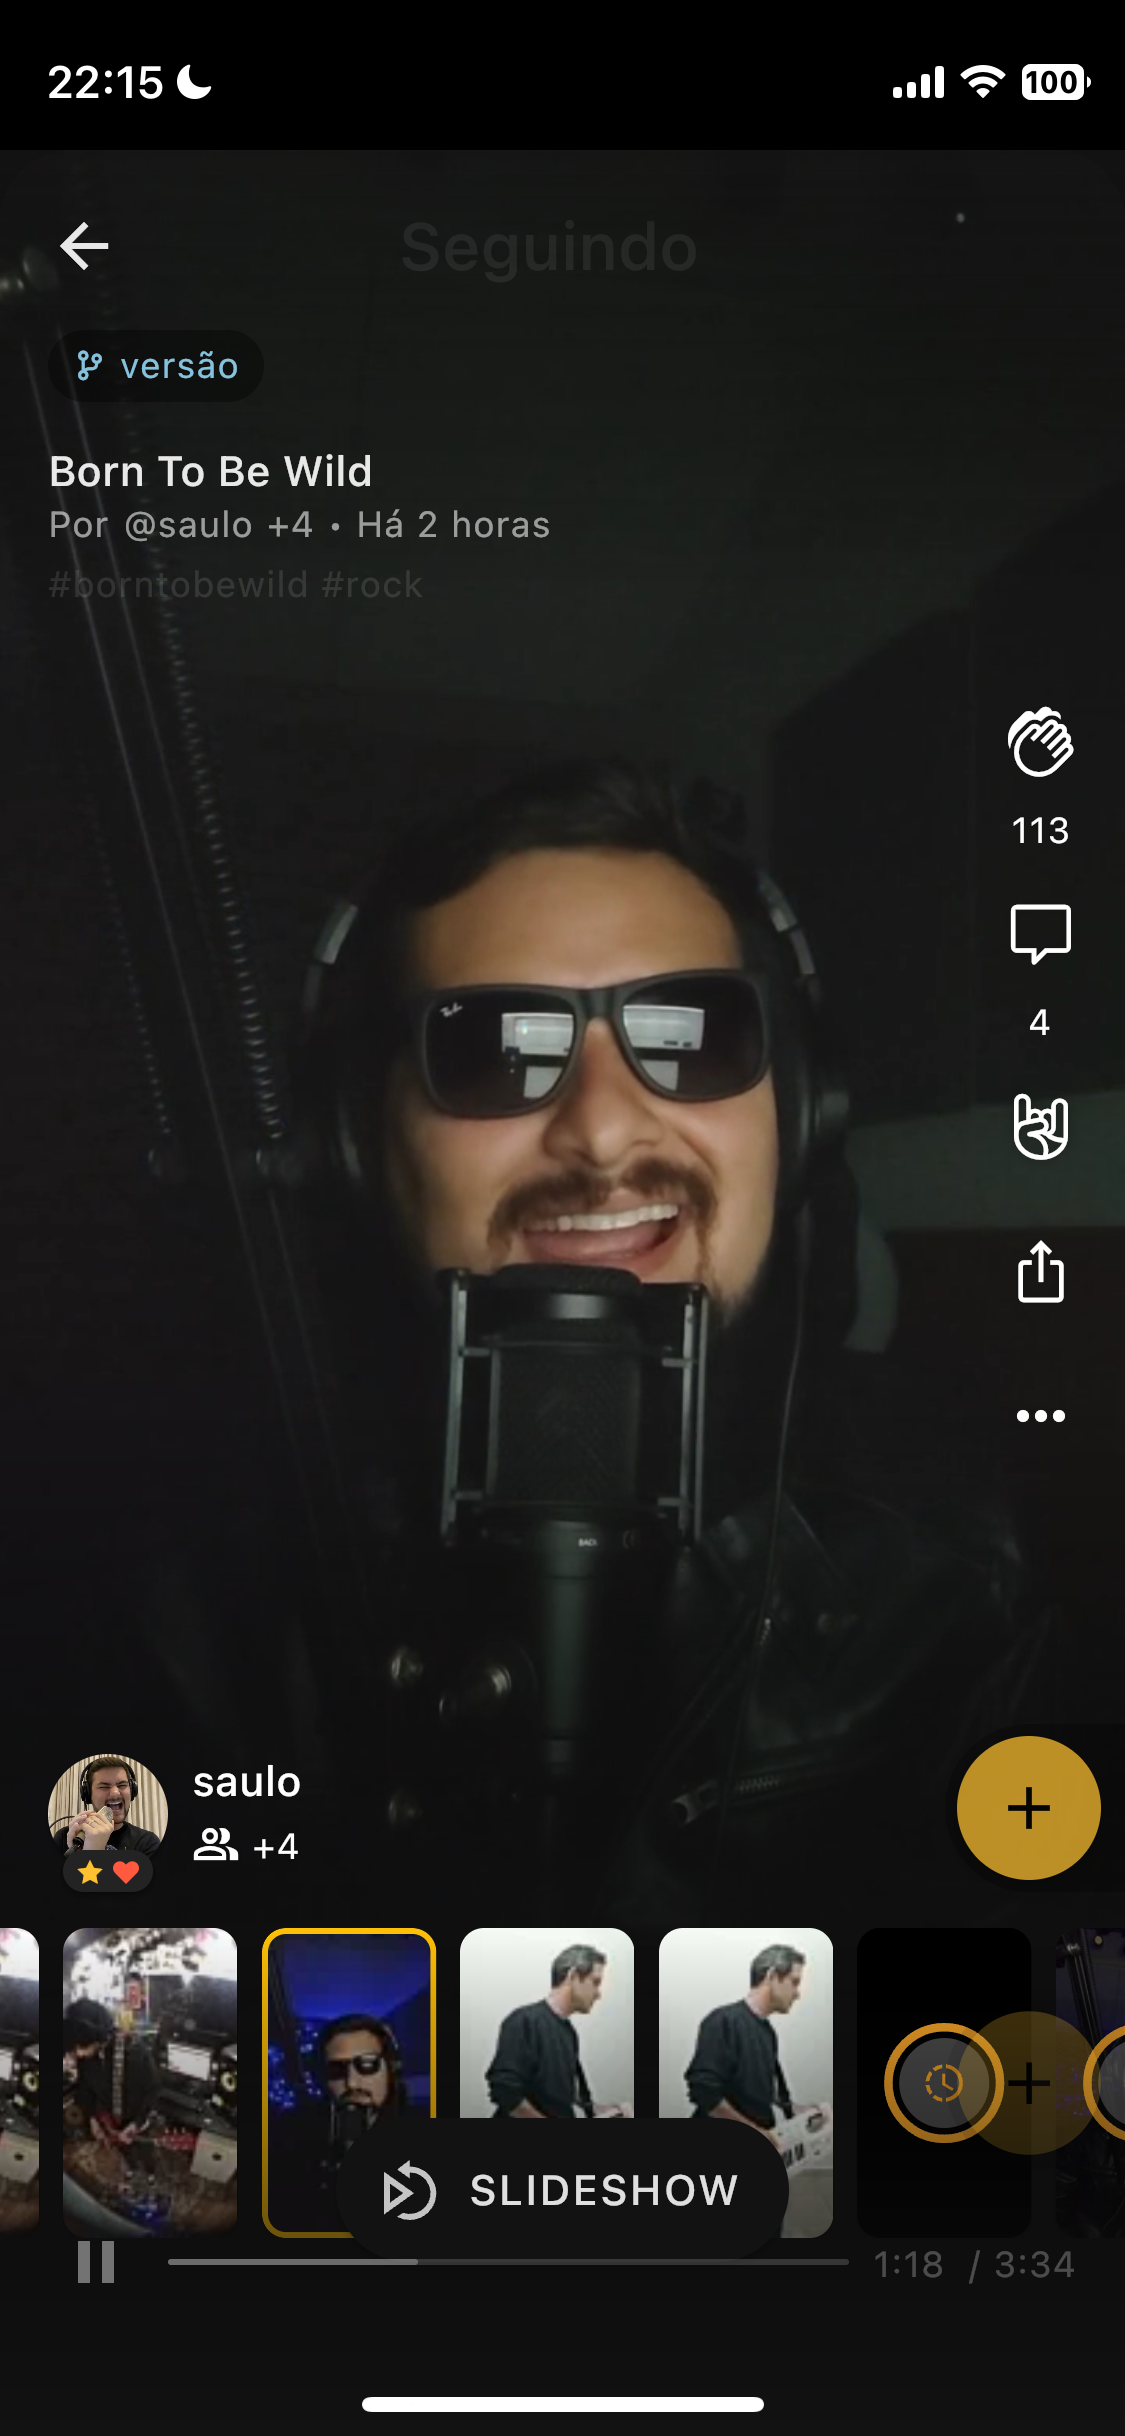
\includegraphics[width=0.24\textwidth]{chapters/chap01/images/inda/inda2.PNG}}
    \subfigure[]{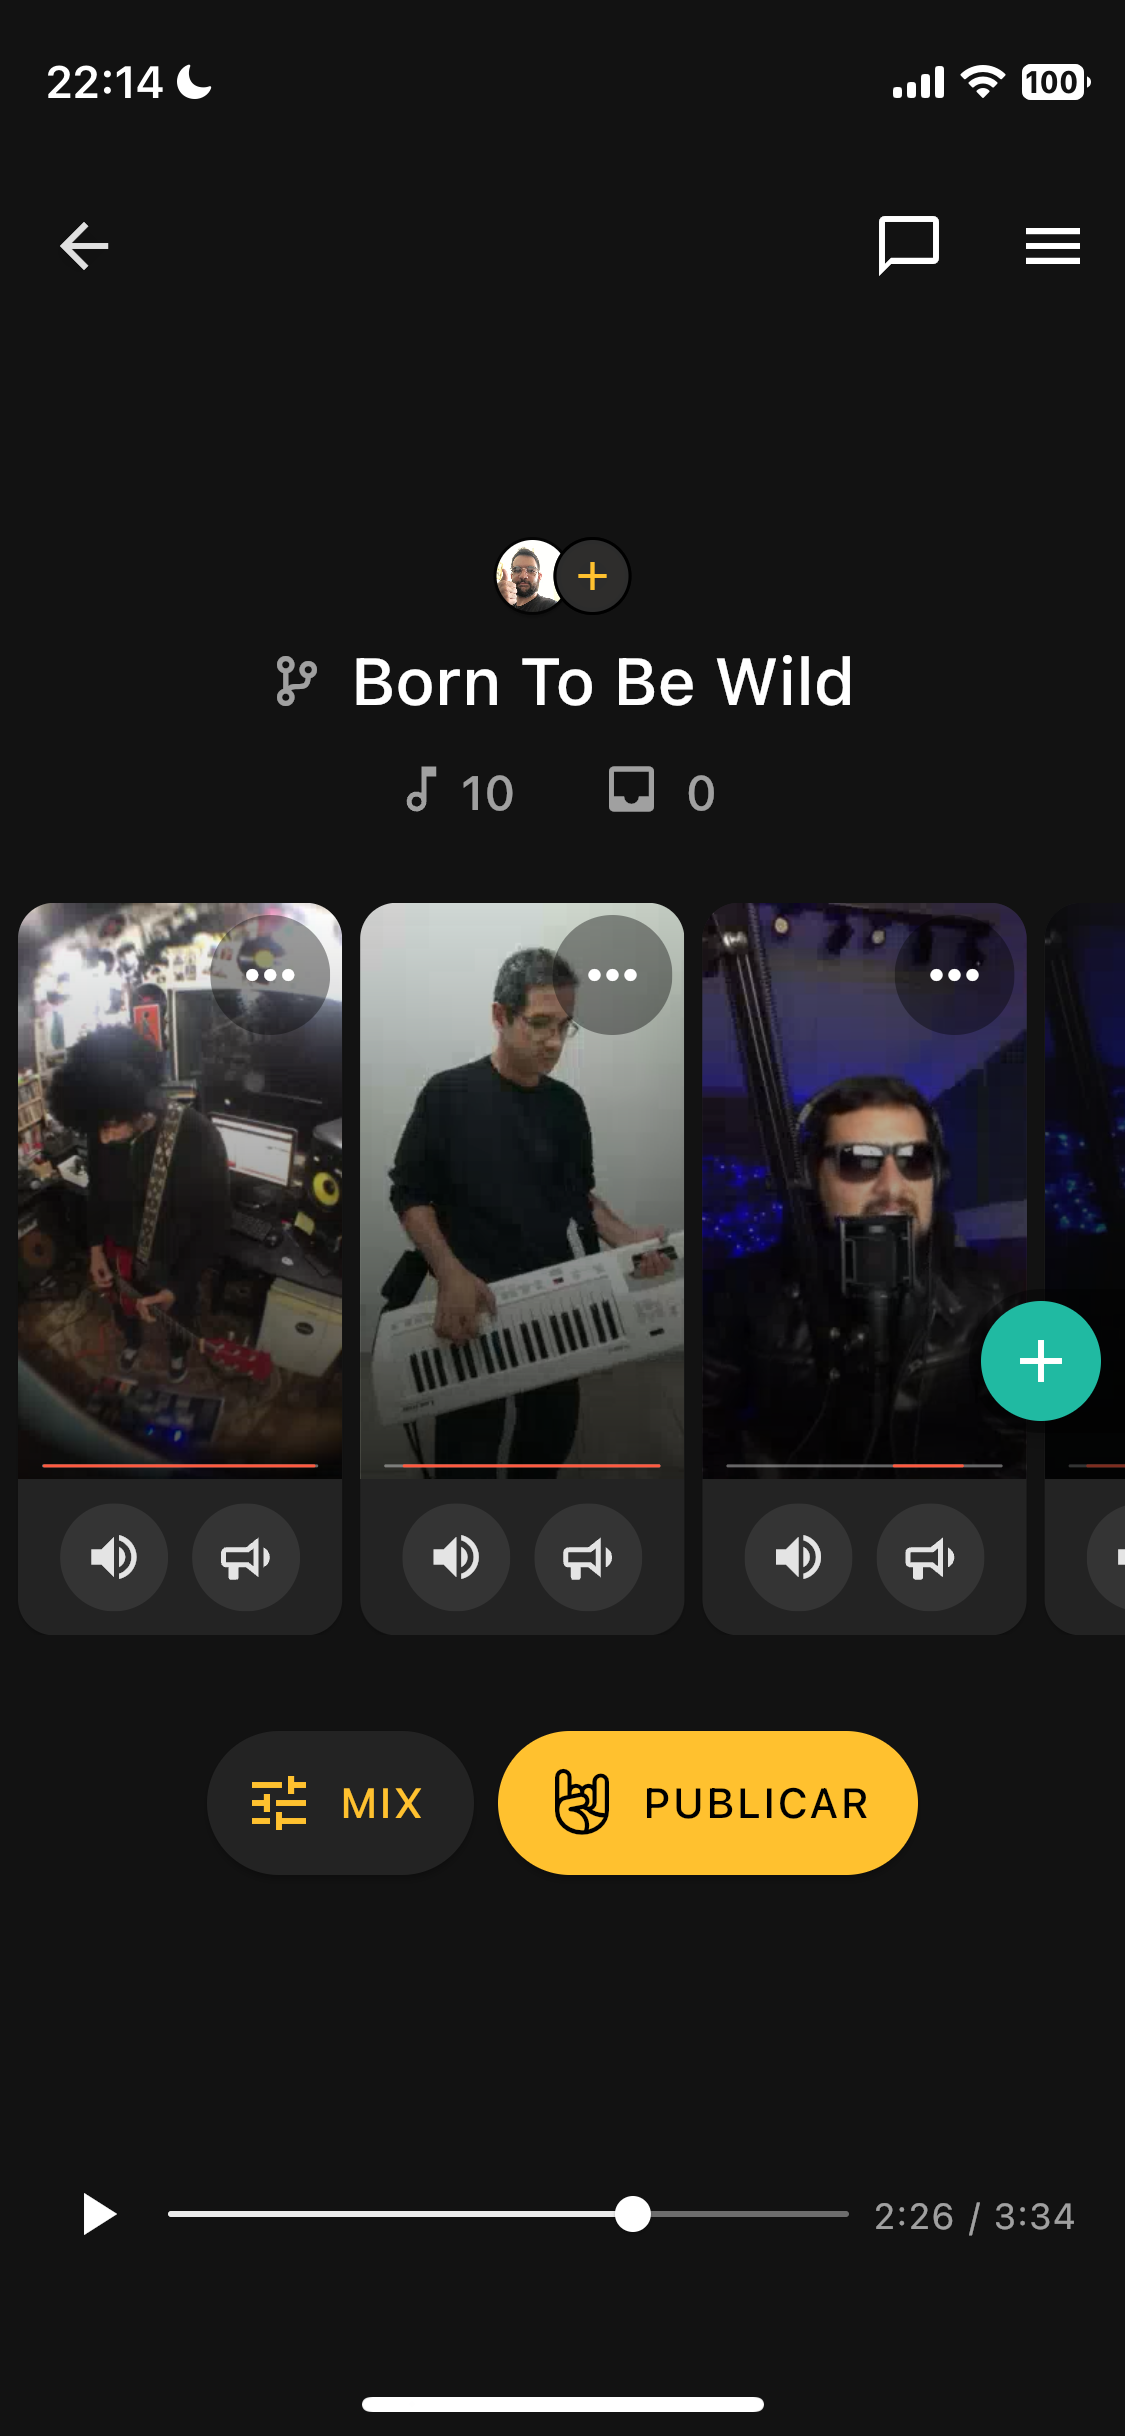
\includegraphics[width=0.24\textwidth]{chapters/chap01/images/inda/inda4.PNG}}
    \caption{Recursos do \textit{app Indaband}: (a) \textit{Home} (b) \textit{Feed} (c)
    \textit{Feed} (d) \textit{Studio}.}
    \label{fig:cap_tela}
\end{figure}

Indaband é uma aplicação móvel para distribuição e gravação de música
colaborativa e remota \cite{indaband}. A versão inicial foi disponibilizada
publicamente em Agosto de 2022. O quadro de funcionários é majoritariamente
brasileiro, enquanto que o produto possui distribuição global. A FIGURA
\ref{fig:cap_tela} exibe capturas de tela da interface visual.


O aplicativo móvel Indaband contém uma série de funcionalidades e abstrações
para a gravação e distribuição de música colaborativa. Para maior entendimento
do do sistema de recomendação a ser proposto, é necessário compreender as
principais entidades do aplicativo.


\subsubsection{Sessão}

Na aplicação, usuários podem criar sessões, que são ambientes colaborativos de
gravação entre os participantes. As sessões contam com ferramentas para gravação
e mixagem. O ambiente de pré-visualização, edição e produção da sessão chama-se
\textit{Studio}. Nesse ambiente, há funcionalidades de adição, edição,
remoção e mixagem de faixas. Sessão também é o nome dado ao conjunto de faixas
introduzidas pelos usuários que constituem uma determinada música.

A sessão contém uma funcionalidade de cabine de gravação, permitindo que os
participantes gravem faixas de áudio ou de vídeo. Além disso, o usuário pode
importar mídias de áudio ou de vídeo, tal que cada mídia importada equivale a
uma faixa.

O usuário que cria a sessão é considerado seu dono, enquanto os demais usuários
que aceitam o convite para ingressar são considerados participantes. Toda sessão
publicada é disponível para visualização pública e contém ao menos uma faixa. A
publicação pode ser posteriormente removida pelo dono da sessão.


\begin{figure}[h]
  \begin{center}
    \subfigure[]{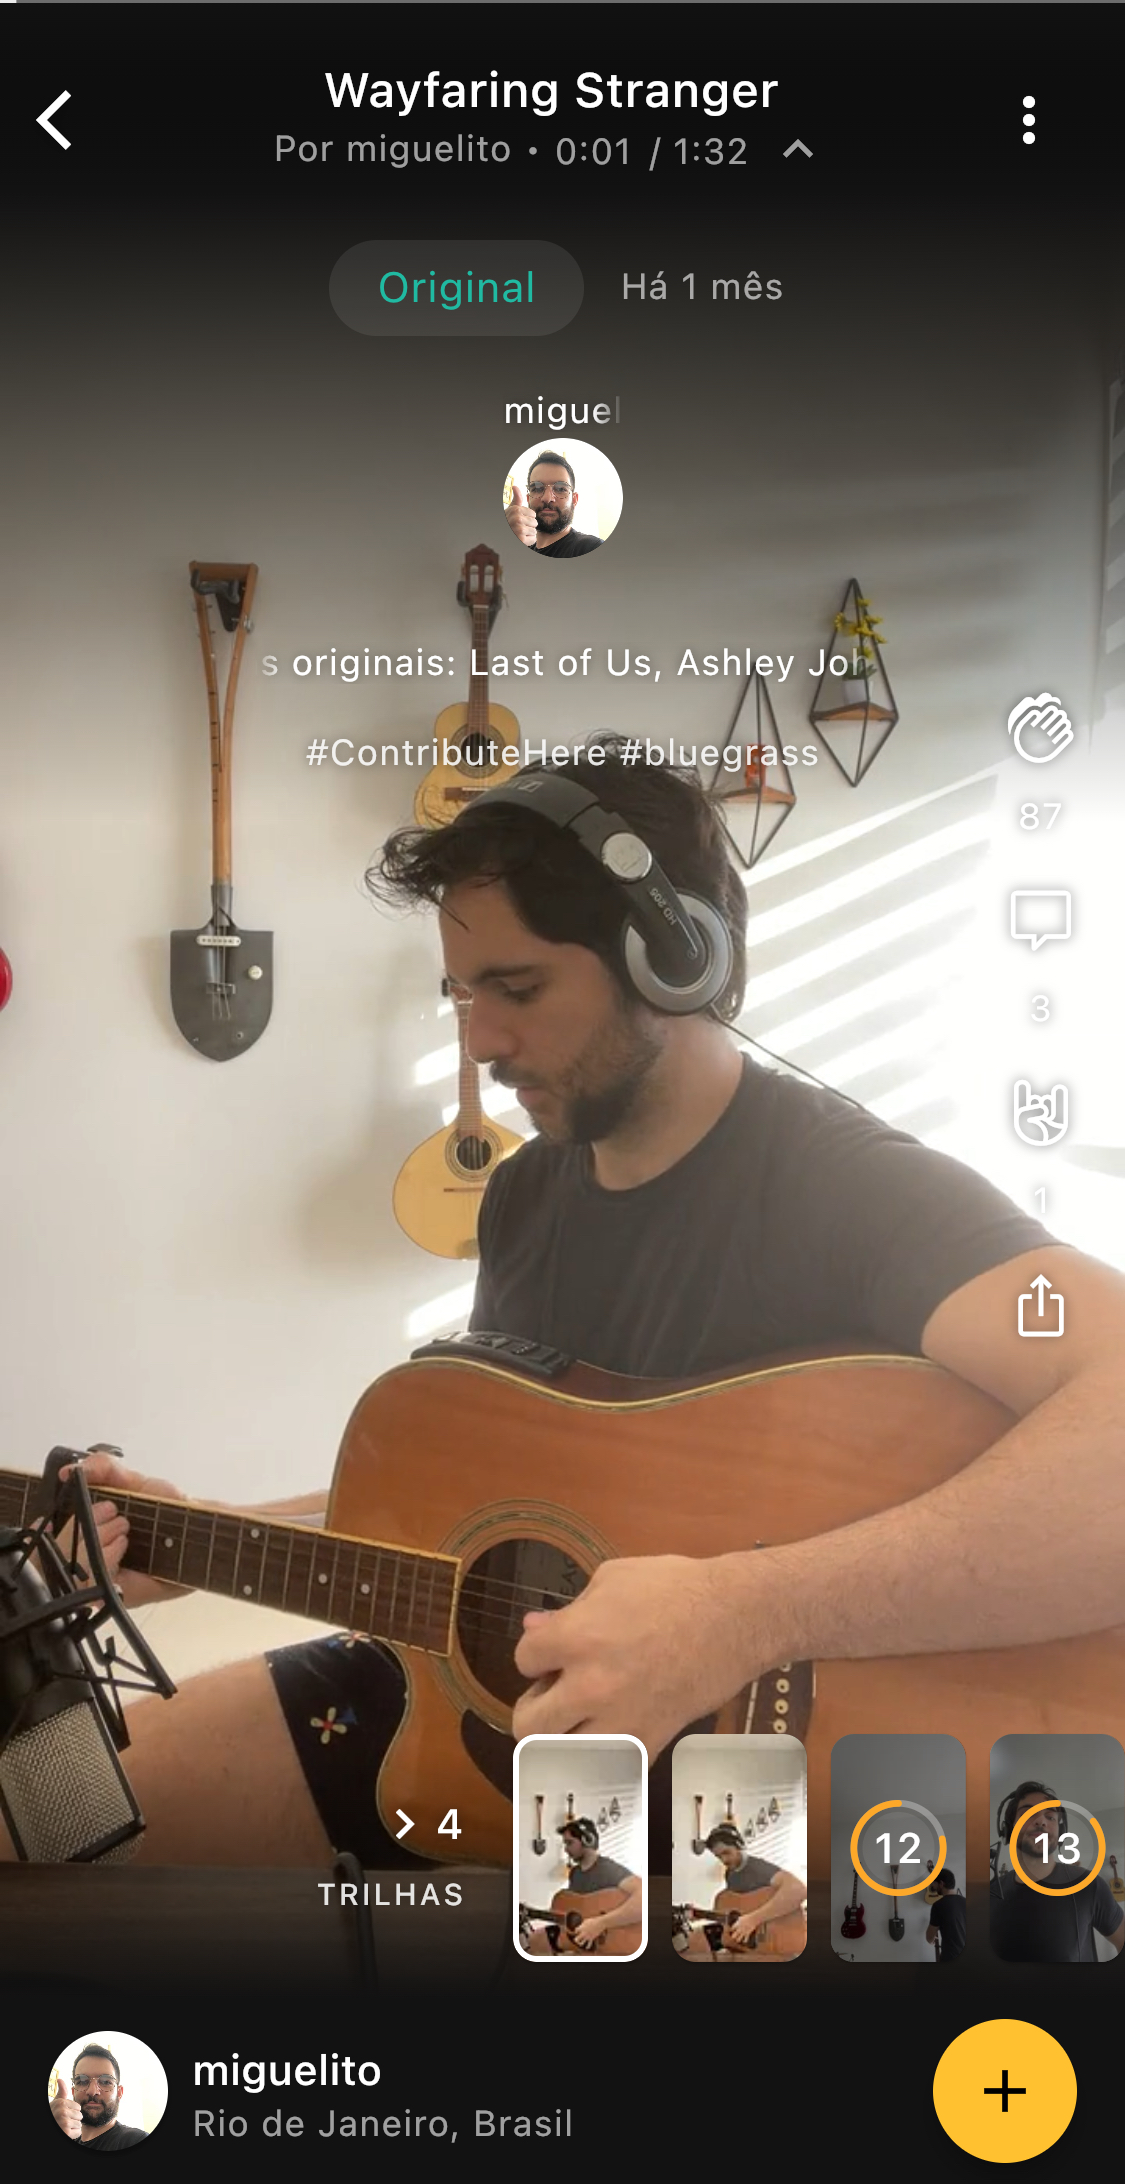
\includegraphics[width=0.4\textwidth]{chapters/chap02/images/wayfaring_original.jpeg}}
    \subfigure[]{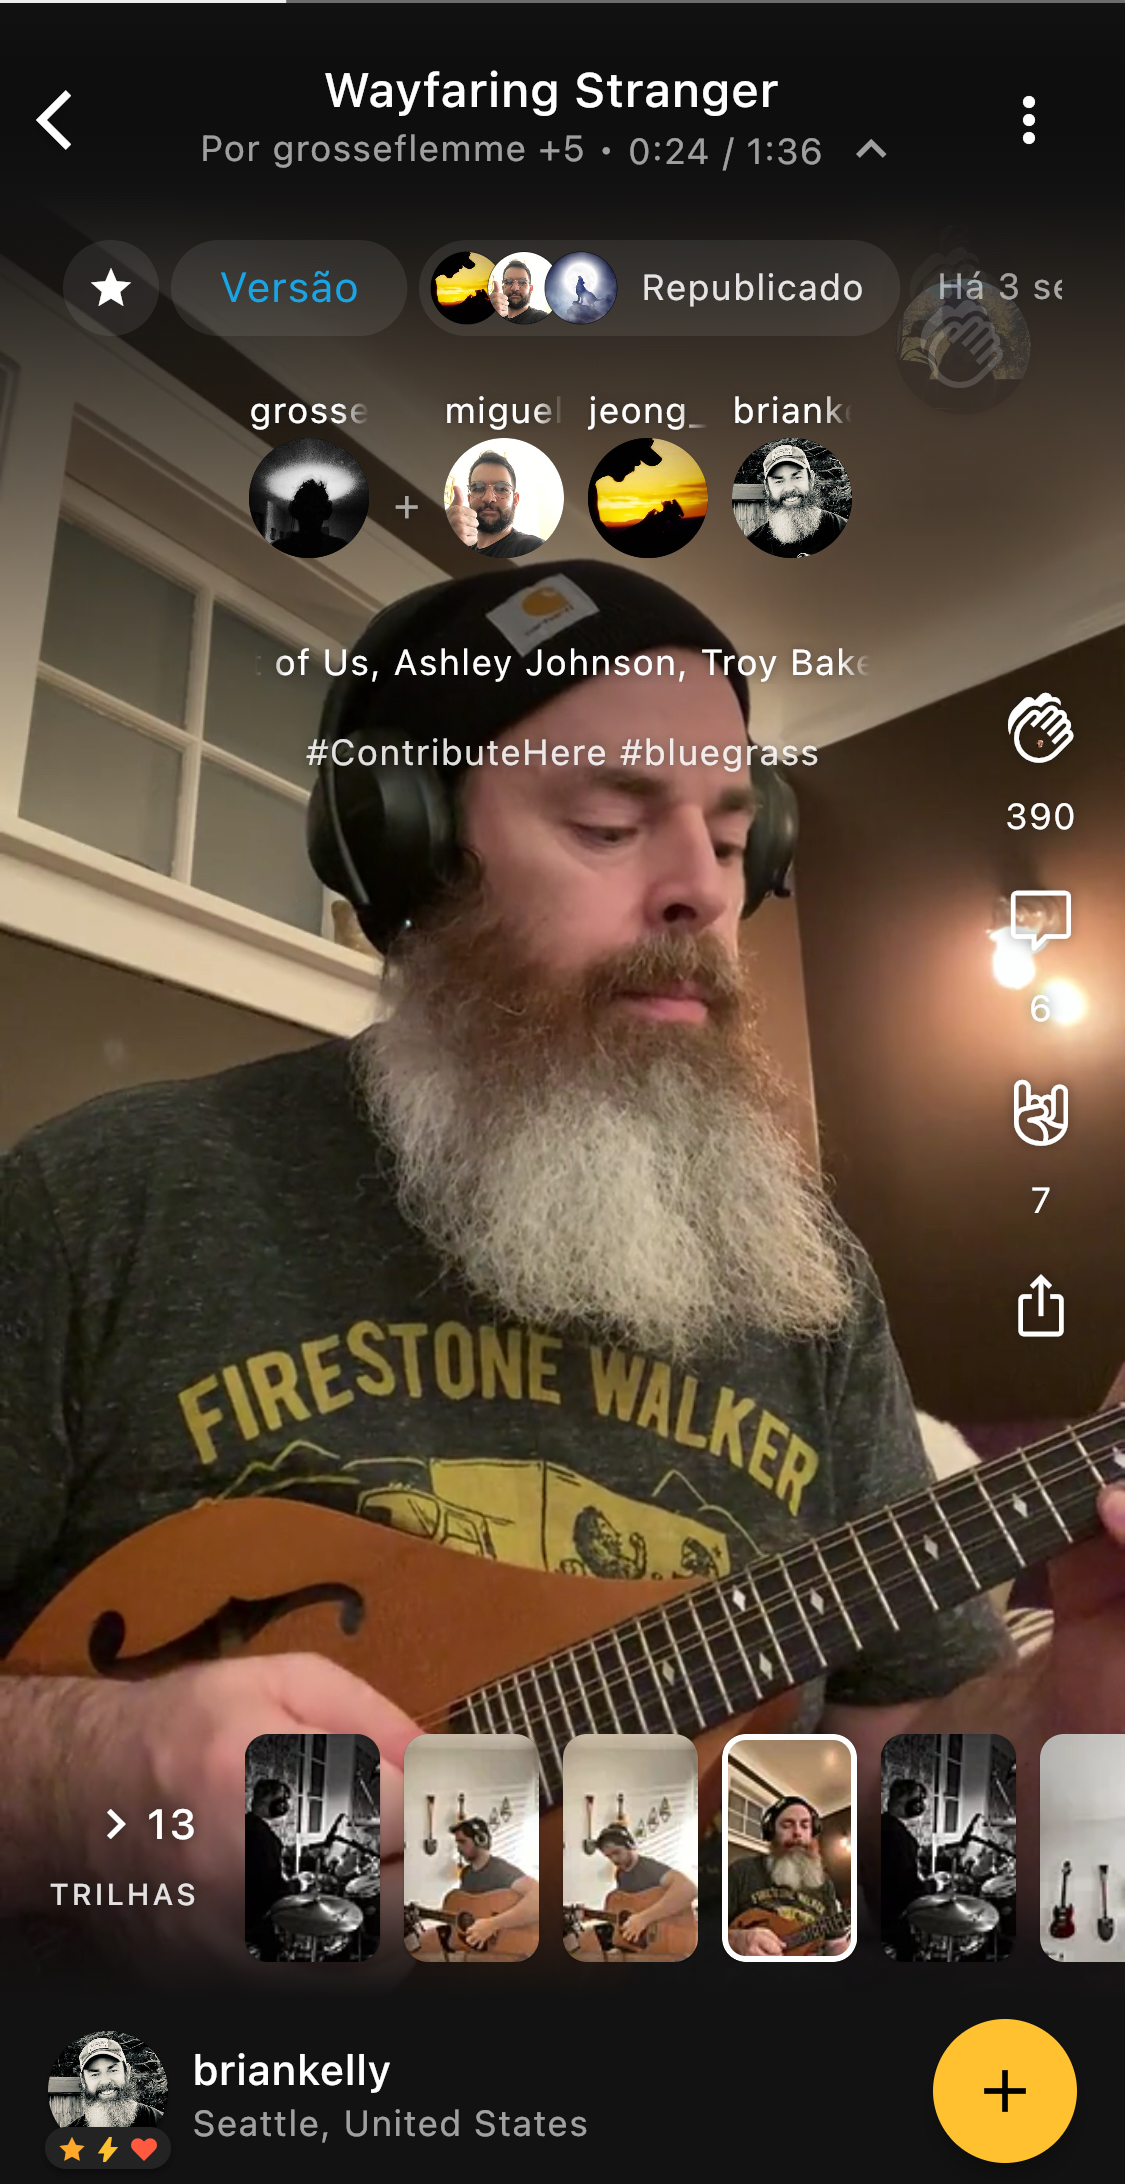
\includegraphics[width=0.4\textwidth]{chapters/chap02/images/wayfaring_fork.jpg}}
    \caption{Duas sessões publicadas no aplicativo Indaband. A primeira sessão é
    a sessão original, enquanto a segunda é um \textit{fork} subsequente da
    primeira. Ambas compartilham o mesmo nome e as faixas da primeira sessão. A
    segunda sessão contém faixas adicionais.}
    \label{fig:session_and_fork}
  \end{center}
  \end{figure}

\subsubsection{\textit{Fork}} Toda sessão publicada disponibiliza a
funcionalidade de \textit{fork} para os demais usuários da plataforma. O
\textit{fork} é uma cópia da sessão original, em que é possível adicionar
gravações inéditas, editar e remover faixas pré-existentes sem afetar a
publicação original. Quando publicada, a sessão \textit{fork} exibe o autor original das faixas
pré-existentes que forem mantidas, além da referência para a sessão anterior.

O \textit{fork} é uma das principais formas de colaboração assíncrona entre
usuários. A FIGURA \ref{fig:session_and_fork} ilustra duas sessões, sendo a
segunda um \textit{fork} subseqeuente da primeira. Note que a quantidade de
faixas e usuários presentes na segunda sessão aumenta. Além disso, conta com
maior quantidade de visualizações, comentários e outras formas de engajamento
positivo. Entre essas duas sessões, houve uma série de \textit{forks}
intermediários, realizados por cada um dos usuários que adicionaram faixas às
suas sessões.


\subsubsection{Faixa}
A faixa é uma mídia com áudio e vídeo que geralmente contém a gravação de um
instrumento ou voz. Uma faixa necessariamente é criada a partir de um entre três
recursos: tal como uma gravação original, tal como um \textit{fork} de uma faixa
publicada anteriormente ou como uma importação de uma mídia de áudio ou de
vídeo.




\section{Sobrecarga de informação}

Após três anos de desenvolvimento, a aplicação conta com dezenas de milhares de
usuários cadastrados, os quais centenas gravam mensalmente. Dado o grande
catálogo de usuários, o processo de encontrar pessoas com interesses musicais
similares demanda tempo e esforço. O mesmo ocorre ao procurar uma sessão que
seja de interesse em meio ao grande volume de conteúdo publicado. Essa
dificuldade percebida pelo usuário é conhecida na literatura de sistemas de
recomendação como sobrecarga de informação \cite{roetzel2019information}.

A sobrecarga de informação, segundo \citet{roetzel2019information}, é um estado em que um tomador de decisões observa um
conjunto ou uma carga de informações de complexidades distintas, a qual inibe a
capacidade do tomador de decisões de determinar de forma ótima a melhor decisão
possível.

\vspace{0.2cm}
\begin{figure}[h]
    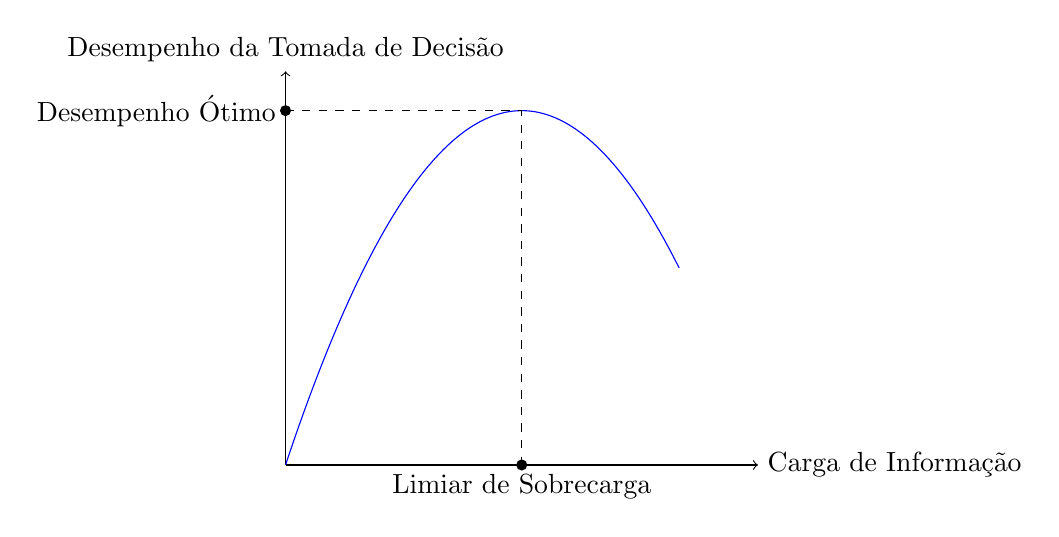
\begin{tikzpicture}
    % Eixo X
    \draw[->] (0,0) -- (6,0) node[right] {Carga de Informação};
    % Eixo Y
    \draw[->] (0,0) -- (0,5) node[above] {Desempenho da Tomada de Decisão};
  
    % Curva U invertida
    \draw[blue, domain=0:5, samples=100] plot (\x, {3*\x - 0.5*\x*\x});
  
    % Pontos de interesse
    \fill (0,4.5) circle (2pt) node[left] {Desempenho Ótimo};
    \fill (3,0) circle (2pt) node[below] {Limiar de Sobrecarga};

    % Linhas tracejadas
    \draw[dashed] (0,4.5) -- (3,4.5);
    \draw[dashed] (3,0) -- (3,4.5);
  \end{tikzpicture}
   % Descrição
    \caption{Correspondência entre a carga de informação e o desempenho da tomada
    de decisão.}
    \label{fig:u_invertida}
\end{figure}
\vspace{0.2cm}

O uso subótimo de informações é causado
pela limitação de recursos individuais escassos. Um recurso escasso pode ser uma
característica individual (como capacidade de processamento em série, memória de
curto prazo) ou equipamento relacionado à tarefa (por exemplo, orçamento ou
tempo para tomar uma decisão). A probabilidade de alcançar a melhor decisão
possível é definida como o desempenho de tomada de decisão. A correspondência
entre a carga de informação e o desempenho da tomada de decisão é ilustrada na
FIGURA \ref{fig:u_invertida} \cite{roetzel2019information}.

Experimentos realizados por \citet{liang2006personalized} mostraram que, ao
avaliar a satisfação de voluntários com um sistema de recomendação de notícias,
a precisão do conteúdo recomendado e o número de itens
recomendados influenciam diretamente na satisfação do usuário, reduzindo a
sobrecarga de informação e a insatisfação gerada pela sobrecarga.

\section{Sistemas de Recomendação}

\abbrev{RS}{sistemas de recomendação}
Sistemas de recomendação (RS, do inglês \textit{recommender systems}) são
ferramentas de \textit{software} que sugerem itens úteis para um usuário, de
acordo com a disponibilidade de seu histórico \cite{ricci2010introduction}. Esses
sistemas, que podem ser personalizados ou não-personalizados, ajudam usuários a
lidarem com processos de tomada de decisão em meio a sobrecarga de informações,
seja na escolha de um produto em um \textit{e-commerce} ou na seleção de um
filme em um serviço de \textit{streaming}. Ao contrário de uma ferramenta de
busca em que o usuário ativamente procura por um item específico, sistemas de
recomendação são úteis quando o usuário explora um catálogo diversificado,
otimizando a distribuição dos itens a partir de suas preferências pessoais. As
FIGURAS \ref{fig:spotify} e \ref{fig:twitter} ilustram sistemas de recomendação
para tarefas distintas: recomendação de \textit{playlists} na plataforma Spotify
e recomendação de perfis de usuário na plataforma Twitter, respectivamente.


\begin{figure}[ht]
    \centering
    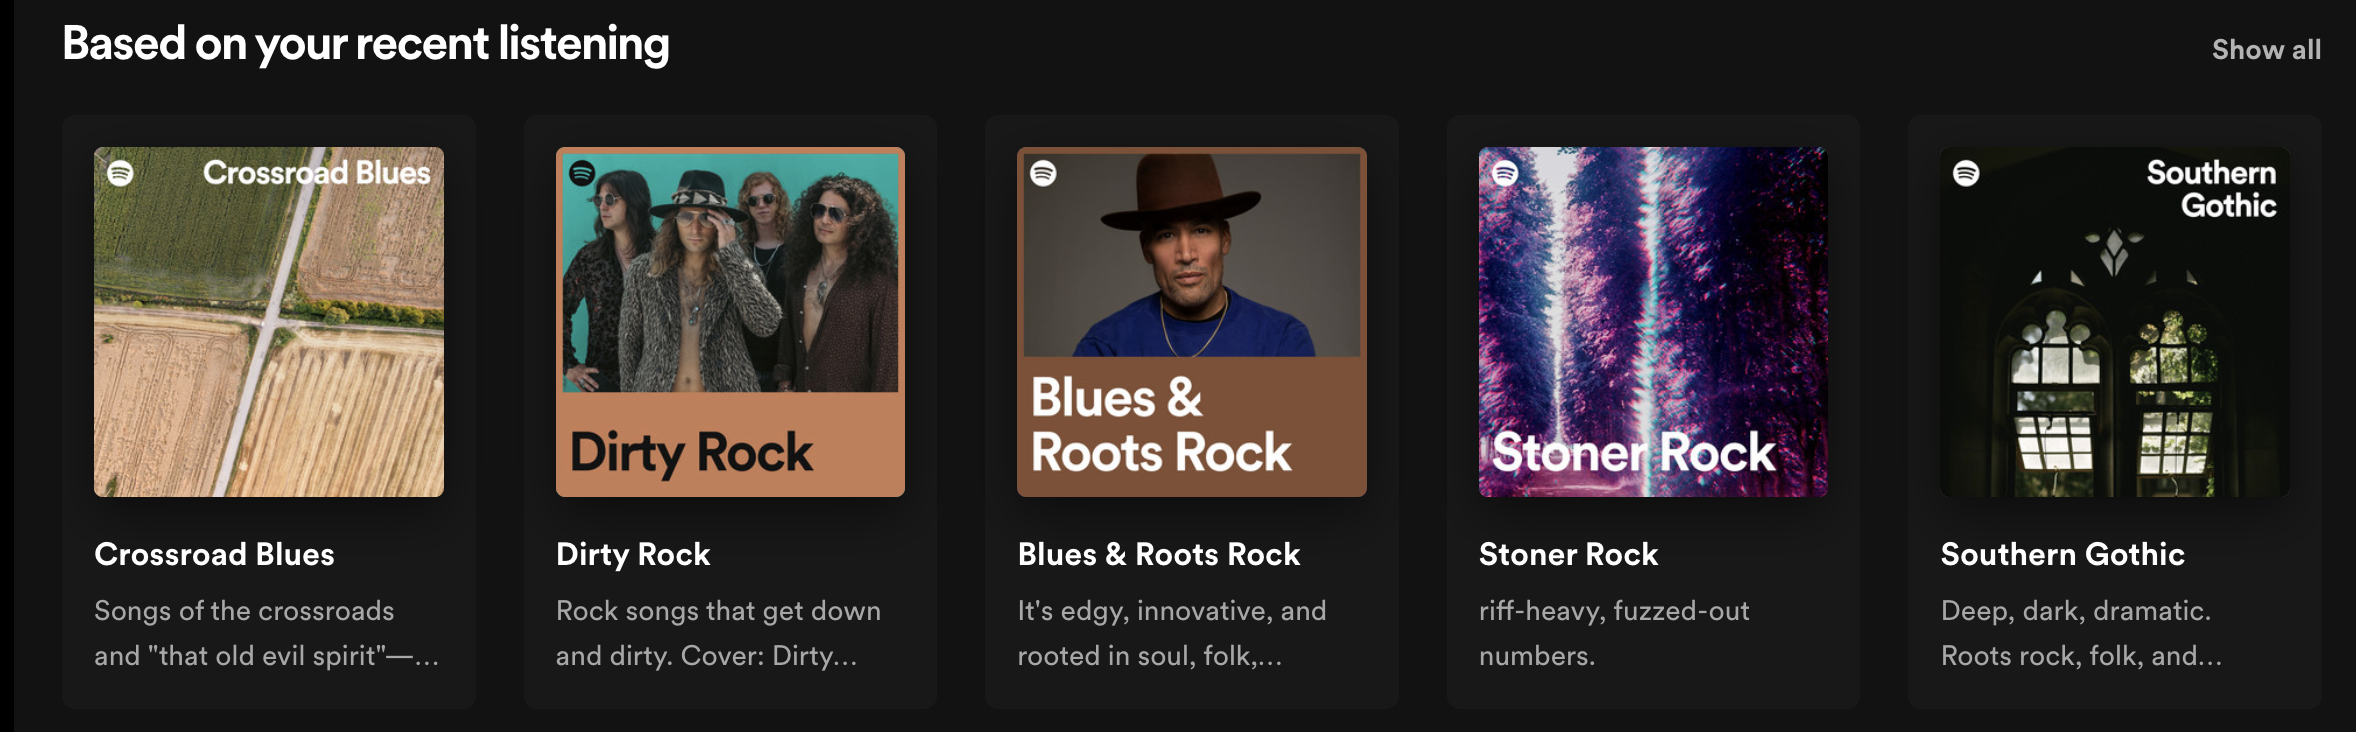
\includegraphics[width=0.8\textwidth]{chapters/chap01/images/spotify.png}
    \caption{Recomendações de \textit{playlists} no Spotify em Agosto de 2023.}
    \label{fig:spotify}
\end{figure}


Personalização é o processo de coleta e uso de informações pessoais para filtrar
conteúdo de forma única a um usuário, atendendo suas necessidades percebidas
pelo serviço ou declaradas explicitamente. \cite{liang2006personalized}.
Recomendações não-personalizadas distribuem o conteúdo recomendado de maneira
igualitária para todos os usuários, desconsiderando suas preferências
individuais. Uma recomendação a partir da lista de reportagens mais lidas em um
portal de notícias é um exemplo de recomendação não-personalizada.
\cite{falk2019practical}.

\begin{figure}[ht]
    \centering
    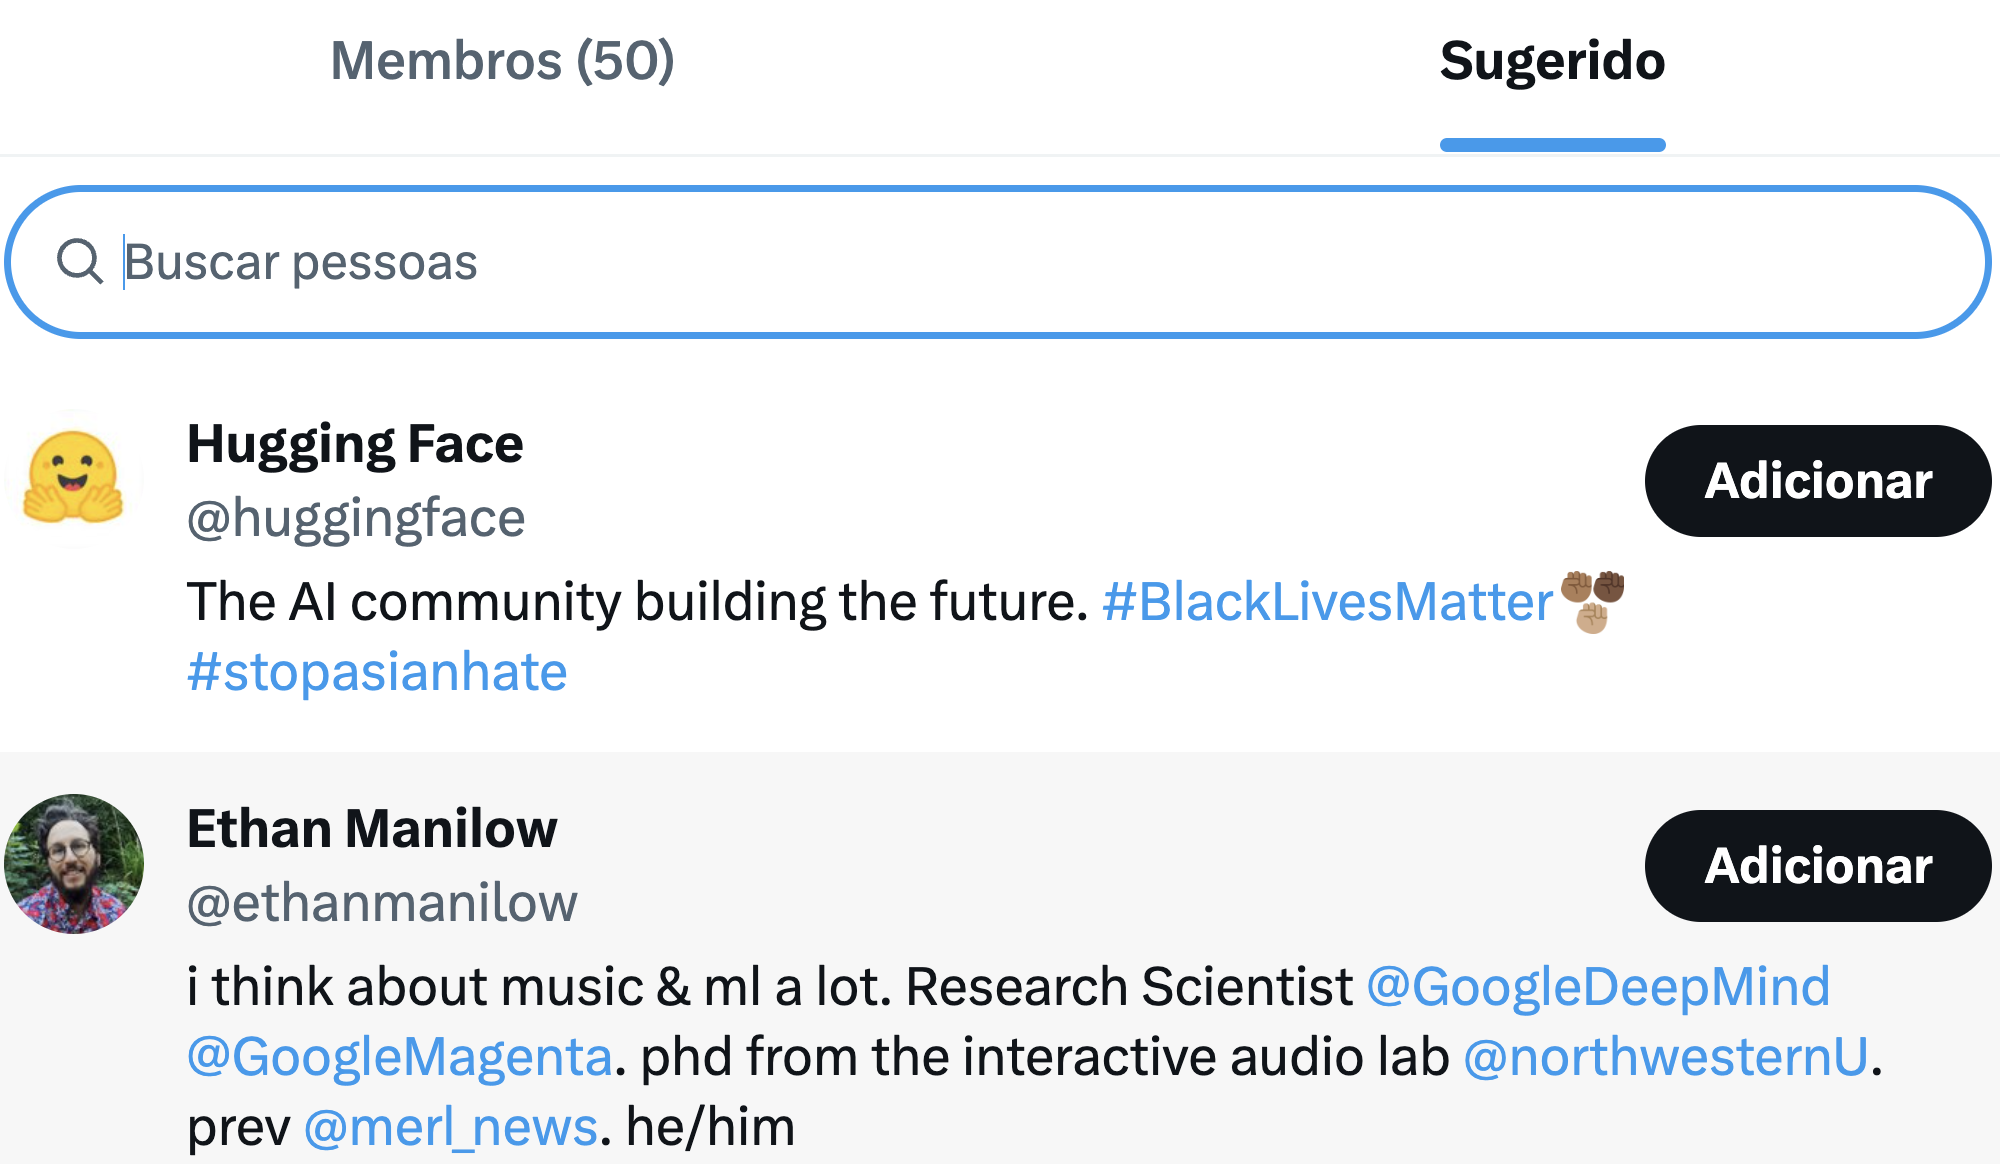
\includegraphics[width=0.6\textwidth]{chapters/chap01/images/tt.png}
    \caption{Recomendações de perfis de usuário no Twitter em Agosto de 2023.}
    \label{fig:twitter}
\end{figure}

% Sistemas de Recomendação Baseados em Sessão (SBRS, do inglês
% \textit{session-based recommender systems}) são sistemas de recomendação que 
Abordagens mais tradicionais em sistemas de recomendação modelam as interações
usuário-item na forma de uma matriz esparsa de avaliações. Cada linha da matriz
representa um usuário e cada coluna representa um item.

A tarefa em questão se
resume ao preenchimento dos valores faltantes da matriz, a depender da
abordagem escolhida. Valores preenchidos com avaliações altas são recomendados
ao usuário, uma vez que ele ainda não os consumiu, tal como ilustrado
na FIGURA \ref{fig:matriz_15}.


\begin{figure}[h]
    \centering
    \begin{tikzpicture}
        % Define the matrix
        \matrix (m) [matrix of nodes,
                    %  nodes in empty cells,
                     column sep=-\pgflinewidth,  % Adjust cell spacing
                     row sep=-\pgflinewidth,     % Adjust cell spacing
                     nodes={draw, text width=2.5em, align=center, minimum height=2.5em, minimum width=2.5em}] {
            5 & 4 & 1 & 1 \\
            4 & 4 & 1 & 1 \\
            1 & 2 &  & 4 \\
            1 & 1 & 4 & 4 \\
        };
      
        % % Labels on the left
        \foreach \row/\label in {1/Gilberto, 2/Maria, 3/Gal, 4/Caetano} {
          \node[left] at (m-\row-1.west) {\label};
        }
      
        % % Labels on the top
        \foreach \col/\label in {1/TV, 2/DVD, 3/sal, 4/pipoca} {
          \node[above,
          ] at (m-1-\col.north) {\label};
        }
      \end{tikzpicture}
      \caption{Matriz de avaliações para produtos de um comércio eletrônico. A predição atua sobre as avaliações não preenchidas.}
      \label{fig:matriz_15}
\end{figure}

\abbrev{SBRS}{Sistemas de recomendação baseados em sessão}
Por mais que a matriz de avaliações seja uma forma intuitiva de representação,
viabilizando uma boa variedade de modelos, trata-se de uma forma que
desconsidera o contexto temporal das interações ou a sequência específica de
itens que determinado usuário interagiu. Sistemas de Recomendação Baseados em
Sessão (SBRS, do inglês \textit{session-based recommender systems}) atuam
justamente nesse cenário.

Os SBRS se caracterizam pelos seus dados representarem um conjunto delimitado de
interações obtidas por \textit{feedback} implícito, ou seja, por preferências
indiretas identificadas a partir de ações ou padrões de navegação. Essas interações
são agrupadas em conjuntos denominados sessões. Uma sessão pode conter uma sequência temporalmente
ordenada de ações executadas por um usuário, ou um conjunto de ações executadas
por um usuário anônimo sem uma ordem específica.

Os objetivos de um SBRS incluem
prever a próxima interação do usuário durante uma sessão em andamento,
recomendar o próximo item ou um conjunto de itens para uma sessão, ou ainda
recomendar uma sessão inteira \cite{domingues_large_2023, survey_wang_2021}.


    



\begin{figure}[h]
    \centering
        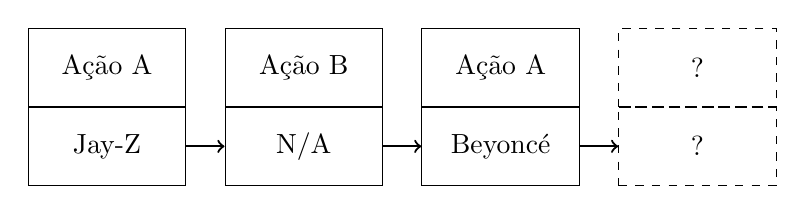
\begin{tikzpicture}
        % Draw the list cells
        \node[draw, rectangle, minimum width=2cm, minimum height=1cm] (cell1) at (0, 0) {Jay-Z};
        \node[draw, rectangle, minimum width=2cm, minimum height=1cm] (cell2) at (2.5, 0) {N/A};
        \node[draw, rectangle, minimum width=2cm, minimum height=1cm] (cell3) at (5, 0) {Beyoncé};
        \node[draw, dashed, rectangle, minimum width=2cm, minimum height=1cm] (cell4) at (7.5, 0) {?};

        % Draw the arrow
        \draw[->, thick] (cell1.east) -- (cell2.west);
        \draw[->, thick] (cell2.east) -- (cell3.west);
        \draw[->, thick] (cell3.east) -- (cell4.west);

        % % Add label to the left of the first cell
        % \node[left] at (cell1.west) {Sessão 1};

        % Draw the top cells with actions
        \node[draw, rectangle, minimum width=2cm, minimum height=1cm] (topcell1) at (0, 1.0) {Ação A};
        \node[draw, rectangle, minimum width=2cm, minimum height=1cm] (topcell2) at (2.5, 1.0) {Ação B};
        \node[draw, rectangle, minimum width=2cm, minimum height=1cm] (topcell3) at (5, 1.0) {Ação A};
        \node[draw, dashed, rectangle, minimum width=2cm, minimum height=1cm] (topcell4) at (7.5, 1.0) {?};

    \end{tikzpicture}
    \caption{Exemplo de uma sessão em andamento.}
    \label{fig:sessao_beyonce}
\end{figure}

Cada interação das sessões está associada a tuplas que contém um ou mais dos
seguintes dados: a ação executada, o item alvo da ação, o instante em que a ação
foi executada e o usuário responsável pela ação. Por exemplo, uma sessão pode
representar uma lista ordenada de itens selecionados por um usuário anônimo, ou
uma lista de ações executadas por usuários de uma mesma sessão, sem que essas
ações estejam necessariamente atreladas cada uma a um item. Isso é um aspecto
útil dos SBRS, por prover recomendações em aplicações em que não há distinção
entre usuários, ou quando as preferências de longo prazo de um usuário novo da
plataforma não foram identificadas. A FIGURA \ref{fig:sessao_beyonce} ilustra um
exemplo de sessão em andamento, em que a ação A corresponde a navegar ao perfil
de determinado artista, enquanto que a ação B corresponde a criar uma
\textit{playlist} vazia. Nem toda ação é necessariamente associada a um item,
como expresso na Ação B.
\vspace{0.4cm}
\section{Trabalhos Futuros}
% TODO: @Miguel - Needs review

A bibliografia existente de espectrograma de modulação, até o presente momento,
aplica uma segunda STFT sobre o domínio acústico, com a finalidade de medir
oscilações de intensidade no eixo da frequência. Dessa forma, o novo eixo obtido
pelo espectrograma de modulação representa modulações de amplitude.

Considerando
que o espectrograma acústico reside em um espaço vetorial $\mathbb{R}_3$, uma proposta de trabalho futuro é
investigar a possibilidade de representar modulações em frequência, bastando que a segunda
STFT meça as oscilações no eixo da frequência para uma dada intensidade
constante.
  %%________________________

  \backmatter
  
  \bibliographystyle{configs/coppe-unsrt}
  \bibliography{main}

  \appendix
  % \chapter{Algumas Demonstra{\c c}\~oes}
\end{document}
